\chapter{\mbox{Implicit generative models}}\label{ch:differentiable-generative-models}

%The approximate inference methods considered so far in Chapters \ref{ch:approximate-inference} and \ref{ch:pseudo-marginal-methods} have been aimed at dealing with various forms of computational intractability in probabilistic models. In Chapter \ref{ch:probabilistic-modelling}-modelling} we motivated that the key computational challenges in inference problems is generally the computation of integrals which do not have an analytic solution and which are intractable to compute using standard quadrature numerical integration methods. In Chapter \ref{ch:approximate-inference} we considered various methods which have been proposed for computing approximations to these intractable intractables, in particular focussing on \ac{MCMC} methods as a very generally applicable family of methods which are able to give asymptotically exact estimates in the limit of infinite computation.
%
%The sampling and optimisation
%
%In the preceding chapter we considered the pseudo-marginal framework, which allows \ac{MCMC} methods to be applied given only an unbiased estimator for the density function of the target distribution. This allows 
%
%
%
%In the preceding chapter we considered the pseudo-marginal framework, which allows \ac{MCMC} methods to be extended from the standard approximate inference case in which we can evaluate a generally unnormalised density function for the target distribution of interest, to problems in which we may only have access to a unbiased (and non-negative) estimator for this function. A key idea exploited in the previous chapter 
%
% applied to problems in which we only have access to an unbiased and non-negative estimator for a density function of the target distribution of interest.
%
%
%In this chapter we will consider approximate inference methods for dealing with another form of intractability: probabilistic models specified by a generative process in which the density of the model variables is defined only \emph{implicitly} \citep{beaumont2002approximate,gourieroux1993indirect,diggle1984monte}. In such \emph{implicit generative models} we can generate sample values for the variables in the model, but we cannot tractably evaluate the probability distribution of those variables or more specifically its density with respect to an appropriate base measure. 
%
%
% A further level of intractability arises for probabilistic models specified by a generative process in which the density of the model variables is defined only \emph{implicitly} \citep{beaumont2002approximate,gourieroux1993indirect,diggle1984monte} - that is we can generate sample values for the variables in the model, but we cannot tractably evaluate the probability distribution of those variables or more specifically its density with respect to an appropriate base measure. 
%
%
%Probabilistic models can exhibit various forms of computational intractability.
%
%In many inference problems th
%
%
%Probability density functions have played a central role in the approximate inference methods considered so far in this thesis. The approximate inference methods considered in Chapter \ref{ch:approximate-inference} required that we are able to evaluate an explicit probability density function for the target distribution of interest. In many inference problems the target density function is only evaluable up to to an unknown intractable normalising constant. Both the sampling and optimisation based inference approaches considered however are generally able to cope with this ambiguity. In the preceding chapter we considered the pseudo-marginal framework, which allows \ac{MCMC} methods to be applied given only an unbiased non-negative estimator of the target density of interest. One context in which pseudo-marginal methods are applied is in so-called `doubly-intractable' distributions \citep{murray2006mcmc} where the target distribution of interest involves
%
%The approximate inference methods considered so far in this thesis have been focussed on probabilistic models specified via an explicit joint probability density function on the model variables. Both the sampling and optimisation based inference approaches reviewed in Chapter \ref{ch:approximate-inference} required evaluation 
%
% A further level of intractability arises for probabilistic models specified by a generative process in which the density of the model variables is defined only \emph{implicitly} \citep{beaumont2002approximate,gourieroux1993indirect,diggle1984monte} - that is we can generate sample values for the variables in the model, but we cannot tractably evaluate the probability distribution of those variables or more specifically its density with respect to an appropriate base measure. 

%In many inference problems $\tgtdens$ is only evaluable up to to an unknown normalising constant $Z$ however both sampling and optimisation based inference approaches are generally able to cope with this ambiguity, and in some cases such as importance sampling are able to estimate $Z$ itself. 

In the approximate inference methods considered in Chapter \ref{ch:approximate-inference} a unifying element was the requirement to be able to evaluate an explicit probability density function for the target distribution of interest. In the previous chapter we considered the pseudo-marginal framework which allowed relaxing this requirement to being able to evaluate an unbiased (and non-negative) estimator for the target density. In this chapter we will consider probabilistic models specified by a generative process in which the density of the model variables is defined only \emph{implicitly} \citep{beaumont2002approximate,gourieroux1993indirect,diggle1984monte} - that is we can generate sample values for the variables in the model, but we cannot tractably evaluate the probability distribution of those variables or more specifically its density with respect to an appropriate base measure. 

Although models without an explicit density function are challenging to work with from an inferential perspective, they are ubiquitous in science and engineering in the form of probabilistic models defined by the computational simulation of a physical system. Typically simulator models are specified procedurally in code with any stochasticity introduced by drawing values from a pseudo-random number generator. %We previously briefly discussed an example of a simulator model based on the approximate integration of a set of \acp{SDE} when considering graphical models in Section \ref{subsec:simulators} of Chapter \ref{ch:probabilistic-modelling}. 
The complexity of the function mapping from random inputs to simulated outputs typically makes calculating an explicity density on the outputs at best non-trivial and often intractable (as seen for a simple example in Figure \ref{fig:example-non-bijective-transform-factor-graph} in Chapter \ref{ch:probabilistic-modelling}).
%. In the common case where the simulator outputs cannot be expressed as an injective function of (potentially a subset of) the random inputs the density on the model variables will usually not have a closed form expression.
%Often the function mapping from random inputs to outputs in a simulator model will be non-injective. This means that analytically computing a probability density on the simulator outputs is usually intractable as it involves the generalised change of variables formula \eqref{eq:change-of-variables-vector} introduced in in Chapter \ref{ch:probabilistic-modelling} \S \ref{subsec:change-of-variables} which requires finding the pre-image of an output point in the input space and integrating across this set, which will typically be a complex implicitly defined non-linear manifold.

There has also been a long history in statistics of using distributions defined by their quantile function \citep{hastings1947low,tukey1960practical} from which we can easily generate independent samples using the inverse transform sampling method discussed in Chapter \ref{ch:approximate-inference}. Although these \emph{quantile distributions} are often able to offer very flexible descriptions of shape of a distribution \citep{gilchrist2000statistical} 
often the quantile functions will not have an analytic inverse meaning their \ac{CDF} and so density function cannot be evaluated analytically. Generative models in which the density of the model variables is only defined implicitly have also been the subject of substantial recent interest in the machine learning community due to the development of effective training approaches which do not require evaluation of a density on the model variables \citep{li2015generative,dziugaite2015training,goodfellow2014generative}, with there being significant gains in modelling flexibility by dropping the requirement to be able to compute an explicit density function \citep{mohamed2016learning,tran2017deep}.

%, with a second \emph{encoder} model used as an inference network which given an observed data point outputs the parameters of a variational approximation to the corresponding posterior density under the decoder model $\pden{\rvct{h}|\rvct{y}}$. The encoder and decoder network 

%The focus of this chapter will therefore be methods for using generative models where we do not necessarily have access to an explicit density on the model variables, to make inferences about unobserved variables given known values for a set of observed variables. 
The focus of this chapter will therefore be methods for performing approximate inference in generative models where we do not necessarily have access to an explicit density on the model variables. 
%For example given a generative model of images we may wish to infer plausible in-paintings of an image region given knowledge of the surrounding pixel values. Similarly given a simulator model of a physical process and generator of model parameters which we believe are reasonable a priori, we may wish to infer our posterior beliefs about the parameters given the model and observations of the process. 
A lack of an explicit density function makes it non-trivial to directly apply the approximate inference approaches that have been discussed so far in this thesis. This has spurred the development of inference approaches specifically targeted at implicit generative models such as indirect inference \citep{gourieroux1993indirect} and \acf{ABC} \citep{beaumont2002approximate}.%, with their use particularly prevalent in respectively econometrics and computational biology.
 %Both \ac{ABC} and indirect inference methods have been successfully applied to perform inference in a range of complex probabilistic models, with their use particularly prevalent in respectively population genetics and econometrics.
 
%This approximation that the simulated observations are only close but not equal to the observed data makes the inference problem more tractable, but also changes the effective model inference is being performed on and so.
 
In both indirect inference and \ac{ABC}, inferences about plausible values of the unobserved variables are made by computing distances between simulated observed variables and observed data. At a qualitative level, values of the unobserved variables associated with simulated observations that are `near' to the data are viewed to be more plausible. This approximation that the simulated observations are only close but not equal to the observed data makes the inference problem more tractable, but also biases the inference output. Further simple distance measures tend to become increasingly less informative as the dimensionality of a space increases, making it challenging to use these approaches to perform inference in models with large numbers of unobserved variables. This motivates the use of dimensionality reduction techniques to project the observations to a set of lower-dimensional summary statistics. Although through careful choice of summaries this approach can yield good results, identifying informative summaries is challenging and except for rare cases where sufficient statistics are available any reduction to summary statistics will entail a loss of information about the unobserved variables compared to conditioning on all observations.

We make two main contributions in this chapter. First we show that by reparameterising the approximate conditional expectations estimated in \ac{ABC} approaches to inference in generative models it is possible to express them in the form of an expectation of a function of a random vector variable distributed according to a density which we can evaluate up to a normalising constant. This makes it possible to apply efficient general purpose approximate inference methods such as slice sampling and Hamiltonian Monte Carlo to implicit generative models without the need to develop dedicated \ac{ABC} variants. It is sometimes feasible to apply these methods when conditioning on all observations without the need to reduce dimensionality using summary statistics. The reparameterisation used is closely related to that applied to pseudo-marginal density estimators in the previous chapter, with existing \ac{ABC} \ac{MCMC} methods being a common special case of the pseudo-marginal Metropolis--Hastings update discussed there.

Secondly for a restricted class of generative models we term differentiable generative models and which we define in a following section, we show that it is possible to express exact conditional expectations under the model as integrals against a density we can evaluate pointwise across an implicitly defined manifold. We use this to propose a novel constrained \ac{HMC} method for performing inference in differentiable generative models. Unlike \ac{ABC} approaches, this method allows inference to be performed by conditioning the observed variables in the model to be within arbitary small distances of the data values while remaining computationally tractable.

The contributions described in this chapter have previously appeared in the published conference paper
\begin{itemize}
 \item \resizebox{0.92\columnwidth}{!}{Asymptotically exact inference in differentiable generative models.}\\ Matthew M. Graham and Amos J. Storkey. \emph{Proceedings of the 20th International Conference on Artificial Intelligence and Statistics, \\PMLR 54:499-508}, 2017.
\end{itemize}
I was the primary author of that work and proposed the novel contributions made in the paper. I also performed and analysed the numerical experiments described in the paper, some of which are reproduced in this chapter in Section \ref{sec:dgm-experiments}. This chapter expands upon the analysis and discussion in the above publication and includes additional numerical experiments.


%across an implicitly defined manifold gainst a density we can evaluate pointwise with respect to the Hausdorff measure for an implicitly defined manifold

%We will describe a novel \ac{HMC} method for performing inference in important sub-class of implicitly-defined generative models where the mapping from random inputs to the model to simulated observed and latent variables is differentiable. Unlike existing approaches, this method allows inference to be performed by conditioning the observed variables in the model to be within arbitary small distances of the data values while remaining computationally tractable. Further by exploiting gradient information the approach is able to perform efficient inference in models with large numbers of unobserved variables and conditioning on all observed data rather than low-dimensional summaries as is common in \ac{ABC} approaches.


% This means that subject to the conditions of the Markov chain being irreducible and aperiodic as discussed in Chapter \ref{ch:approximate-inference} Section \ref{subsec:markov-chain-monte-carlo}, asymptotically exact inference can be performed: conditional expectation estimates computed using the method will converge in the asymptotic limit to their true values.

\section{Differentiable generator networks}

\begin{figure}[!t]
\centering
\begin{subfigure}[t]{.35\linewidth}
\centering
\includetikz{gan-generator}
\caption{\acs{GAN} generator}\label{sfig:gan-generator}
\end{subfigure}%
\begin{subfigure}[t]{.55\linewidth}
\centering
\includetikz{gaussian-vae-decoder}
\caption{Gaussian \acs{VAE} decoder}\label{sfig:vae-decoder-marginalised}
\end{subfigure}%
\\[3mm]
\begin{subfigure}[t]{.8\linewidth}
\centering
\includetikz{reparam-gaussian-vae-decoder}
\caption{Reparameterised Gaussian \acs{VAE} decoder}\label{sfig:vae-decoder}
\end{subfigure}%
\caption[Differentiable generator network factor graphs.]{Example factor graphs for the generator of a \ac{GAN} and decoder of a \ac{VAE}. \subref{sfig:gan-generator} The generator for a \ac{GAN} with a standard normal distribution on the hidden code $\rvct{h}$, this mapped through a differentiable network $\vctfunc{g}_{\vct{\theta}}$, to generate the simulated output vector $\rvct{y}$. \subref{sfig:vae-decoder-marginalised} The decoder of a Gaussian \ac{VAE}. Again a hidden code vector $\rvct{h}$ with a standard normal distribution is used, differentiable network functions $\vctfunc{m}_{\vct{\theta}}$ and $\vctfunc{s}_{\vct{\theta}}$ then mapping from this code vector to mean and diagonal covariance parameters of a multivariate normal distribution on the output vector $\rvct{y}$. \subref{sfig:vae-decoder} The same \ac{VAE} decoder model as \subref{sfig:vae-decoder-marginalised}, with in this case the conditional factor on the outputs $\rvct{y}$ given hidden code $\rvct{h}$ reparameterised in terms of a deterministic transformation of a standard normal vector $\rvct{n}$.}
\label{fig:gan-and-vae-factor-graphs}
\end{figure}

%This highlights the key property of differentiability and avoids conflation with biological neural networks.
We first review two approaches to specifying generative models using differentiable networks\footnote{A a differentiable parametric function formed by interleaving `layers' of affine transformations and elementwise non-linearities, also termed a \emph{neural network}.}, \acfp{GAN} \citep{goodfellow2014generative} and \acfp{VAE} \citep{kingma2013auto,rezende2014stochastic}. Although the methods using for training these models differ significantly, their generative component have the same form of a function, specified by a differentiable network, which takes as input a vector of random variables from a known distribution and outputs a generated sample from an implicitly defined distribution. The overarching term \emph{differentiable generator networks} has been suggested for generative models with this form \citep{goodfellow2016deep}. We will use \ac{VAE} models in some of the later experiments in this chapter so this material is partly to provide the necessary background for our description of the models used in those experiments, however more broadly the structure of the generative models described here was a key inspiration for the ideas described in this chapter.

%\marginpar{The training procedure for \acp{GAN} is a minimax game between the generator and a discriminator which predicts whether a vector is a data point or a generator output. The generator objective is to maximise discriminator uncertainty while the discriminator is trained to minimises its uncertainty.}
\acp{GAN} \citep{goodfellow2014generative} have become a popular approach in unsupervised machine learning for training models which can generate plausible simulated data points, typically images, given a large collection of data to learn from. The training procedure for \acp{GAN} is posed as a minimax game between a \emph{generator function}, a differentiable network $\vctfunc{g}_{\vct{\theta}}$ which receives as input a vector of values $\rvct{h}$ drawn from a simple known distribution such as the standard normal and outputs a simulated data point $\rvct{y} = \vctfunc{g}_{\vct{\theta}}(\rvct{h})$, and an adversarial \emph{discriminator function} $\vctfunc{d}_{\vct{\phi}}$, which predicts whether a presented vector input is a simulated or real data point drawn from the training data.  Training proceeds by updating the generator parameters $\vct{\theta}$ to maximise the expected discriminator uncertainty, while the discriminator parameters $\vct{\phi}$ are updated to minimise the expected discriminator uncertainty.

Although there are many variants of this basic outline of the training procedure, for our purposes the main relevant factor is that most \ac{GAN} models retain the same basic structure for the generator, which is visualised as a factor graph in Figure \ref{sfig:gan-generator}. While $\pden{\rvct{h}}$ is known, as $\rvct{y}$ is a deterministic transformation of $\rvct{h}$ there is not a well-defined joint density on $\rvct{h}$ and $\rvct{y}$. If $\vctfunc{g}_{\vct{\theta}}$ were bijective we could apply the change of variables formula \eqref{eq:change-of-variables-vector-bijective} to calculate the density $\pden{\rvct{y}}$ in terms of $\pden{\rvct{h}}$ and the Jacobian $\jacobian{\vctfunc{g}_{\vct{\theta}}}$ however this will not usually be the case - typically in fact the dimensions of $\rvct{y}$ and $\rvct{h}$ will differ.

%If the Jacobian $\pd{\vctfunc{g}_{\vct{\theta}}}{\vct{h}}$ is full row-rank $\prob{\rvct{h}}$-almost everywhere we can in theory apply the change of variable formulae discussed in Chapter \ref{ch:probabilistic-modelling} to express a density $\pden{\rvct{y}}$ for the generated outputs in terms of $\pden{\rvct{h}}$ and $\pd{\vctfunc{g}_{\vct{\theta}}}{\vct{h}}$. The generator function will typically be non-injective however and so the generalised change of variables formula \eqref{eq:change-of-variables-vector} is required which involves finding the pre-image of an output point in the input space and integrating across this set, which will typically be a complex implicitly-defined non-linear manifold. This means even if it exists, analytically computing $\pden{\rvct{y}}$ is usually intractable and often in practice the requirement on the rank of $\pd{\vctfunc{g}_{\vct{\theta}}}{\vct{h}}$ is not met as typically the dimension of $\rvct{h}$ is less than that of $\rvct{y}$.

%, meaning that we cannot tractably evaluate the probability density $\pden{\rvct{y}}$ of the generated outputs.

%and a discriminator which predicts whether a vector is a data point or a generator output. The generator objective is to maximise discriminator uncertainty while the discriminator is trained to minimises its uncertainty.

%The \emph{generator} of a \ac{GAN} takes the form of differentiable network $\vctfunc{g}_{\vct{\theta}}$  which receives as input a vector of values $\rvct{h}$ drawn from a simple distribution such as the standard normal and outputs $\rvct{y} = \vctfunc{g}_{\vct{\theta}}(\rvct{h})$ corresponding to for example a generated image. This structure is shown as a factor graph in Figure \ref{sfig:gan-generator}. Although $\pden{\rvct{h}}$ is known, the generator function $\vctfunc{g}_{\vct{\theta}}$ will typically be non-injective. This means that analytically computing a probability density $\pden{\rvct{y}}$ on the generator outputs is usually intractable as it involves the generalised change of variables formula \eqref{eq:change-of-variables-vector} introduced in in Chapter \ref{ch:probabilistic-modelling} \S \ref{subsec:change-of-variables} which requires finding the pre-image of an output point in the input space and integrating across this set, which will typically be a complex implicitly-defined non-linear manifold.

%A \ac{GAN} generates simulated data points by mapping vectors of variables drawn from a simple known distribution such as the standard normal through a differentiable network\footnote{We will follow the suggestion of \citep{zadeh2016twitter} and refer to what is typically termed a neural network as a differentiable network- i.e. a differentiable parametric function formed by interleaving affine transformation and elementwise non-linearities. This highlights the key property of differentiability and avoids conflation with biological neural networks.}. Typically mapping is non-injective meaning that again we are unable to compute an explicit density on the simulated outputs.

An alternative generative modelling approach using differentiable networks is the Gaussian \ac{VAE} \citep{kingma2013auto} or \emph{deep latent Gaussian model} \citep{rezende2014stochastic}. In a Gaussian \ac{VAE} differentiable networks $\vctfunc{m}_{\vct{\theta}}$ and $\vctfunc{s}_{\vct{\theta}}$ are used to generate respectively the mean and per-dimension standard deviations, corresponding to a diagonal covariance matrix, of a conditional normal distribution on the outputs given a hidden code vector $\rvct{h}$ drawn from a known distribution. The simulated output $\rvct{y}$ can then be generated by sampling from the conditional distribution $\nrm{\vctfunc{m}_{\vct{\theta}}(\vct{h}), \diag\vctfunc{s}_{\vct{\theta}}(\vct{h})^2}$ given a sampled code vector $\vct{h}$. Unlike a \ac{GAN}, in a Gaussian \ac{VAE} the joint density on $\rvct{y}$ and $\rvct{h}$ is tractable to evaluate, for the case of a normally distributed code vector $\rvct{h}$ corresponding to
\begin{equation}\label{eq:gaussian-vae-joint-density}
  \pden{\rvct{y},\rvct{h}}(\vct{y},\vct{h}) = 
  \nrm{\vct{y} \gvn \vctfunc{m}_{\vct{\theta}}(\vct{h}),\, \diag\vctfunc{s}_{\vct{\theta}}(\vct{h})^2}\,
  \nrm{\vct{h} \gvn \vct{0},\,\idmtx}.
\end{equation}
Although typically we cannot marginalise out the hidden code vector $\rvct{h}$ to get the marginal density on the generated outputs $\rvct{y}$, having access to the joint density allows the use of standard approximate inference methods when training the model. In particular as suggested by their name \aclp{VAE} are trained using a parametric variational inference approach which uses a second \emph{encoder} differentiable network to encode the parameters of a variational approximation to the posterior density $\pden{\rvct{h}|\rvct{y}}$ given a data point $\vct{y}$, with a lower bound on the log joint density of the data points then maximised with respect to the encoder and decoder network parameters. Once a \ac{VAE} model is trained, the joint density \eqref{eq:gaussian-vae-joint-density} also allows direct application of approximate inference methods such as \acs{MCMC} to infer plausible values for a subset $\rvct{y}_1$ of the decoder generated outputs $\rvct{y}$ given observations of the remaining values $\rvct{y}_2$ by jointly inferring $\rvct{y}_1$ and $\rvct{h}$ given $\rvct{y}_2$.

By reparameterising the normal conditional factor $\pden{\rvct{y}|\rvct{h}}$ in \eqref{eq:gaussian-vae-joint-density} as a deterministic transformation $\rvct{y} = \vctfunc{m}_{\vct{\theta}}(\rvct{h}) + \vctfunc{s}_{\vct{\theta}}(\rvct{h}) \odot \rvct{n}$ where $\rvct{n}$ is a vector of standard normal variables we can express the generative process specified by the decoder of a \ac{VAE} similarly to that of a \ac{GAN} by considering the generator to be $\vctfunc{g}_{\vct{\theta}}(\rvct{h},\rvct{n}) = \vctfunc{m}_{\vct{\theta}}(\rvct{h}) + \vctfunc{s}_{\vct{\theta}}(\rvct{h}) \odot \rvct{n}$ with both $\rvct{h}$ and $\rvct{n}$ as inputs. These two parameterisations of a \ac{VAE} decoder are shown as factor graphs in Figures \ref{sfig:vae-decoder-marginalised} and \ref{sfig:vae-decoder}. 

This definition of the `generator' corresponding to a \ac{VAE} decoder is helpful when using it as a building block in a larger generative model where it is composed with other functions. When composing together several generator modules like this, even if we are able to evaluate a density on the variables in an individual module it may not be possible to evaluate a density on the variables of interest in the overall model. However by defining each module in the standard form of a differentiable function from input variables to generated outputs, the overall model retains the same form allowing us to build up more complex models and still be able to apply the same inference methods. %We will see an application of this idea in an experiment later in this chapter on inferring three-dimensional poses from two-dimensional projections.

%Although the methods using for training these models differ significantly, the generative component of the trained models have similar forms. The overarching term \emph{differentiable generator networks} has been suggested for model \citep{goodfellow2016deep}

%\section{Problem definition}\label{sec:problem-definition}
\section{Generative models as transformations}\label{sec:generative-models-as-transformations}

In the preceding section we saw that the generative process of both \ac{GAN} and \ac{VAE} models can be described as a transformation of a vector of random variables drawn from a known distribution. This formulation of a generative model in fact extends beyond these machine learning examples. Any probabilistic model that we can programmatically generate values from in a finite time can be expressed in the form of a deterministic function which takes as input a vector of random variables sampled from a known distribution. This observation just corresponds to stating that we can track all of the calls to a random number generator in a program, and that given the values sampled from the random number generator all of the operations then performed by the program are deterministic\footnote{For the purposes of clarity of exposition here we consider the outputs of a pseudo-random number generator as truly random, even though in reality as we saw in Chapter \ref{ch:approximate-inference} they are deterministically computed.}. The key idea we will exploit in this chapter is that we can perform inference in generative models by considering the distribution induced on the random inputs to the model when conditioning on partial observations of the generated output. 

To formalise this idea we first introduce some notation. Let $(\set{S}, \sset{E}, \probability)$ be a probability space, and $(\set{X}, \sset{G})$, $(\set{Z}, \sset{H})$ be two measurable spaces. We denote the vector of observed random variables in the model of interest as $\rvct{x} : \set{S} \to \set{X}$ and the vector of unobserved random variables that we wish to infer $\rvct{z} : \set{S} \to \set{Z}$. Our objective is to be able to compute conditional expectations $\expc{f(\rvct{z}) \gvn \rvct{x}\,} : \set{X} \to \set{F}$ of arbitrary measurable functions $f : \set{Z} \to \set{F}$ of the unobserved variables given known values for the observed variables $\rvct{x}$. %We assume that we cannot necessarily evaluate a density $\pden{\rvct{x},\rvct{z}}$ on the model variables but that we can generate $(\rvct{x},\rvct{z})$ pairs. 
We now give a concrete definition for what we will consider as constituting a generative model for $\rvct{x}$ and $\rvct{z}$.

\begin{definition}[Generative model]\label{def:generative-model}
Let $(\set{U},\sset{F})$ be a measurable space and $\rvct{u}: \set{S} \to \set{U}$ a random vector taking on values in this space. We require that $\prob{\rvct{u}}$ has a density $\rho$ that we can evaluate with respect to a base measure $\mu$ and that we can generate independent samples from $\prob{\rvct{u}}$. Then if $\genfunc_{\rvct{x}} : \set{U} \to \set{X}$ and $\genfunc_{\rvct{z}} : \set{U} \to \set{Z}$ are measurable functions such that
\begin{equation}
  \rvct{x}(s) = \genfunc_{\rvct{x}}\circ\rvct{u}(s)
  \quad\textrm{and}\quad
  \rvct{z}(s) = \genfunc_{\rvct{z}}\circ\rvct{u}(s)
  \quad \forall s \in \set{S}
\end{equation}
we define $(\set{U},\sset{F}\kern-2pt,\rho,\mu,\genfunc_{\rvct{x}},\genfunc_{\rvct{z}})$ as a generative model for $\rvct{x}$ and $\rvct{z}$. We call $(\set{U},\sset{F})$ the \emph{input space} of the generative model, $(\set{X},\sset{G})$ the \emph{observed output space} and $(\set{Z},\sset{G})$ the \emph{unobserved output space}. Further we will refer to $\genfunc_{\rvct{x}}$ as the \emph{generator of $\rvct{x}$} and likewise $\genfunc_{\rvct{z}}$ the \emph{generator of $\rvct{z}$}. The random vector $\rvct{u}$ is the \emph{random inputs} and the density $\rho$ the \emph{input density}.
\end{definition}

Intuitively the input vector $\rvct{u}$ represents all of the values drawn from a random number generator in the code of a generative model and the generator functions $\genfunc_{\rvct{x}}$ and $\genfunc_{\rvct{z}}$ represent the operations used to generate values for $\rvct{x}$ and $\rvct{z}$ respectively given values for the random inputs $\rvct{u}$. In some cases the number of random inputs used in a generator evaluation will depend on the values of the random inputs themselves, for example if there is a branching statement which depends on a random input and the operations in each branch use different random inputs. Although implementationally more challenging, we can still consider this case within the above framework by enumerating the random inputs required in all possible control flow paths through the generator code and mapping each to a different element in $\rvct{u}$. In interpreted languages, this can be done lazily by detecting if a call to a random number generator object  has occured at the same point in a execution trace previously and if so matching to same element in $\rvct{u}$ as used previously otherwise matching to a new $\rvct{u}$ element.%, which is dynamically extended as needed.

%The requirement that we can generate independent samples from $\prob{\rvct{u}}$ will generally mean $\rvct{u}$ will be composed of variables from distributions we can tractably sample using the transformation and rejection sampling approaches discussed in Chapter \ref{ch:approximate-inference}.

In this chapter we will mainly concentrate on a restricted class of generative models in which we term \emph{differentiable generative models}.

\begin{definition}[Differentiable generative model]\label{def:differentiable-generative-model}
Let $(\set{U},\sset{F}\kern-2pt,\rho,\mu,\genfunc_{\rvct{x}},\genfunc_{\rvct{z}})$ be a generative model for $\rvct{x}$ and $\rvct{z}$ as specified in Definition \ref{def:generative-model}. Then if the following conditions are satisfied
\begin{enumerate}
\item
$\set{U} \subseteq \reals^M$, $\sset{F} = \borel(\set{U})$ and $\set{X} \subseteq \reals^{N_{\rvct{x}}}$, $\sset{G} = \borel(\set{X})$, %$\set{Z} \subseteq \reals^{N_{\rvct{z}}}$
\item
$\prob{\rvct{u}}$ has density $\rho$ with respect to $\mu = \lebm{M}$, 
\item
the input density gradient $\grad{\rho}{\vct{u}} = \pd{\rho}{\vct{u}}$ exists $\prob{\rvct{u}}$-almost everywhere, 
\item
the generator Jacobian $\jacob{\genfunc_{\rvct{x}}}{\vct{u}} = \pd{\genfunc_{\rvct{x}}}{\vct{u}}$ exists $\prob{\rvct{u}}$-almost everywhere.
\end{enumerate}
we describe $(\set{U},\sset{F}\kern-2pt,\rho,\mu,\genfunc_{\rvct{x}},\genfunc_{\rvct{z}})$ as a differentiable generative model.
\end{definition}

%So far the framework we have described includes any probabilistic model we can programmatically generate $(\rvct{x},\rvct{z})$ samples from and so we use it here as a concrete definition of the term \emph{generative model}. We now define \emph{differentiable generative models} as the restricted case whereby 
%\begin{enumerate}
%\item
%$\set{U} \subseteq \reals^M$, $\sset{F} = \borel(\set{U})$ and $\set{X} \subseteq \reals^{N_{\rvct{x}}}$, $\sset{G} = \borel(\set{X})$, %$\set{Z} \subseteq \reals^{N_{\rvct{z}}}$
%\item
%$P$ has density $\rho : \set{U} \to [0,\infty)$ with respect to $\lebm{M}$, 
%\item
%the gradient $\pd{\rho}{\vct{u}}$ exists $P$-almost everywhere, 
%\item
%the Jacobian $\pd{\genfunc_{\rvct{x}}}{\vct{u}}$ exists $P$-almost everywhere.
%\end{enumerate}

These requirements are quite severe: for example they exclude any models with discrete random inputs and those in which branch statements in the generator code introduce discontinuities. However there are still a large class of interesting generative models which do meet these conditions: for example models based on approximate integration of partial or ordinary differential equations combined with a stochastic observation model or \acused{SDE}\ac{SDE} models without a jump-process component. As differentiability with respect to model parameters is a requirement for training models such as \acp{GAN} and \acp{VAE} using stochastic gradient descent, the corresponding generators will also usually be differentiable with respect to the random inputs and so fall in to this class.

A further restriction we will require in some cases is that the Jacobian $\jacobian{\genfunc_{\rvct{x}}}$ is full row-rank $\prob{\rvct{u}}$-almost everywhere, which requires that $M \geq N_{\rvct{x}}$ i.e the number of random inputs is at least as many as the number of observed variables that will be conditioned on. In cases where this does not hold the implicitly defined probability distribution $\prob{\rvct{x}}$ will not be absolutely continuous with respect to the Lebesgue measure. Instead $\prob{\rvct{x}}$ will only have support on a sub-manifold of dimension locally equal to the rank of $\jacobian{\genfunc_{\rvct{x}}}$ and conditioning on arbitrary $\vct{x} \in \set{X}$ is not a well-defined operation. The \ac{GAN} generator models trained in practice often do not meet this condition as it is typical to use a lower dimensional hidden input than the generated output dimension \citep{arjovsky2017towards}. There is no fundamental requirement in adversarial training to use generators of this form however and theoretical results \citep{arjovsky2017towards} suggest that the lack of absolute continuity of the implicit distribution on the generator outputs with respect to $\lebm{N_{\rvct{x}}}$ may contribute to the often unstable behaviour of \ac{GAN} training.

Although we only required the existence of the input density gradient $\nabla{\rho}$ and generator Jacobian $\jacobian{\genfunc_{\rvct{x}}}$ in Definition \ref{def:differentiable-generative-model}, unsurprisingly this is motivated by the need to evaluate these terms in the proposed inference methods for differentiable generative models. Although this may seem a limiting requirement for complex models, the availability of efficient general-purpose \ac{AD} libraries \citep{baydin2015automatic} means it is possible to automatically calculate the necessary derivatives given just the code defining the forward functions $\rho$ and $\genfunc_{\rvct{x}}$. For generative models implemented in existing code this will often require re-coding using an appropriate \ac{AD} framework. In some cases however it is possible to use \ac{AD} tools which automatically transform existing source code --- for example given C or Fortran code for a function \emph{Tapenade} \citep{hascoet2013tapenade} can generate code for computing the function's derivatives. By applying the reverse-mode accumulation \ac{AD} (Algorithm \ref{alg:reverse-mode-ad} in Appendix \ref{ch:computation-graphs}) the gradient $\nabla{\rho}$  can be evaluated at a $\mathcal{O}(1)$ cost relative to evaluating the density itself and the Jacobian $\jacobian{\genfunc_{\rvct{x}}}$ can be evaluated at a $\mathcal{O}(N_{\rvct{x}})$ factor of the cost of a single evaluation of the generator $\genfunc_{\rvct{x}}$.

%When applying reverse-mode accumulation \ac{AD} to a function $\vctfunc{h} : \reals^K \to \reals^L$ the Jacobian $\jacobian{\vctfunc{h}}$ can be calculated at an operation-count cost which is at most $c L$ times the corresponding cost of evaluating the function $\vctfunc{h}$ itself. The constant factor $c$ guaranteed to be less than six and more typically around two to three \citep{baydin2015automatic}. The gradient $\nabla\rho$  can therefore be evaluated at a cost comparable to evaluating the density itself and the Jacobian $\jacobian{\genfunc_{\rvct{x}}}$ can be evaluated at a cost which is comparable to $N_{\rvct{x}}$ times the cost of a single evaluation of the generator $\genfunc_{\rvct{x}}$.

A generative model $(\set{U},\sset{F}\kern-2pt,\rho,\mu,\genfunc_{\rvct{x}},\genfunc_{\rvct{z}})$ for $\rvct{x}$ and $\rvct{z}$ will not uniquely define the resulting joint distribution $\prob{\rvct{x},\rvct{z}}$. As a simple example if $\set{F} = \borel(\set{U})$, $\mu=\lebm{M}$ and $\vctfunc{f} : \set{V} \to \set{U}$ is a diffeomorphism, then we can reparameterise the random inputs as $\rvct{v} = \vctfunc{f}^{-1}(\rvct{u})$, and if we define an input density $\tilde{\rho}(\vct{v}) = \left|\jacob{\vctfunc{f}}{\vct{v}}\right|\, \rho\lpa \vctfunc{f}(\vct{v})\rpa$  using the change of variables formula for a diffeomorphism \eqref{eq:change-of-variables-vector-bijective} then $(\set{V},\borel(\set{V}),\tilde{\rho},\mu,\genfunc_{\rvct{x}}\circ\vctfunc{f},\genfunc_{\rvct{z}}\circ\vctfunc{f})$ is also a generative model for $\rvct{x}$ and $\rvct{z}$. In Appendix \ref{app:generative-model-parameterisation} we discuss some of the issues to consider when choosing an appropriate parameterisation of a generative model. We will typically aim to parameterise a model such that $\prob{\rvct{u}}$ has unbounded support and each of the dimensions of $\rvct{u}$ has unit variance, as these properties will simplify the implementation of the \ac{MCMC} inference methods we propose later in the chapter.
%and generator functions $\tilde{\genfunc}_{\rvct{x}} = {\genfunc}_{\rvct{x}} \circ \vctfunc{f}$ and $\tilde{\genfunc}_{\rvct{z}} = {\genfunc}_{\rvct{z}} \circ \vctfunc{f}$ corresponding to the same joint distribution $\prob{\rvct{x},\rvct{z}}$ as the original parametrisation. 

\section{Directed and undirected models}

\begin{figure}[!t]
\centering
\begin{subfigure}[b]{.3\linewidth}
\centering
\includetikz{undirected-generative-model}
\caption{}\label{sfig:undirected-model-factor-graph}
\end{subfigure}%
\begin{subfigure}[b]{.15\linewidth}
\centering
\includetikz{undirected-generative-model-marginalised}
\caption{}\label{sfig:undirected-model-factor-graph-marginalised}
\end{subfigure}%
\begin{subfigure}[b]{.32\linewidth}
\centering
\includetikz{directed-generative-model}
\caption{}\label{sfig:directed-model-factor-graph}
\end{subfigure}%
\begin{subfigure}[b]{.2\linewidth}
\centering
\includetikz{directed-generative-model-marginalised}
\caption{}\label{sfig:directed-model-factor-graph-marginalised}
\end{subfigure}%
\caption[Undirected and directed generative models.]{Factor graphs of undirected and directed generative models. Panel \subref{sfig:undirected-model-factor-graph} shows the more general undirected model case in which observed variables $\rvct{x}$ and latent variables $\rvct{z}$ are jointly generated from random inputs $\rvct{u}$, with \subref{sfig:undirected-model-factor-graph-marginalised} showing equivalent factor graph after marginalising out the random inputs. Panel \subref{sfig:directed-model-factor-graph} shows the directed model case in which we first generate the latent variables $\rvct{z}$ from a subset of the random inputs $\rvct{u}_{1}$ then generate the observed variables $\rvct{x}$ from $\rvct{z}$ and the remaining random inputs $\rvct{u}_{2}$, with \subref{sfig:directed-model-factor-graph-marginalised} showing resulting natural directed factorisation of joint distribution when marginalising out $\rvct{u}_1$ and $\rvct{u}_2$.}
\label{fig:directed-undirected-model-graphs}
\end{figure}

So far we have considered generative models where both the observed and unobserved variables are jointly generated from $\rvct{u}$ without assuming any particular relationship between $\rvct{z}$ and $\rvct{x}$. This structure is shown as a factor graph in Figure \ref{sfig:undirected-model-factor-graph} and a corresponding factor graph for just $\rvct{x}$ and $\rvct{z}$ with $\rvct{u}$ marginalised out shown in Figure \ref{sfig:undirected-model-factor-graph-marginalised}. 

A common special case is when the input space $\set{U} = \set{U}_1 \times \set{U}_2$ and the unobserved variables $\rvct{z}$ are generated from a subset of the random inputs $\rvct{u}_1 : \set{S} \to \set{U}_1$ (e.g. corresponding to sampling from a prior distribution over the parameters of a simulator model), with the observed variables $\rvct{x}$ then generated from a function $\genfunc_{\rvct{x}|\rvct{z}} : \set{Z} \times \set{U}_2 \to \set{X}$ which takes as input both the generated unobserved variables $\rvct{z}$ and the remaining random variables $\rvct{u}_2 : \set{S} \to \set{U}_2$, i.e. $\rvct{x} = \genfunc_{\rvct{x}|\rvct{z}}(\rvct{z},\rvct{u}_2) = \genfunc_{\rvct{x}|\rvct{z}}\lpa\genfunc_{\rvct{z}}(\rvct{u}_1),\,\rvct{u}_2\rpa$. This is illustrated as a factor graph in Figure \ref{sfig:directed-model-factor-graph}. Again a corresponding factor graph with $\rvct{u}$ marginalised out is shown in Figure \ref{sfig:directed-model-factor-graph-marginalised}, with in this case the structure of the generator making a directed factorisation in terms $\pden{\rvct{z}}$ and $\pden{\rvct{x}|\rvct{z}}$ natural. 

We will therefore term models with this structure as \emph{directed generative models} (with the more general case termed \emph{undirected} for symmetry). 
The method we propose are equally applicable to undirected and directed generative models, though often the extra structure present in the directed case can allow computational gains. Most \ac{ABC} inference methods concentrate on directed generative models. Typically the marginal density $\pden{\rvct{z}}$ will be tractable to explicitly compute in such cases, such that it is only the conditional density $\pden{\rvct{x}|\rvct{z}}$ which we cannot evaluate. As this conditional density is often referred to as the \emph{likelihood}, an alternative designation of \emph{likelihood-free inference} is sometimes used for \ac{ABC} and related methods.
\enlargethispage{\baselineskip}

%We define the class of models of interest, which we will term \emph{differentiable generative models} as follows. All models w

\section{Approximate Bayesian Computation}\label{sec:abc}

We will now review the \ac{ABC} approach to inference in generative models. We will assume here that the observed variables in the generative model of interest are real-valued, i.e. that $\set{X} \subseteq \reals^{N_{\rvct{x}}}$, with inference in generative models with discrete observations being in general simpler from a theoretical perspective (though not necessarily computationally). The auxiliary-variable description we give of \ac{ABC} is non-standard, but is consistent with the algorithms used in practice and will help illustrate the relation of our approach to existing \ac{ABC} methods.

We introduce an auxiliary $\set{X}$-valued random vector $\rvct{y}$ which depends on the observed random vector $\rvct{x}$ via a regular conditional distribution $\prob{\rvct{y}|\rvct{x}}$ we term the \emph{kernel} which has a conditional density $k_\epsilon : \set{X} \times \set{X} \to [0, \infty)$ with respect to the Lebesgue measure,
\begin{equation}\label{eq:abc-kernel}
  \prob{\rvct{y}|\rvct{x}}\lpa \set{A} \gvn \vct{x} \rpa = 
  \int_{\set{A}} k_{\epsilon}(\vct{y}\gvn \vct{x}) \,\dr\vct{y}
  \qquad \forall \set{A} \in \borel(\set{X}),\,\vct{x}\in\set{X}.
\end{equation}
The kernel density $k_\epsilon$ is parameterised by a \emph{tolerance} $\epsilon$ and chosen such that the following conditions holds for arbitrary Lebesgue measurable functions $f : \set{X} \to \reals$
\begin{align}
  \label{eq:abc-valid-kernel-condition-1}
  \lim_{\epsilon \to 0} \int_{\set{X}} f(\vct{y}) \, k_{\epsilon}(\vct{y}\gvn \vct{x}) \,\dr\vct{y}
  &= f(\vct{x})\\
  \label{eq:abc-valid-kernel-condition-2}
  \textrm{and}\quad
  \lim_{\epsilon \to 0} \int_{\set{X}} f(\vct{x}) \, k_{\epsilon}(\vct{y}\gvn \vct{x}) \,\dr\vct{x}
  &= f(\vct{y}).
\end{align}
Intuitively these requirements correspond to kernels which collapse to a Dirac delta in the limit of $\epsilon \to 0$. For kernels meeting these condition \eqref{eq:abc-valid-kernel-condition-1} we have that $\forall \set{A} \in \borel(\set{X})$
\begin{equation}\label{eq:abc-marginal-distribution-convergence}
\begin{split}
  \lim_{\epsilon \to 0 } \prob{\rvct{y}}(\set{A}) &=
  \lim_{\epsilon \to 0} 
  \int_{\set{X}}
    \prob{\rvct{y}|\rvct{x}}\lpa \set{A} \gvn \vct{x} \rpa
  \,\prob{\rvct{x}}(\dr \vct{x})\\
  &=
  \lim_{\epsilon \to 0 } 
  \int_{\set{X}} \int_{\set{X}} 
    \ind{\set{A}}(\vct{y}) \, k_{\epsilon}(\vct{y}\gvn \vct{x}) 
  \,\dr\vct{y} \,\prob{\rvct{x}}(\dr \vct{x})\\
  &=
  \int_{\set{X}} \ind{\set{A}}(\vct{x}) \,\prob{\rvct{x}}(\dr \vct{x}) =
  \prob{\rvct{x}}(\set{A}),
\end{split}
\end{equation}
i.e. that in the limit $\epsilon \to 0$, $\rvct{y}$ has the same distribution as $\rvct{x}$. Intuitively, as we decrease the tolerance $\epsilon$ we increasingly tightly constrain $\rvct{y}$ and $\rvct{x}$ to have similar distributions. Two common choices of kernels satisfying \eqref{eq:abc-valid-kernel-condition-1} and \eqref{eq:abc-valid-kernel-condition-2} are the \emph{uniform ball} and \emph{Gaussian} kernels which respectively have densities
\begin{align}
\label{eq:uniform-ball-abc-kernel}
  k_\epsilon(\vct{y}\gvn\vct{x}) &=
  \frac{\upGamma(\frac{N_{\rvct{x}}}{2}+1)}{\uppi^{\frac{N_{\rvct{x}}}{2}} \epsilon^{N_{\rvct{x}}}} 
  \ind{[0,\epsilon]}\lpa\Vert\vct{y} - \vct{x}\Vert_2\rpa & 
  \quad \textrm{(uniform ball)},\\
\label{eq:gaussian-abc-kernel}
  \textrm{and}\quad
  k_\epsilon(\vct{y}\gvn\vct{x}) &= 
  \nrm{\vct{y}\gvn\vct{x},\,\epsilon^2\idmtx} &
  \quad \textrm{(Gaussian)}. 
\end{align}
The marginal distribution of $\rvct{y}$ can be written $\forall \set{A} \in \borel(\set{X})$ as
\begin{equation}
  \prob{\rvct{y}}(\set{A}) = 
  \int_{\set{X}} \prob{\rvct{y}|\rvct{x}}\lpa \set{A} \gvn \vct{x} \rpa
  \,\prob{\rvct{x}}(\dr \vct{x})
  =
  \int_{\set{A}} \int_{\set{X}}
    k_\epsilon(\vct{y}\gvn\vct{x})\,
  \prob{\rvct{x}}(\dr \vct{x})\,\dr\vct{y}.
\end{equation}
Therefore $\prob{\rvct{y}}$ has a density with respect to the Lebesgue measure
\begin{equation}\label{eq:abc-marginal-density}
\begin{split}
  \pden{\rvct{y}}(\vct{y})
  &=
  \int_{\set{X}}
    k_\epsilon(\vct{y}\gvn\vct{x})\,
  \prob{\rvct{x}}(\dr \vct{x})
  =
  \int_{\set{X}\times\set{Z}}
    k_\epsilon(\vct{y}\gvn\vct{x})\,
  \prob{\rvct{x},\rvct{z}}(\dr \vct{x},\dr \vct{z}).
\end{split}
\end{equation}
The density $\pden{\rvct{y}}$ exists irrespective of whether $\prob{\rvct{x}}$ has a density with respect to the Lebesgue measure (it may not for example if $\prob{\rvct{x}}$ only has support on a sub-manifold of $\set{X}$). Using this definition of the density $\pden{\rvct{y}}$ we have that for any measurable function $f : \set{Z} \to \set{F}$ of the unobserved variables and $\forall \set{A} \in \borel(\set{X})$ that
\begin{equation}
  \label{eq:abc-conditional-expectation-derivation-1}
\begin{split}
  \int_{\set{A} \times \set{Z}} 
    f(\vct{z}) 
  \,\prob{\rvct{y},\rvct{z}}(\dr \vct{y},\dr \vct{z}) 
  &=
  \int_{\set{A} \times \set{X} \times \set{Z}} 
    f(\vct{z}) 
  \,\prob{\rvct{y},\rvct{x},\rvct{z}}(\dr\vct{y},\dr\vct{x},\dr\vct{z})
  \\
  &=
  \int_{\set{X} \times \set{Z}} \int_{\set{A}}
    f(\vct{z})\,
    k_{\epsilon}(\vct{y}\gvn\vct{x})
  \,\dr\vct{y}
  \,\prob{\rvct{x},\rvct{z}}(\dr\vct{x},\dr\vct{z})
  \\
  &=
  \int_{\set{A}} \int_{\set{X} \times \set{Z}} 
    f(\vct{z})\,
    k_{\epsilon}(\vct{y}\gvn\vct{x})
  \,\prob{\rvct{x},\rvct{z}}(\dr\vct{x},\dr\vct{z})
 \,\dr\vct{y}.
\end{split}
\end{equation}
Using that $\prob{\rvct{y}}$ has a density $\pden{\rvct{y}}$ with respect to the Lebesgue measure, and that we can safely ignore the set for which $\pden{\rvct{y}}(\vct{y}) = 0$ when integrating against $\prob{\rvct{y}}$ as it is zero-measure, we have that $\forall \set{A} \in \borel(\set{X})$
\begin{equation}\label{eq:abc-conditional-expectation-derivation-2}
\begin{split}
  &\int_{\set{A} \times \set{Z}} 
    f(\vct{z}) 
  \,\prob{\rvct{y},\rvct{z}}(\dr\vct{y},\dr\vct{z}) 
  =\,\\
  &\qquad
  \int_{\set{A}} \frac{1}{\pden{\rvct{y}}(\vct{y})}
  \int_{\set{X}\times\set{Z}}
    f(\vct{z})\,k_{\epsilon}(\vct{y}\gvn\vct{x})
  \,\prob{\rvct{x},\rvct{z}}(\dr\vct{x},\dr\vct{z})\,\prob{\rvct{y}}(\dr\vct{y}).
\end{split}
\end{equation}
Comparing this to the definition of the conditional expectation from Chapter \ref{ch:probabilistic-modelling} \eqref{eq:conditional-expectation-property} therefore we have $\forall \vct{y} \in \set{X} : \pden{\rvct{y}}(\vct{y}) > 0$
\begin{equation}
  \label{eq:abc-expectation}
\begin{split}
  \expc{f(\rvct{z}) \gvn \rvct{y} = \vct{y};\,\epsilon} 
  &=
  \frac{1}{\pden{\rvct{y}}(\vct{y})}
  \int_{\set{X}\times\set{Z}}
    f(\vct{z})\,k_{\epsilon}(\vct{y}\gvn\vct{x})
  \,\prob{\rvct{x},\rvct{z}}(\dr\vct{x},\dr\vct{z})
  \\
  &=
  \frac{
  \int_{\set{X}\times\set{Z}}
    f(\vct{z})\,k_{\epsilon}(\vct{y}\gvn\vct{x})
  \,\prob{\rvct{x},\rvct{z}}(\dr\vct{x},\dr\vct{z})
  }
  {
  \int_{\set{X}\times\set{Z}}
    k_\epsilon(\vct{y}\gvn\vct{x})\,
  \prob{\rvct{x},\rvct{z}}(\dr\vct{x},\dr\vct{z})
  }.
\end{split}
\end{equation}
For the case of a model in which $\prob{\rvct{z}}$ has a density $\pden{\rvct{z}}$ with respect to the Lebesgue measure, then if we use $f = \ind{\set{A}}$ for $\set{A} \in \sset{H}$ in \eqref{eq:abc-expectation} and the definition of a regular conditional distribution in \eqref{eq:regular-conditional-probability} we have
\begin{equation}\label{eq:abc-posterior-derivation}
  \prob{\rvct{z}|\rvct{y}}(\set{A}\gvn\vct{y}) = 
  \int_{\set{A}} \frac{\int_{\set{X}} k_{\epsilon}(\vct{y}\gvn\vct{x}) \,\prob{\rvct{x}|\rvct{z}}(\dr\vct{x}\gvn\vct{z}) \,\pden{\rvct{z}}(\vct{z})}{\pden{\rvct{y}}(\vct{y})}\,\dr\vct{z}.
\end{equation}
In this case the regular conditional distribution $\prob{\rvct{z}|\rvct{y}}$ has a conditional density $\pden{\rvct{z}|\rvct{y}}$ with respect to the Lebesgue measure,
\begin{equation}\label{eq:abc-posterior-density}
  \pden{\rvct{z}|\rvct{y}}(\vct{z}\gvn\vct{y}) = 
  \frac{1}{\pden{\rvct{y}}(\vct{y})}
  \int_{\set{X}} k_{\epsilon}(\vct{y}\gvn\vct{x}) \,\prob{\rvct{x}|\rvct{z}}(\dr\vct{x}\gvn\vct{z}) \,\pden{\rvct{z}}(\vct{z}).
\end{equation}
In reference to terminology of Bayesian inference, the density $\pden{\rvct{z}|\rvct{y}}$ is termed the \ac{ABC} posterior density, and therefore conditional expectations of the form of \eqref{eq:abc-expectation} which correspond to an integral with respect to this \ac{ABC} posterior, are termed \ac{ABC} posterior expectations.

%We term this conditional expectation the \emph{\ac{ABC} posterior expectation}. 

We now consider how $\expc{f(\rvct{z}) \gvn \rvct{y} = \vct{y};\,\epsilon}$ is related to the conditional expectation we are interested in evaluating $\expc{f(\rvct{z}) \gvn \rvct{x}=\vct{y}}$. If we assume that $\prob{\rvct{x},\rvct{z}}$ is absolutely continuous with respect to the Lebesgue measure with density $\pden{\rvct{x},\rvct{z}}$, using \eqref{eq:abc-valid-kernel-condition-2} we have that $\forall \vct{y} \in \set{X} : \pden{\rvct{x}}(\vct{y}) > 0$
\begin{equation*}\label{eq:abc-expectation-limit}
\begin{split}
  \lim_{\epsilon \to 0}
  \expc{f(\rvct{z}) \gvn \rvct{y} = \vct{y};\,\epsilon}
  &=
  \lim_{\epsilon \to 0}
  \frac{
  \int_{\set{Z}} f(\vct{z})\, \int_{\set{X}}
    k_{\epsilon}(\vct{y}\gvn\vct{x})\,
    \pden{\rvct{x},\rvct{z}}(\vct{x},\vct{z})
  \,\dr\vct{x}\,\dr\vct{z}
  }
  {
   \int_{\set{Z}}\int_{\set{X}}
    k_\epsilon(\vct{y}\gvn\vct{x})\,\pden{\rvct{x},\rvct{z}}(\vct{x},\vct{z})\,
  \,\dr\vct{x}\,\dr\vct{z}
  }\\
  & =
  \frac{
  \int_{\set{Z}}
    f(\vct{z})\,\pden{\rvct{x},\rvct{z}}(\vct{y},\vct{z})
  \,\dr\vct{z}}
  {\int_{\set{Z}}\pden{\rvct{x},\rvct{z}}(\vct{y},\vct{z})\,\dr\vct{z}}
  =
  \expc{f(\rvct{z}) \gvn \rvct{x} = \vct{y}}.
\end{split}
\end{equation*}
We therefore have that \ac{ABC} posterior expectations $\expc{f(\rvct{z}) \gvn \rvct{y}=\vct{y};\,\epsilon}$ converge as $\epsilon \to 0$ to the exact posterior expectations we wish to be able to estimate $\expc{f(\rvct{z}) \gvn \rvct{x}=\vct{y}}$. Note this result requires that $\prob{\rvct{x},\rvct{z}}$ is absolutely continuous with respect to the Lebesgue measure.% which is not guaranteed. 

Crucially from a computational perspective the numerator and denominator of \eqref{eq:abc-expectation} both are expectations of known functions of $\rvct{x}$ and $\rvct{z}$,
\begin{equation}
  \label{eq:abc-expectation-ratio}
  \expc{f(\rvct{z}) \gvn \rvct{y} = \vct{y};\,\epsilon} 
  =
  \frac{
    \expc{f(\rvct{z})\,k_{\epsilon}(\vct{y}\gvn\rvct{x})}
  }
  {
    \expc{k_\epsilon(\vct{y}\gvn\rvct{x})}
  }.
\end{equation}
Generating Monte Carlo estimates of these expectations only requires us to be able to generate samples from $\prob{\rvct{x},\rvct{z}}$ without any requirement to be able to evaluate densities and therefore can be achieved in the implicit generative models of interest. 

We can therefore estimate $\expc{f(\rvct{z}) \gvn \rvct{y} = \vct{y};\,\epsilon}$ by generating a set of independent pairs of random vectors $\lbr \rvct{x}_s,\,\rvct{z}_s \rbr_{s=1}^S$ from $\prob{\rvct{x},\rvct{z}}$\footnote{As \ac{ABC} is usually applied to directed models this is considered as generating $\rvct{z}$ from a prior then simulating $\rvct{x}$ given $\rvct{z}$ however more generally we can sample from the joint.} and computing Monte Carlo estimates of the numerator and denominator in \eqref{eq:abc-expectation-ratio}, which gives the following estimator
\begin{equation}\label{eq:abc-kernel-estimator}
  \hatf_{S,\epsilon} =
  \frac{
  \sum_{s=1}^S \lpa 
    f\lpa\rvct{z}_s\rpa \, 
    k_\epsilon\lpa\vct{y}\gvn\rvct{x}_s\rpa 
  \rpa
  }
  {
  \sum_{s=1}^S \lpa 
    k_\epsilon\lpa\vct{y}\gvn\rvct{x}_s\rpa 
  \rpa
  }.
\end{equation}
This directly corresponds to an importance sampling estimator for expectations with respect to $\prob{\rvct{x},\rvct{z}|\rvct{y}}$ using $\prob{\rvct{x},\rvct{z}}$ as the proposal distribution. Therefore if both $f(\rvct{z})\,k_{\epsilon}(\vct{y}\gvn\rvct{x})$ and $k_{\epsilon}(\vct{y}\gvn\rvct{x})$ have finite variance, then the estimator $\hatf_{S,\epsilon}$ will be consistent,
\begin{equation}
  \lim_{S\to \infty} \expc{\hatf_{S,\epsilon}} = \expc{f(\rvct{z}) \gvn \rvct{y} = \vct{y};\,\epsilon}.
\end{equation}
If the kernel used is the uniform ball kernel \eqref{eq:uniform-ball-abc-kernel}, the estimator can be manipulated in to a particularly intuitive form
\begin{equation}\label{eq:abc-reject-estimator}
  \hatf_{S,\epsilon} =
  \frac{1}{|\set{A}|}
  \sum_{s\in\set{A}} \lpa 
    f\lpa\rvct{z}_s\rpa
  \rpa
  ~~
  \textrm{with}
  ~~
  \set{A} = \lbr s \in \lbrace 1 \dots S \rbrace : \Vert \vct{y} - \rvct{x}_s \Vert_2 < \epsilon \rbr
\end{equation}
which corresponds to averaging the values of sampled unobserved variables $\rvct{z}_s$ where the corresponding samples of model observed variables $\rvct{x}_s$ are within a distance $\epsilon$ of the observed data $\vct{y}$. The is the standard \ac{ABC} rejection algorithm \citep{rubin1984bayesianly,tavare1997inferring,fu1997estimating,weiss1998inference,pritchard1999population} , with $\set{A}$ corresponding to the indices of the set of accepted samples, with the other samples being `rejected' as the simulated observations $\rvct{x}_s$ are more than a distance $\epsilon$ from the observed data $\vct{y}$. As an instance of a rejection sampler, conditioned on the acceptance set containing at least one sample, i.e. $|\set{A}| > 0$, the \eqref{eq:abc-reject-estimator} is an unbiased estimator for $\expc{f(\rvct{z}) \gvn \rvct{y} = \vct{y};\,\epsilon}$. 

Compared to the general rejection sampling scheme described in Algorithm \ref{alg:rejection-sampling} there is no probabilistic accept step. However the ratio of the target distribution $\prob{\rvct{x},\rvct{z}|\rvct{y}}$ to the proposal distribution $\prob{\rvct{x},\rvct{z}}$ here is always equal to exactly zero or a constant $c(\epsilon)$ corresponding to the ratio of the volume of the $\epsilon$ radius ball, thus if we choose the bounding constant $M$ in the rejection sampler as $c(\epsilon)$ the acceptance probabilities will always be zero or one and so no auxiliary $\rvar{u}$ values are needed to perform a probabilistic accept. For more general kernels a rejection sampler with probabilistic accept is discussed in \citep{wilkinson2013approximate}.

If we instead use a Gaussian (or other smoothly varying) kernel \eqref{eq:gaussian-abc-kernel}, then as for the general case for importance sampling, the estimator \eqref{eq:abc-kernel-estimator} is no longer unbiased. In the Gaussian kernel case we more highly weight samples if the simulated observed variables are closer to the data which may be viewed as preferable to equally weighting all values within a fixed tolerance as in \ac{ABC} reject. However as it has support on all of $\set{X}$ the Gaussian kernel also gives non-zero weights to all of the samples, with typically most making little contribution to the expectation which may be considered somewhat wasteful of computation versus the rejection scheme which creates a sparse set of samples to compute expectations over \citep{beaumont2002approximate}. Kernels with bounded support but non-flat densities such as the \emph{Epanechnikov kernel} \citep{epanechnikov1969non} which has a parabolic density in a bounded region, offer some of the advantages of both the uniform ball and Gaussian kernels.

%We will prefer to consider this case from the perspective of importance sampling however. 

%In the case of a Gaussian kernel all samples are used in the estimator rather than just an accepted subset however as the kernel density `weights' $k_{\epsilon}(\vct{y};\rvct{x}_s)$ drop off exponentially with the squared distance $\Vert \vct{y} - \rvct{x}_s \Vert^2_2$, generally a few

%if the distance between a simulated observed vector and the data is much larger than the tolerance, $\Vert \vct{y} - \rvct{x}_s \Vert_2 \gg \epsilon$, then the contribution of the corresponding unobserved vector $\rvct{z}_s$ to the estimator \eqref{eq:abc-kernel-estimator} will be negligible

Irrespective of the kernel chosen, the estimate formed is only consistent for the \ac{ABC} posterior expectation $\expc{f(\rvct{z}) \gvn \rvct{y} = \vct{y};\,\epsilon}$ rather than the actual posterior expectation $\expc{f(\rvct{z}) \gvn \rvct{x} = \vct{y}}$ we are directly interested in. As $\epsilon \to 0$, $\expc{f(\rvct{z}) \gvn \rvct{y} = \vct{y};\,\epsilon}$ converges to $\expc{f(\rvct{z}) \gvn \rvct{x} = \vct{y}}$, however for reject \ac{ABC} we also have that as $\epsilon \to 0$ the proportion of accepted samples will tend to zero meaning that we need to expend increasing computational effort to get an estimator for $\expc{f(\rvct{z}) \gvn \rvct{y} = \vct{y};\,\epsilon}$ with a similar variance (which by a standard Monte Carlo argument is inversely proportional to the number of accepted samples). In the more general importance sampling case, although we do not explicity reject any samples if using a kernel with unbounded support, we instead have that as $\epsilon \to 0$ that the kernel weightings in \eqref{eq:abc-kernel-estimator} will becoming increasingly dominated by the few samples closest to the observed data and so the contribution from to the estimator \eqref{eq:abc-kernel-estimator} from all but a few will be negligible, again leading to an increasing number of samples being needed to keep the variance of the estimator reasonable - i.e. the same issues which we discussed in the context of more general importance samplers in Chapter \ref{ch:approximate-inference}. For the exact $\epsilon = 0$ case we would only accept (or equivalently put non-zero weight on) samples for which $\rvct{x}_s$ is exactly equal to $\vct{y}$. For $\set{X} \subseteq \reals^{N_{\rvct{x}}}$ if $\prob{\rvct{x}}$ is absolutely continuous with respect to the Lebesgue measure, the event $\rvct{x} = \vct{y}$ has zero measure under $\prob{\rvct{x},\rvct{z}}$\footnote{In reality due the use of finite precision arithmetic the probability of generating values exactly consistent with data though vanishingly small is non-zero.} and so some degree of approximation due to non-zero $\epsilon$ is always required in practice in these simple Monte Carlo \ac{ABC} schemes.

When the dimensionality of the observed variable vector $\rvct{x}$ is high it quickly becomes impractical to reduce the variance of these naive Monte Carlo estimators for \eqref{eq:abc-expectation} to reasonable levels without using large $\epsilon$ which introduces significant approximation error. The \ac{ABC} rejection method is well known to scale poorly with dimensionality due to curse of dimensionality effects \citep{blum2010approximate,marin2012approximate,prangle2015summary}. Although often discussed specifically in the context of \ac{ABC}, the issues faced are much the same as encountered when trying to use any simple rejection or importance sampling scheme to approximate expectations with respect to a probability distribution on a high-dimensional space. If the proposal distribution ($\prob{\rvct{x},\rvct{z}}$ here) is significantly more diffuse than the target distribution ($\prob{\rvct{x},\rvct{z}|\rvct{y}}$ here) an exponentially small proportion of the probability mass of the proposal distribution will lie in the typical set of the target distribution and so very few samples will be accepted / have non-negligible importance weights.

Rather than conditioning on the full observed data most \ac{ABC} methods used in practice therefore instead use \emph{summary statistics} to extract lower dimensional representations of the observed data \citep{prangle2015summary}. A function $\vctfunc{s} : \set{X} \to \set{T}$ is defined which computes summary statistics from simulated observed outputs $\rvct{x}$ and observed data $\vct{y}$ with the dimensionality of the summaries, $\dim({\set{T}})$, typically much smaller than $N_{\rvct{x}}$. The \ac{ABC} posterior expectation is then computed using
\begin{equation}
  \label{eq:abc-expectation-summary}
\begin{split}
  \expc{f(\rvct{z}) \gvn \rvct{s} = \vctfunc{s}(\vct{y});\,\epsilon} =
  \frac{
  \int_{\set{X}\times\set{Z}}
    f(\vct{z})\,k_{\epsilon}\lpa\vctfunc{s}(\vct{y})\gvn\vctfunc{s}(\vct{x})\rpa
  \,\prob{\rvct{x},\rvct{z}}(\dr\vct{x},\dr\vct{z})
  }
  {
  \int_{\set{X}\times\set{Z}}
    k_\epsilon\lpa\vctfunc{s}(\vct{y})\gvn\vctfunc{s}(\vct{x})\rpa\,
  \prob{\rvct{x},\rvct{z}}(\dr\vct{x},\dr\vct{z})
  },
\end{split}
\end{equation}
with now the variable conditioned on the $\set{T}$-valued variable $\rvct{s}$ with 
\begin{equation}\label{eq:abc-kernel-summary}
  \prob{\rvct{s}|\rvct{x}}\lpa \set{A} \gvn \vct{x} \rpa = 
  \int_{\set{A}} k_{\epsilon}(\vct{s}\gvn\vctfunc{s}(\vct{x})) \,\dr\vct{s}
  \qquad \forall \set{A} \in \borel(\set{T}),\,\vct{x}\in\set{X}.
\end{equation}
\marginpar{If $\rvar{a}$, $\rvar{b}$ and $\rvar{c}$ are random variables and $\vvmathbb{I}[\rvar{a},\rvar{b}]$ denotes the mutual information between $\rvar{a}$ and $\rvar{b}$ the data processing inequality states that if $\rvar{a} \perp \rvar{c} \gvn \rvar{b}$ then $\vvmathbb{I}[\rvar{a},\rvar{b}] \geq \vvmathbb{I}[\rvar{a},\rvar{c}]$.} 
In general the statistics used will not be \emph{sufficient} - the posterior distribution on $\rvct{z}$ will differ when conditioning on $\vctfunc{s}(\rvct{x})$ compared to conditioning on $\rvct{x}$ directly. By a data processing inequality argument we know that the mutual information between $\rvct{z}$ and $\vctfunc{s}(\rvct{x})$ will be less than or equal to the mutual information between $\rvct{z}$ and $\rvct{x}$ therefore we would expect for the posterior distribution on $\rvct{z}$ given $\vctfunc{s}(\rvct{x})$ to be less informative about $\rvct{z}$ that the posterior distribution given $\rvct{x}$ \citep{barnes2012considerate}. This means that even in the limit of $\epsilon \to 0$ estimates of the \ac{ABC} summary statistics posterior expectation will generally not converge to the true posterior expectations of interest. 

\ac{ABC} methods therefore tradeoff between the approximation errors introduced due to using summary statistics and a non-zero tolerance $\epsilon$, and the Monte Carlo error from using a finite number of samples in the estimates. If informative summary statistics can be found then typically the approximation error can be kept to a more reasonable level compared to the conditioning on the full data without the Monte Carlo error becoming impractically large by allowing a smaller $\epsilon$ to be used while maintaining a reasonable accept rate. Finding informative low-dimensional summaries is often critical to getting \ac{ABC} methods to work well in practice and there is a wide literature on methods for choosing summary statistics - see \citep{prangle2015summary} and \citep{blum2013comparative} for reviews. 

In some cases use of summary statistics might not be viewed just as a computational convenience, but as a purposeful exercise in removing `irrelevant' information from the data. For example if inferring plausible parameter values for a dynamic model of a system given observed sequences of the system state showing quasi-periodic behaviour, then we might view the phase of observed state sequences as an irrelevant artifact of the arbitrary point at which observations were started. In this case conditioning on the exact observed data could be viewed as over constraining the model to reproduce features of the data which are only incidental, and using summary statistics which are invariant to phase could be preferable to conditioning on the full data \citep{wood2010statistical}.

Similarly the introduction of a kernel in \ac{ABC} need not be viewed as simply a method for making inference tractable, but instead as part of the modelling process \citep{wilkinson2013approximate}. In general we will expect any observed data to be subject to some amount of measurement noise (at the very least it will include some quantification noise) and so conditioning the model to reproduce the exact values of the data is not necessarily desirable. In this context we can consider $\rvct{y}$ the noisy measured version of an underlying state $\rvct{x}$ and the kernel $\prob{\rvct{y}|\rvct{x}}$ as representing the measurement noise model. We might also instead view the kernel $\prob{\rvct{y}|\rvct{x}}$ as accounting for the mismatch between our proposed model for how the observed values are generated and the true data generating process \citep{ratmann2009model,wilkinson2013approximate}. In both these cases we could then consider $\epsilon$ as a further unobserved variable to be inferred.

These examples demonstrate that in some cases there may be a modelling motivation for introducing summary statistics or a `noise' kernel. In practice however the summary statistics and tolerance $\epsilon$ seem to be more typically chosen on grounds of computational tractability \citep{marin2012approximate,robert2010model,prangle2015summary}. Therefore inference methods which are able to maintain computational tractability when conditioning on higher-dimensional summaries or in some cases all observations, and when using smaller tolerance $\epsilon$ values are of significant practical interest.

%As we will show in our experiments, within the class of differentiable generative models considered, our method is at least in some cases able to efficiently perform inference when conditioning on all of the observed data. If summaries corresponding to differentiable function of the model observed variables can be found however, these can be naturally integrated in to the proposed framework by just changing the definition of $\genfunc_{\rvct{x}}$ / $\rvct{x}$ accordingly.

\section{ABC MCMC methods}

The \ac{ABC} inference methods considered so far correspond to simple Monte Carlo approaches that we previously claimed in Chapter \ref{ch:approximate-inference} scale poorly to large complex probabilistic models. It is natural to consider therefore whether more scalable approximate inference methods can be applied instead. In this section we will discuss an \ac{ABC} \ac{MCMC} method \citep{marjoram2003markov,sisson2011likelihood}, which corresponds to an instance of the pseudo-marginal framework introduced in Chapter \ref{ch:pseudo-marginal-methods}. The methods we propose in the following section are intended to address some of the shortcomings of this existing approach. 

There has also been a significant amount of work on developing other more scalable \ac{ABC} inference schemes, with in particular methods based on \ac{SMC} \citep{sisson2007sequential,toni2009approximate,beaumont2009adaptive,del2012adaptive} having achieved significant empirical success. %, particularly when applied 
%having be shown to be able to achieve signficant gains in efficiency over simpler approaches and be able to better deal with \ac{ABC} posterior with complex geometries. 
Typically however \ac{ABC} \ac{SMC} approaches make use of \ac{ABC} \ac{MCMC} moves as part of the overall algorithm therefore improved \ac{MCMC} methods are also of direct relevance to those frameworks. More recently there has also been several approaches proposed for using optimisation-based approximate inference schemes in an \ac{ABC} setting, including  expectation propagation \citep{barthelme2014expectation} and variational methods \citep{tran2017variational,moreno2016automatic}. These offer an interesting alternative to the standard Monte Carlo based approaches, and the variational methods in particular share significant aspects with some of the ideas proposed here. %We will discuss these links in more detail in a later section.

As is standard in \ac{ABC} methods, the \ac{ABC} \ac{MCMC} approach proposed in \citep{marjoram2003markov} is targeted at directed generative models where the unobserved variables have a known marginal density $\pden{\rvct{z}}$ (the prior) but where we can only generate samples from the conditional distribution $\prob{\rvct{x}|\rvct{z}}$ (the likelihood). The method constructs a Metropolis--Hastings transition operator which leaves the \ac{ABC} posterior distribution $\prob{\rvct{z}|\rvct{y}}$ invariant. We cannot evaluate the \ac{ABC} posterior density, defined in \eqref{eq:abc-posterior-density}, as it involves an intractable integral with respect to $\prob{\rvct{x}|\rvct{z}}$. As we can generate samples from $\prob{\rvct{x}|\rvct{z}}$ we can however compute an unbiased and non-negative estimate of $\pden{\rvct{z},\rvct{y}}(\vct{z},\vct{y})$ which is proportional to the posterior density up to an unknown normalising constant $\pden{\rvct{y}}(\vct{y})$. Specifically if $\vct{x}$ is generated from $\prob{\rvct{x}|\rvct{z}}(\cdot \gvn \vct{z})$ then $\pden{\rvct{z}}(\vct{z})\,k_\epsilon(\vct{y}\gvn\vct{x})$ is an unbiased estimate for $\pden{\rvct{z},\rvct{y}}(\vct{z},\vct{y})$. We can therefore use this estimate of the (unnormalised) \ac{ABC} posterior density within a pseudo-marginal Metropolis--Hastings transition as described in Algorithm \ref{alg:pseudo-marginal-metropolis-hastings}, a proposal distribution used to generate perturbative updates to the unobserved variables $\rvct{z}$ and these proposed updates accepted or rejected based on a Metropolis--Hastings accept ratio calculated using the density estimates.

By making small changes to the unobserved variables $\rvct{z}$ and so making use of information from the previous state about plausible values for $\rvct{z}$ under the \ac{ABC} posterior $\prob{\rvct{z}|\rvct{y}}$  rather than independently sampling them from $\prob{\rvct{z}}$ as in the simpler Monte Carlo schemes, \ac{ABC} \ac{MCMC} can often increase efficiency in generative models with large numbers of unobserved variables to infer \cite{sisson2011likelihood}. This potential improved efficiency comes at a cost of introducing the usual difficulties associated with \ac{MCMC} methods, with successive samples now dependent and it challenging to monitoring convergence of the chain. Further as with the pseudo-marginal Metropolis--Hasting chains encountered in the previous chapter, \ac{ABC} \ac{MCMC} chains can be prone to `sticking' pathologies, suffering long series of rejections. This can be considered a symptom of the density estimator being high variance as in the previous discussion of pseudo-marginal methods in Chapter \ref{ch:pseudo-marginal-methods}, however it is instructive to consider more specifically the cause of the issue in this setting. 

Though we propose small updates to $\rvct{z}$ we independently sample proposed simulated observations $\rvct{x}$ from $\prob{\rvct{x}|\rvct{z}}$ in each transition to calculate the density estimate. The generated $\rvct{x}$ values do not take in to account the observed data $\vct{y}$ and when the number of observed variables is high, typically the distance between the simulated observations and observed data will be high. This leads to the kernel term $k_\epsilon(\vct{y}\gvn\vct{x})$ in the density estimate at the new proposed $\rvct{z}$ values being very small (or zero in the case of a uniform ball kernel) and so low probability of accepting the proposed $\rvct{z}$ values, even if they are plausible under the \ac{ABC} posterior distribution $\prob{\rvct{z}|\rvct{y}}$. Therefore though pseudo-marginal based \ac{ABC} \ac{MCMC} methods can help improve the scalability of \ac{ABC} to models with larger numbers of unobserved variables $\rvct{z}$, they still typically are limited in the dimensionality of the observed variables $\rvct{x}$ that can be tractably supported and will usually require dimensionality reduction of the observations with summary statistics. 

\section{ABC inference in the input space}\label{sec:abc-inference-in-input-space}

%In the previous chapter we found that reparameterising density estimator used in pseudo-marginal methods as a deterministic function of the auxiliary variables used in computing the estimate
To try to overcome some of the limitations of the standard \ac{ABC} \ac{MCMC} approach, we now consider reparameterising the inference problem using the formulation of a generative model as a deterministic transformation of random inputs introduced in Definition \ref{def:generative-model} in Section \ref{sec:generative-models-as-transformations}. For a generative model $(\set{U},\sset{F}\kern-.2pt,\rho,\mu,\genfunc_{\rvct{x}},\genfunc_{\rvct{z}})$ for observed variables $\rvct{x}$ and unobserved variables $\rvct{z}$, the \ac{ABC} posterior expectation \eqref{eq:abc-expectation} can be reparameterised using the \emph{Law of the unconscious statistician} \eqref{eq:law-of-the-unconscious-statistician} as
\begin{align}\nonumber
  \expc{f(\rvct{z}) \gvn \rvct{y}=\vct{y};\,\epsilon} &=
  \frac{1}{\pden{\rvct{y}}(\vct{y})} \expc{f(\rvct{z}) \, k_\epsilon(\vct{y}\gvn\rvct{x})}
  \\\label{eq:abc-expectation-input-space}
  &=
  \frac{1}{\pden{\rvct{y}}(\vct{y})} 
  \expc{f\lpa\genfunc_{\rvct{z}}(\rvct{u})\rpa \, k_\epsilon\lpa\vct{y}\gvn\genfunc_{\rvct{x}}(\rvct{u})\rpa}
  \\ \nonumber
  &=
  \frac{1}{\pden{\rvct{y}}(\vct{y})}
  \int_{\set{U}} 
    f\,\circ\,\genfunc_{\rvct{z}}(\vct{u}) \,
    k_\epsilon{\lpa\vct{y}\gvn\genfunc_{\rvct{x}}(\vct{u})\rpa}\,
    \rho(\vct{u})
  \,\mu(\dr\vct{u}).
\end{align}
Crucially this reparameterisation takes the form of an integral of a function $f\circ\genfunc_{\rvct{z}}$ against an explicitly defined probability density
\begin{equation}\label{eq:abc-density-input-space}
  \pi_\epsilon(\vct{u}) = \frac{1}{\pden{\rvct{y}}(\vct{y})} 
  k_\epsilon{\lpa\vct{y}\gvn\genfunc_{\rvct{x}}(\vct{u})\rpa}\,\rho(\vct{u}),
\end{equation}
that we can evaluate up to an unknown normalising constant $\pden{\rvct{y}}(\vct{y})$. This is the typical setting for approximate inference in a probabilistic model, and so allows applying standard variants of \ac{MCMC} methods to inference in generative models. Although the target distribution described by the density \eqref{eq:abc-density-input-space} will typically have a complex geometry due to the complex non-linear dependency on the simulated observed variables $\rvct{x}$ on the inputs $\rvct{u}$ via the generator function $\genfunc_{\rvct{x}}$, we are free to use scalable \ac{MCMC} methods which are better able to cope with such complex geometries. 

Importantly as all variables in the model are now being perturbatively updated, we can avoid the curse of dimensionality effects that limit the performance of standard \ac{ABC} approaches when conditioning on large numbers of observed variables. We will however still be susceptible to the standard challenges of ensuring convergence when applying \ac{MCMC} methods in complex high-dimensional target distributions. The dimensionality of the observations and choice of kernel $k_\epsilon$ and tolerance will affect the geometry of the target density and so will have therefore have a bearing on how well chains are able to mix.

For generator functions which are not differentiable or it is non-trivial to calculate derivatives using \ac{AD}, the slice-sampling methods discussed in Chapter \ref{ch:approximate-inference} offer a relatively black-box approach to constructing transition operators which leave the distribution defined by the density \eqref{eq:abc-density-input-space} invariant. The adaptive nature of slice sampling updates will potentially give improved performance in target densities with a complex geometry than simpler approaches such as random-walk Metropolis. To apply slice-sampling to inference in a generative model we only require that the inputs $\rvct{u}$ are real-valued (which does not preclude the inclusion of discrete latent variables in the generative model as these will typically be generated by transforms of standard uniform random inptus) and that we are able evaluate the generator $\genfunc_{\rvct{x}}$ and density $\rho$ of the input distribution $\prob{\rvct{u}}$. If the inputs $\rvct{u}$ are marginally normally distributed, a natural choice is the elliptical slice sampling algorithm described in Algorithm \ref{alg:elliptical-slice-sampling}. If the inputs $\rvct{u}$ instead marginally have a standard uniform distribution, then we can instead apply the reflective variant of linear slice sampling described in Chapter \ref{ch:pseudo-marginal-methods}, and for other input distributions with unbounded support we can use the standard linear slice sampling method (Algorithm \ref{alg:linear-slice-sampling}) without reflections. If different subsets of the inputs have distinct distributions, we may wish to combine different slice-sampling transition operators which each update only a subset of the inputs.

For the case of differentiable generative models as defined in Definition \ref{def:differentiable-generative-model}, a natural choice of \ac{MCMC} method is Hamiltonian Monte Carlo. In general in this case it will be desirable to use a Gaussian kernel $k_{\epsilon}$ as this is a smooth function of both inputs and if $\rho$ has unbounded support so will the target density \eqref{eq:abc-density-input-space}. For a Gaussian kernel, the potential energy function and gradient corresponding to \eqref{eq:abc-density-input-space} is
\begin{equation}\label{eq:abc-hmc-potential-energy}
  \phi(\vct{u}) = \frac{1}{2\epsilon^2} 
  \lpa \vct{x} - \genfunc_{\rvct{x}}(\vct{u}) \rpa\tr\lpa \vct{x} - \genfunc_{\rvct{x}}(\vct{u}) \rpa -
  \log\rho(\vct{u}),
\end{equation}
The potential energy combines a term favouring inputs $\rvct{u}$ which generate outputs close to the observed data $\vct{x}$ and prior term favouring input values which are plausible under $\prob{\rvct{u}}$. The gradient of \eqref{eq:abc-hmc-potential-energy} is
\begin{equation}
  \grad{\phi}{\vct{u}} =
  \frac{1}{\epsilon^2} 
  \lpa \genfunc_{\rvct{x}}(\vct{u}) - \vct{x} \rpa\tr\jacob{\genfunc_{\rvct{x}}}{\vct{u}} - 
  \frac{1}{\rho(\vct{u})} \grad{\rho}{\vct{u}}.
\end{equation}
Although this expression involves the generator Jacobian $\jacobian{\genfunc_{\rvct{x}}}$, in practice by using reverse-mode \ac{AD} we can evaluate the gradient without explicitly evaluating the full Jacobian as it only appears as a matrix-vector product. Typically the density $\rho$ will have a simple form e.g. standard normal $\nrm{\vct{u}\gvn\vct{0},\idmtx}$ in which case the main complexity in the target density arises from the term due to the Gaussian kernel $k_\epsilon$ and generator function $\genfunc_{\rvct{x}}$; this term puts high density (and low potential energy) on inputs close to the preimage $\preimage{\genfunc_{\rvct{x}}}{\vct{x}}$ of the observed data $\vct{x}$ under the generator function $\genfunc_{\rvct{x}}$. For small $\epsilon$ this will mean the distribution in the input space is increasingly tightly concentrated in a narrow `ridge' around the manifold embedded in the input space corresponding to $\preimage{\genfunc_{\rvct{x}}}{\vct{x}}$\footnote{Such `ridged densities' also arise in other contexts; a discussion of some of the geometric and computational issues involved in simulating Markov chains in such distributions is given in \citep{beskos2015asymptotic}.}. Although the gradient-based Hamiltonian dynamic is able to propose moves which remain within this high-density region, the strong gradients normal to the manifold tends to produce trajectories which oscillate back and forth across the ridge, limiting the motion tangential to the manifold and requiring a small integrator step-size for stability; this is illustrated in a simple model with a two dimensional input space in Figure \ref{fig:gaussian-abc-hmc-trajectory-example}. In practice this tends to limit how small $\epsilon$ can be made. We consider an alternative \ac{HMC} approach for directly defining a dynamic on the $\preimage{\genfunc_{\rvct{x}}}{\vct{x}}$ manifold in a later section.

\begin{figure}[!t]
\centering
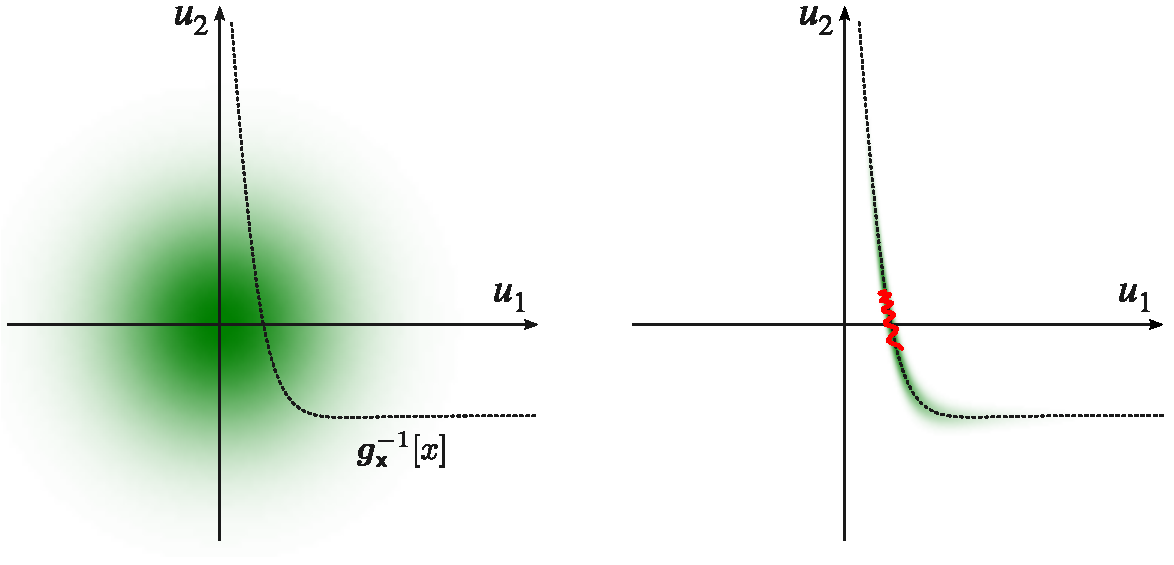
\includegraphics[width=0.8\textwidth]{images/gaussian-abc-with-hmc-trajectory-gray}
\caption[Oscillatory Hamiltonian trajectory example.]{Illustration of oscillatory behaviour in \ac{HMC} trajectories when using an \ac{ABC} target density \eqref{eq:abc-density-input-space} in the input space to a generative model. The left axis shows the two-dimensional input space $\set{U}$ of a toy differentiable generative model with a Gaussian input density $\rho$ (green shading). The dashed curve shows the one-dimensional manifold corresponding to the fibre under the generator function $\genfunc_{\rvar{x}}$ of an observed output $x$. The right axis shows the same input space with now the green shading showing the density proportional to $k_\epsilon\lpa x\gvn \genfunc_{\rvar{x}}(\vct{u})\rpa \,\rho(\vct{u})$ with a Gaussian $k_\epsilon$. The red curve shows a simulated \ac{HMC} trajectory using this density as the target: the large magnitude density gradients normal to the manifold cause high-frequency oscillations and slows movement along the manifold (which corresponds to variation in the latent variable $\rvar{z}$).}
\label{fig:gaussian-abc-hmc-trajectory-example}
\end{figure} 

There is a direct link between the reparameterisation of a generative model used here to allow application of alternative \ac{MCMC} transition operators to \ac{ABC} inference and the reparameterisation of the density estimators used in pseudo-marginal \ac{MCMC} methods proposed in Chapter \ref{ch:pseudo-marginal-methods}. For the common special case (and typical \ac{ABC} setting) of a directed generative model with a tractable marginal density on the unobserved variables $\pden{\rvct{z}}$, we have that
\begin{align}\label{eq:abc-expectation-input-space-directed}
  &\expc{f(\rvct{z}) \gvn \rvct{y}=\vct{y};\,\epsilon} = \\ \nonumber
  &\qquad
  \frac{1}{\pden{\rvct{y}}(\vct{y})}
  \int_\set{Z}\int_{\set{U}_2} 
    f(\vct{z}) \,
    k_\epsilon{\lpa\vct{y};\,\genfunc_{\rvct{x}|\rvct{z}}(\vct{z},\,\vct{u}_2)\rpa}\,
    \pden{\rvct{z}}(\vct{z})
    \rho_2(\vct{u}_2)
  \,\dr\vct{u}_2\,\dr\vct{z}
\end{align}
and so the target density for inference is
\begin{equation}\label{eq:abc-density-input-space-directed}
  \pi_\epsilon(\vct{z},\vct{u}_2) = \frac{1}{\pden{\rvct{y}}(\vct{y})} 
  k_\epsilon{\lpa\vct{y}\gvn\genfunc_{\rvct{x}|\rvct{z}}(\vct{z},\,\vct{u}_2)\rpa}\,\pden{\rvct{z}}(\vct{z})\,\rho_2(\vct{u}_2).
\end{equation}
Identifying $Z = \pden{\rvct{y}}(\vct{y})$, $\esttgtdens(\vct{z}, \vct{u}_2) = k_\epsilon{\lpa\vct{y}\gvn\genfunc_{\rvct{x}|\rvct{z}}(\vct{z},\,\vct{u}_2)\rpa}\,\pden{\rvct{z}}(\vct{z})$ and $\rho = \rho_2$, this has directly the same form as \eqref{eq:auxiliary-pm-target-density}. The main difference in the target density \eqref{eq:abc-density-input-space} is therefore that all of the random inputs, both those being used to generate the unobserved variables $\rvct{z}$ and to generate the observed variables $\rvct{x}$ given the unobserved variables, are treated equivalently. Although a minor difference, the formulation used in this Chapter helps clarify a geometric interpretation of the distribution induced in the input space to a generator when conditioning on observed values of its outputs which we will exploit in the following section.

%Jointly updating all the inputs $\rvct{u}$ to a directed generative can be advantageous compared to alternating updates of the unobserved variables $\rvct{z}$ and random inputs $\rvct{u}_2$ to $\genfunc_{\rvct{x}|\rvct{z}}$ when there are strong dependencies between the plausible values for $\rvct{u}_2$ and $\rvct{z}$.   
%This latter form is directly comparable to the reparameterisation suggested in \citep{murray2010slice}  for pseudo-marginal inference problems. There it is applied to construct a \ac{MCMC} method which uses slice sampling transition operators to iterate between updating the unobserved variables $\rvct{z}$ given random inputs $\rvct{u}_2$ and vice versa. For models in which the target density \eqref{eq:abc-density-input-space} is continuous with respect to both arguments, the slice sampling updates will be almost surely move the state a non-zero distance, therefore the chain will not `stick'. Related approaches using Metropolis updates instead have also been proposed \citep{dahlin2015accelerating,deligiannidis2015correlated}.

\section[Inference in differentiable generative models]{Asymptotically exact inference in \\ differentiable generative models}

In the reparameterising inference in terms of evaluating an integral over the input space we have still so far required the definition of a kernel $k_\epsilon$ and tolerance $\epsilon$ and the integral being estimated is the approximate expectation \eqref{eq:abc-expectation} rather than target conditional expectation $\expc{f(\rvct{z}) \gvn \rvct{x}\,}$ we are directly interested in. We now consider in the specific case of differentiable generative models how to perform inference without introducing an \ac{ABC} kernel.

%Although reparameterising the \ac{ABC} expectation as an integral over the input space and performing inference in that space can in itself sign
%Now considering specifically differentiable generative models and returning to the general case where the model is not necessarily directed. 
We begin an initial intuition for the approach, by considering taking the limit of $\epsilon \to 0$ in the integral \eqref{eq:abc-expectation-input-space} corresponding to evaluating the \ac{ABC} conditional expectation in the generator input space. We previously showed in \eqref{eq:abc-expectation-limit} that the approximate expectation $\expc{f(\rvct{z}) \gvn \rvct{y}= \vct{y};\,\epsilon}$ converges as $\epsilon \to 0$ to the conditional expectation of interest $\expc{f(\rvct{z}) \gvn \rvct{x} = \vct{y}}$, providing that the implicit distribution of the observed variables in the generative model $\prob{\rvct{x}}$ is absolutely continuous with respect to the Lebesgue measure with density $\pden{\rvct{x}}$. Informally for kernels meeting the conditions \eqref{eq:abc-valid-kernel-condition-1} and \eqref{eq:abc-valid-kernel-condition-2}, in the limit of $\epsilon \to 0$ the kernel density $k_\epsilon\lpa{\vct{y}};\,\genfunc_{\rvct{x}}(\vct{u})\rpa$ tends to a Dirac delta ${\delta}\lpa\vct{y} - \genfunc_{\rvct{x}}(\vct{u})\rpa$ and so
\begin{align}\label{eq:expectation-input-space-limit}
  \expc{f(\rvct{z}) \gvn \rvct{x}=\vct{y}} &=
  \lim_{\epsilon\to 0}  \expc{f(\rvct{z}) \gvn \rvct{y}=\vct{y};\,\epsilon} 
  \\
  &\simeq
  \frac{
  \int_{\set{U}} 
    f\circ\genfunc_{\rvct{z}}(\vct{u}) \,
    \delta\lpa\vct{y} - \genfunc_{\rvct{x}}(\vct{u})\rpa\,
    \rho(\vct{u})
  \,\dr\vct{u}
  }
  {
    \int_{\set{U}} 
    \delta\lpa\vct{y} - \genfunc_{\rvct{x}}(\vct{u})\rpa\,
    \rho(\vct{u})
  \,\dr\vct{u}
  }.
\end{align}
%  \\
%  &\propto
%  \int_{\set{U}} 
%    f\,\circ\,\genfunc_{\rvct{z}}(\vct{u}) \,
%    {\delta}\lpa{\vct{y}} - \genfunc_{\rvct{x}}(\vct{u})\rpa\,
%    \rho(\vct{u})
%  \,\dr\vct{u}.
The Dirac delta term restricts the integral across the input space $\set{U}$ to an embedded, $M - N_{\rvct{x}}$ dimensional, implicitly-defined manifold corresponding to the fibre of $\vct{y}$ under $\genfunc_{\rvct{x}}$, $\preimage{\genfunc_{\rvct{x}}}{\vct{y}} \equiv \fset{\vct{u} \in \set{U} :  \genfunc_{\rvct{x}}(\vct{u}) = \vct{y}}$. It is not necessarily immediately clear however how to define the required density on that manifold for abitrary non-injective $\genfunc_{\rvct{x}}$.

In differentiable generative models we can however use a derivation equivalent to that given by Diaconis, Holmes and Shahshahani in \citep{diaconis2013sampling} for the conditional density on a manifold to find an expression for the conditional expectation consistent with definition given in \eqref{eq:conditional-expectation-property}. %Our derivation is largely a restatement of the results in \citep{diaconis2013sampling} except for the minor difference of working in terms of conditional expectations rather densities. % (with the motivation that the conditional expectation is object we are directly interested in).%; we provide the derivation mainly for completeness and to make it more easily relatable to our notation.
The key result we use is a formula from geometric measure-theory, Federer's \emph{co-area formula} \citep[\S 3.2.12]{federer2014geometric}. This generalises Fubini's theorem for iterated integrals on spaces defined by a Cartesian product to more general foliations of a space.% that we earlier used implicitly when deriving the \ac{ABC} conditional expectation in \eqref{eq:abc-conditional-expectation-derivation} to cases where the iterated integrals
\begin{theorem}[Co-area formula]\label{thm:co-area-formula}
\marginpar{The $K$-dimensional Hausdorff measure $\haum{K}$ on $\reals^N$ for $K \in \naturals$, $0 < K < N$ formalises a measure of the `volume' of $K$-dimensional submanifolds of $\reals^N$ - e.g. for $K=1$ it corresponds to the length of a curve in $\reals^N$. Additionally $\haum{N} = \lebm{N}$ and $\haum{{\scriptstyle 0}} = \countm$.}
Let $\set{V} \subseteq \reals^L$ and $\set{W} \subseteq \reals^K$ with $L \geq K$, $\vctfunc{m}:\set{V}\to\set{W}$ be Lipschitz and $\func{h} : \set{V} \to \reals$ be Lebesgue measurable. Then
\begin{equation}\label{eq:co-area-formula}
    \int_{\set{V}} 
      \func{h}(\vct{v}) \, \jacobproddet{\vctfunc{m}}{\vct{v}}
    \,\dr\lebm{L}(\vct{v})
    = 
    \int_{\set{W}}
      \int_{\preimage{\vctfunc{m}}{\vct{w}}} \func{h}(\vct{v}) \,\dr\haum{L-K}(\vct{v})
    \,\dr\lebm{K}(\vct{w})
\end{equation}
with $\haum{L-K}$ denoting the $L-K$-dimensional Hausdorff measure and $\jacobproddet{\vctfunc{m}}{\vct{v}}$ denoting the generalised Jacobian determinant
\begin{equation}\label{eq:jacobian-product-det}
  \jacobproddet{\vctfunc{m}}{\vct{v}} \equiv 
  \left|\,\jacob{\vctfunc{m}}{\vct{u}}\jacob{\vctfunc{m}}{\vct{u}}\tr\right|^{\frac{1}{2}}.
\end{equation}
%$\preimage{\vctfunc{m}}{\vct{w}}$ denoting the preimage of $\lbrace \vct{w} \rbrace$ under the map $\vctfunc{m}$ i.e. 
%\begin{equation}\label{eq:preimage-notation-definition}
%  \preimage{\vctfunc{m}}{\vct{w}} \equiv 
%  \fset{\vct{v} \in \set V : \vctfunc{m}(\vct{v}) = \vct{w}}.
%\end{equation}
\end{theorem}
More immediately applicable in our case is the following corollary.
\begin{corollary}\label{col:co-area-formula}
If $Q$ is a probability measure on $\set{V}$ with density $q$ with respect to the Lebesgue measure $\lambda^L$ and $\jacobian{\vctfunc{m}}$ is full row-rank $Q$-almost everywhere, then for Lebesgue measurable $\func{h}' : \set{V} \to \reals$
\begin{equation}\label{eq:co-area-formula-corollary}
\begin{split}
    &\int_{\set{V}} 
      \func{h}'(\vct{v})\,q(\vct{v})
    \,\dr\lebm{L}(\vct{v})
    =\,\\
    &\qquad
    \int_{\set{W}}
      \int_{\preimage{\vctfunc{m}}{\vct{w}}}
        \func{h}'(\vct{v}) \,
        q(\vct{v})\,
        \jacobproddet{\vctfunc{m}}{\vct{v}}^{-1}
      \,\dr\haum{L-K}(\vct{v})
    \,\dr\lebm{K}(\vct{w}).
\end{split}
\end{equation}
\end{corollary}
This can be shown by setting $h(\vct{v}) = h'(\vct{v})\,q(\vct{v})\jacobproddet{\vctfunc{f}}{\vct{v}}^{-1}$ in \eqref{eq:co-area-formula} and using the equivalence of Lebesgue integrals in which the integrand differs only zero-measure sets. 

We first show that $\prob{\rvct{x}}$ has a density $\pden{\rvct{x}} = \td{\prob{\rvct{x}}}{\lebm{N_{\rvct{x}}}}$.

\begin{proposition}[Change of variables in a differentiable generative model]\label{prop:change-of-variables-in-dgm}
For a differentiable generative model $(\set{U},\sset{F}\kern-2pt,\rho,\mu,\genfunc_{\rvct{x}},\genfunc_{\rvct{z}})$ as defined in Definition \ref{def:differentiable-generative-model}, then if the generator $\genfunc_{\rvct{x}}$ is Lipschitz and the Jacobian $\jacobian{\genfunc_{\rvct{x}}}$ has full row-rank $\prob{\rvct{u}}$-almost everywhere, the observed vector $\rvct{x}$ has a density with respect to the Lebesgue measure satisfying
\begin{equation}\label{eq:dgm-marginal-density-x}
  \pden{\rvct{x}}({\vct{x}})  =
  \int_{\preimage{\genfunc_{\rvct{x}}}{\vct{x}}}
    \rho(\vct{u})\,
    \jacobproddet{\genfunc_{\rvct{x}}}{\vct{u}}^{-1}
  \,\dr\haum{M-N_{\rvct{x}}}(\vct{u})
  \qquad \forall \vct{x} \in\set{X}.
\end{equation}
%with $\genfunc_{\rvct{x}}^{-1}[\vct{x}] = \fset{\vct{u} \in \set{U} : \genfunc_{\rvct{x}}(\vct{u}) = \vct{x}}$.
\end{proposition}
\begin{proof}
From Definition \ref{def:differentiable-generative-model} we have that $\rvct{x} = \genfunc_{\rvct{x}}(\rvct{u})$ and $\td{\prob{\rvct{u}}}{\lebm{M}} = \rho$ and so
\begin{equation*}
  \prob{\rvct{x}}(\set{A}) 
  =
  \int_{\set{U}} 
    \ind{\set{A}}\circ\,\genfunc_{\rvct{x}}(\vct{u})\,\rho(\vct{u})
  \,\dr\lebm{M}(\vct{u})
  \qquad \forall \set{A} \in\sset{G}.
\end{equation*}
As $\genfunc_{\rvct{x}}$ is Lipschitz and $\jacobian{\genfunc_{\rvct{x}}}$ has full row-rank $\prob{\rvct{u}}$-almost everywhere we can apply Corollary \ref{col:co-area-formula}, and so we have that $\forall \set{A} \in\sset{G}$
\begin{equation*}
  \prob{\rvct{x}}(\set{A}) =
  \int_{\set{X}}
  \int_{\preimage{\genfunc_{\rvct{x}}}{\vct{x}}}\kern-1pt
    \ind{\set{A}}\!\circ\,\genfunc_{\rvct{x}}(\vct{u})\,\rho(\vct{u})\,
    \jacobproddet{\genfunc_{\rvct{x}}}{\vct{u}}^{-1}
  \,\dr\haum{M-{N_{\rvct{x}}}}(\vct{u})
  \,\dr\lebm{N_{\rvct{x}}}(\vct{x}).
\end{equation*}
The term $\ind{\set{A}}\!\circ\,\genfunc_{\rvct{x}}(\vct{u})$ inside the inner integral is equal to $\ind{\set{A}}(\vct{x})$ across all points in the fibre $\preimage{\genfunc_{\rvct{x}}}{\vct{x}}$ being integrated across and so can be taken outside the inner integral to give
\begin{align*}
  \prob{\rvct{x}}(\set{A})
  &=
  \int_{\set{X}}
  \ind{\set{A}}(\vct{x})
  \int_{\preimage{\genfunc_{\rvct{x}}}{\vct{x}}} 
   \rho(\vct{u})\,
   \jacobproddet{\genfunc_{\rvct{x}}}{\vct{u}}^{-1}
  \,\dr\haum{M-{N_{\rvct{x}}}}(\vct{u})
  \,\dr\lebm{N_{\rvct{x}}}(\vct{x})\\
  &=
  \int_{\set{A}}
  \int_{\preimage{\genfunc_{\rvct{x}}}{\vct{x}}} 
   \rho(\vct{u})\,
   \jacobproddet{\genfunc_{\rvct{x}}}{\vct{u}}^{-1}
  \,\dr\haum{M-{N_{\rvct{x}}}}(\vct{u})
  \,\dr\lebm{N_{\rvct{x}}}(\vct{x}).
\end{align*}
By definition the density $\pden{\rvct{x}}$ of a probability measure $\prob{\rvct{x}}$ with respect to the Lebesgue measure $\lebm{N_{\rvct{x}}}$ satisfies
\begin{equation*}
  \prob{\rvct{x}}(\set{A}) = \int_{\set{A}} \pden{\rvct{x}}(\vct{x}) \,\dr\lebm{N_{\rvct{x}}}(\vct{x})
  \qquad \forall \set{A} \in \sset{G}
\end{equation*}
$\therefore$ $\prob{\rvct{x}}$ has a density corresponding to \eqref{eq:dgm-marginal-density-x} with respect to $\lebm{N_{\rvct{x}}}$. \qedhere
\end{proof}
This is a generalisation of the change of variables formula under a diffeomorphism encountered previously in Chapter \ref{ch:probabilistic-modelling}. We now derive a result for the conditional expectation.
\begin{proposition}[Conditional expectations in a differentiable \\generative model]\label{prop:conditional-expectations-in-dgm}
For a differentiable generative model $(\set{U},\sset{F}\kern-2pt,\rho,\mu,\genfunc_{\rvct{x}},\genfunc_{\rvct{z}})$ as defined in Definition \ref{def:differentiable-generative-model} and satisfying the conditions in Proposition \ref{prop:change-of-variables-in-dgm}, then for Lebesgue measurable functions $f : \set{X} \to \reals$ and $\vct{x} \in \set{X}$ such that $\pden{\rvct{x}}(\vct{x}) > 0$ we have that
\begin{equation}\label{eq:cond-expectation-input-space}
\begin{split}
  &\expc{f(\rvct{z}) \gvn \rvct{x}=\vct{x}}
  =\,\\
  &\qquad\qquad
  \frac{1}{\pden{\rvct{x}}({\vct{x}})}
  \int_{\preimage{\genfunc_{\rvct{x}}}{\vct{x}}}
    f\circ\genfunc_{\rvct{z}}(\vct{u}) \, \rho(\vct{u}) \,
    \jacobproddet{\genfunc_{\rvct{x}}}{\vct{u}}^{-1}
  \,\dr\haum{M-N_{\rvct{x}}}(\vct{u}).
\end{split}
\end{equation}
%with $\set{C} = \fset{\vct{u} \in \set{U} :  \genfunc_{\rvct{x}}(\vct{u}) = \vct{x}}$.
\end{proposition}
\begin{proof}
Restating the general definition for a conditional expectation from Chapter \ref{ch:probabilistic-modelling}, we need to find a measurable function $\expc{f(\rvct{z}) \gvn \rvct{x}\,} : \set{X} \to \reals$ which $\forall\set{A} \in \sset{G}$ satisfies
\begin{equation*}
  \int_{\set{A}}
    \expc{f(\rvct{z}) \gvn \rvct{x} = \vct{x}} 
  \,\dr\prob{\rvct{x}}(\vct{x}) =
  \int_{\set{A} \times \set{Z}}
    f(\vct{z}) 
  \,\dr\prob{\rvct{x},\rvct{z}}(\vct{x},\vct{z}),
\end{equation*}
with this uniquely defining the conditional expectation up to $\prob{\rvct{x}}$-null sets. Using $\rvct{x} = \genfunc_{\rvct{x}}(\rvct{u})$, $\rvct{z} = \genfunc_{\rvct{z}}(\rvct{u})$ and $\pden{\rvct{u}} = \rho$ we have that $\forall\set{A} \in \sset{G}$
\begin{equation*}
  \int_{\set{A} \times \set{Z}}
    f(\vct{z}) 
  \,\dr\prob{\rvct{x},\rvct{z}}(\vct{x},\vct{z}) =
  \int_{\set{U}}
  \ind{\set{A}}\circ\,\genfunc_{\rvct{x}}(\vct{u})\,
  f\circ\genfunc_{\rvct{z}}(\vct{u})\,
  \rho(\vct{u})
  \,\dr\lebm{M}(\vct{u}).
\end{equation*}
Applying the co-area corollary \eqref{eq:co-area-formula-corollary} to the right-hand side and again noting the indicator term $\ind{\set{A}}\circ\,\genfunc_{\rvct{x}}(\vct{u})$ is constant across the fibre being integrated on, we have that $\forall \set{A} \in\sset{G}$
\begin{align*}
  &\int_{\set{A} \times \set{Z}}
    f(\vct{z}) 
  \,\dr\prob{\rvct{x},\rvct{z}}(\vct{x},\vct{z})\\
  &=
  \int_{\set{X}} \int_{\preimage{\genfunc_{\rvct{x}}}{\vct{x}}}
   \ind{\set{A}}\circ\,\genfunc_{\rvct{x}}(\vct{u})\,
   f\circ\genfunc_{\rvct{z}}(\vct{u})\,
   \rho(\vct{u})\,
   \jacobproddet{\genfunc_{\rvct{x}}}{\vct{u}}^{-1}
  \,\dr\haum{M-{N_{\rvct{x}}}}(\vct{u})
  \,\dr\lebm{N_{\rvct{x}}}(\vct{x})
  \\
  &=
  \int_{\set{A}}
  \int_{\preimage{\genfunc_{\rvct{x}}}{\vct{x}}}\kern-1pt
   f\circ\genfunc_{\rvct{z}}(\vct{u})\,
   \rho(\vct{u})\,
   \jacobproddet{\genfunc_{\rvct{x}}}{\vct{u}}^{-1}
  \,\dr\haum{M-{N_{\rvct{x}}}}(\vct{u})
  \,\dr\lebm{N_{\rvct{x}}}(\vct{x}).
\end{align*}
Finally using that $\prob{\rvct{x}}$ has a density $\pden{\rvct{x}}$ with respect to the Lebesgue measure as shown in the previous proposition, we have that
\begin{equation*}
\begin{split}
  &\int_{\set{A} \times \set{Z}}
    f(\vct{z}) 
  \,\dr\prob{\rvct{x},\rvct{z}}(\vct{x},\vct{z}) =\,\\
  &\qquad
  \int_{\set{A}}
  \frac{1}{\pden{\rvct{x}}(\vct{x})}
  \int_{\preimage{\genfunc_{\rvct{x}}}{\vct{x}}}\kern-1pt
   f\circ\genfunc_{\rvct{z}}(\vct{u})\,
   \rho(\vct{u})\,
   \jacobproddet{\genfunc_{\rvct{x}}}{\vct{u}}^{-1}
  \,\dr\haum{M-{N_{\rvct{x}}}}(\vct{u})
  \,\dr\prob{\rvct{x}}(\vct{x}).
\end{split}
\end{equation*}
Note that as we are integrating against the probability measure $\prob{\rvct{x}}$ we can safely ignore the points for which $\pden{\rvct{x}}(\vct{x}) = 0$ as the set of all such points naturally has zero measure under $\prob{\rvct{x}}$ and so does not contribute to integral. Comparing to the definition of the conditional expectation we have that \eqref{eq:cond-expectation-input-space} satisfies the definition. \qedhere
\end{proof}

%By applying the the \emph{Co-Area Formula} \citep[\S 3.2.12]{federer2014geometric} the integral with respect to the Lebesgue measure across $\set{U}$ in \eqref{eq:expectation-input-space-limit} can be rewritten as integral across the embedded manifold $\set{C}$ with respect the Hausdorff measure for the manifold
The expression derived for the conditional expectation has the form of an integral of function $f \circ \genfunc_{\rvct{z}}$ integrated against a density
\begin{equation}\label{eq:tgt-density-on-manifold}
    \pi(\vct{u}) =
    \frac{1}{\pden{\rvct{x}}(\vct{x})}\,
    \jacobproddet{\genfunc_{\rvct{x}}}{\vct{u}}^{-1}\,
    \rho(\vct{u}) 
\end{equation}
which we can evaluate up to an unknown normalising constant $\pden{\rvct{x}}(\vct{x})$. The key complicating factor is that the integral is now not across a Euclidean space, but an implictly defined manifold corresponding to the fibre $\preimage{\genfunc_{\rvct{x}}}{\vct{x}}$. However if we can construct a Markov transition operator which has an invariant distribution with density \eqref{eq:tgt-density-on-manifold} with respect to the Hausdorff measure on the manifold, then we can use samples of the chain states $\lbrace\rvct{u}^{(s)}\rbrace_{s=1}^S$ to compute an estimate
\begin{equation}\label{eq:mc-est-cond-expc}
    \hat{\rvar{f}}_S =
    \frac{1}{S} 
    \sum_{s=1}^S \lpa
      \func{f}\,\circ\,\genfunc_{\rvct{z}}\lpa\rvct{u}^{(s)}\rpa
    \rpa
\end{equation}
which providing the chain is also aperiodic and irreducible will be a consistent estimator for $\expc{f(\rvct{z}) \gvn \rvct{x} = \vct{x}}$. Although constructing a Markov transition operator with the required properies is non-trivial, there is a significant body of existing work on methods for defining Markov chains on manifolds. We propose here to use a constrained Hamiltonian Monte Carlo method.

\section{Constrained Hamiltonian Monte Carlo}\label{sec:chmc}

The \ac{HMC} method introduced in Chapter \ref{ch:approximate-inference} defined a transition operator which left target distributions on a Euclidean space invariant. In our case the target distribution is defined on an implicitly defined manifold $\preimage{\genfunc_{\rvct{x}}}{\vct{x}}$ embedded in a Euclidean space $\set{U}=\reals^M$. Intuitively we can consider the manifold as representing the allowable configurations of mechanical system subject to a constraint. By simulating a constrained Hamiltonian dynamic we can therefore construct a \ac{HMC} transition operator analagous to those discussed in Chapter \ref{ch:approximate-inference} but that generates chains on an implicitly defined manifold rather than an unconstrained Euclidean space.

The use of constrained Hamiltonian dynamics within a \ac{MCMC} method has been proposed by multiple authors. In the molecular dynamics literature, Hartmann and Schutte \citep{hartmann2005constrained} and Leli{\`e}vre, Rousset and Stoltz \citep{lelievre2012langevin} used simulated constrained Hamiltonian dynamics within a \ac{HMC} framework to estimate free-energy profiles of molecular systems. Most relevantly for our case, Brubaker, Salzmann and Urtasun \citep{brubaker2012family} proposed a constrained \ac{HMC} algorithm for performing inference in target distributions defined on implicitly defined embedded manifolds. We will concentrate on the algorithm proposed in \citep{brubaker2012family} here. %As well  and give detailed statements of sufficient conditions for the constructed chains to converge to generating samples from the target distribution.

To simplify notation and emphasise the generality of the approach beyond our specific setting, we define the following notation for the vector \emph{constraint function} on the system and corresponding Jacobian
\begin{equation}\label{eq:constraint-def}
  \vctfunc{c}(\vct{u}) = \genfunc_{\rvct{x}}(\vct{u}) - \vct{x},
  \qquad
  \jacob{\vctfunc{c}}{\vct{u}} = \jacob{\genfunc_{\rvct{x}}}{\vct{u}}.
\end{equation}
The \emph{constraint manifold} is then defined as the zero level-set of $\vctfunc{c}$, in our case corresponding to the fibre of $\vct{x}$ under the generator $\genfunc_{\rvct{x}}$
\begin{equation}\label{eq:constraint-manifold-def}
  \set{C} = \lbrace \vct{u} \in \reals^M : \vctfunc{c}(\vct{u}) = \vct{0} \rbrace =
  \preimage{\genfunc_{\rvct{x}}}{\vct{x}}.
\end{equation}
Defining as in Chapter \ref{ch:approximate-inference} the potential energy $\phi$ as the negative logarithm of the unnormalised target density and the kinetic energy as a quadratic form $\frac{1}{2}\vct{p}\tr\mtx{M}^{-1}\vct{p}$ where $\vct{p}$ is a vector of momenta, the Hamiltonian for the constrained system can be written as
\begin{equation}\label{eq:constrained-hamiltonian}
    \hamiltonian(\vct{u}, \vct{p}) = 
    \phi(\vct{u}) + \frac{1}{2}\vct{p}\tr\mtx{M}^{-1}\vct{p}
    + \vctfunc{c}(\vct{u})\tr\vct{\lambda},
\end{equation}
where $\vct{\lambda}$ is a vector of Lagrangian multipliers for the constraints. The constrained Hamiltonian dynamic is then defined by
\begin{equation}\label{eq:constrained-hamiltonian-dynamic}
    \td{\vct{u}}{t} = \mtx{M}^{-1}\vct{p},
    ~~
    \td{\vct{p}}{t} = -\grad{\phi}{\vct{u}}\tr - \jacob{\vctfunc{c}}{\vct{u}}\tr\vct{\lambda},
\end{equation}
with the Lagrange multipliers taking values to ensure the system constraints are satisfied. In addition to the configuration constraint $\vctfunc{c}\lpa\vct{u}\rpa = \vct{0}$ there is a corresponding implied constraint on the momenta $\vct{p}$ requiring that the configuration velocity $\mtx{M}^{-1}\vct{p}$ is always tangential to the constraint manifold at the current configuration, or equivalently that the momenta are in the \emph{tangent space} to the constraint manifold. The tangent space $\sset{T}_{\vct{u}}\set{C}$ at a configuration $\vct{u}$ is defined as
\begin{equation}\label{eq:constraint-tanget-space}
  \sset{T}_{\vct{u}}\set{C} = \lbr \vct{p} \in \reals^M : \jacob{\vctfunc{c}}{\vct{u}}\mtx{M}^{-1}\vct{p} = \vct{0} \rbr.
\end{equation}
The complete set of valid configuration--momentum state pairs is termed the \emph{tangent bundle} $\sset{T}\set{C}$ of the constraint manifold and defined as
\begin{equation}\label{eq:constraint-tanget-bundle}
  \sset{T}\set{C} = \lbr 
    \vct{u},\vct{p} \in \reals^M \times \reals^M :
    \vctfunc{c}(\vct{u}) = \vct{0},~
    \jacob{\vctfunc{c}}{\vct{u}}\mtx{M}^{-1}\vct{p} = \vct{0} 
  \rbr.
\end{equation}
The solution at time $t$ to the initial value problem defined by the \acp{ODE} \eqref{eq:constrained-hamiltonian-dynamic} defines a flow map $\cflowmap_t : \sset{T}\set{C} \to \sset{T}\set{C}$ between states in the tangent bundle of the constraint manifold. As with the unconstrained Hamiltonian dynamics encountered previously in Chapter \ref{ch:approximate-inference}, this flow map exactly conserves the Hamiltonian and is time-reversible. Further the flow map of the constrained dynamic is symplectic and  conserves the volume element of the constraint manifold tangent bundle \citep{leimkuhler2004simulating}.

Importantly there exist symplectic integrators which can be used to approximate the constrained Hamiltonian dynamic flow map and which map between states exactly in the constraint manifold tangent bundle (modulo numerical error due to finite precision arithmetic). The approximate flow maps defined by these integrators are time-reversible and conserve the tangent bundle volume element. They also exhibit the bounded change in the Hamiltonian over simulated trajectories discussed previously for the unconstrained case in Chapter \ref{ch:approximate-inference}.

A popular symplectic numerical integrator for constrained Hamiltonian dynamics is the RATTLE method \citep{andersen1983rattle,leimkuhler1994symplectic}. This a generalisation of the leapfrog integrator encountered in our previous discussion of \ac{HMC} in Chapter \ref{ch:approximate-inference} with additional steps to project the states on to the tangent bundle of the constraint manifold. A RATTLE step is composed of three component maps. The first map is defined by
\begin{equation}\label{eq:rattle-step-a}
\begin{split}
  &\hat{\cflowmap}_{\delta t}^{\textsc{a}}(\vct{u},\vct{p}) =
  \lpa \vct{u} + \delta t \mtx{M}^{-1}(\vct{p}-\jacob{\vctfunc{c}}{\vct{u}}\tr\vct{\lambda}),\,\vct{p}-\jacob{\vctfunc{c}}{\vct{u}}\tr\vct{\lambda}\rpa\\
  &\qquad\textrm{solving for}~\vct{\lambda}~\textrm{such that}~\vctfunc{c}\lpa \vct{u} + \delta t \mtx{M}^{-1}(\vct{p}-\jacob{\vctfunc{c}}{\vct{u}}\tr\vct{\lambda})\rpa = \vct{0}.
\end{split}
\end{equation}
This defines an approximate \emph{geodesic} step on the constraint manifold: the configuration $\vct{u}$ is incremented in the direction of the current velocity $\mtx{M}^{-1}\vct{p}$ and then the new configuration state projected back on to the constraint manifold by solving a non-linear system of equations for the Lagrange multipliers $\vct{\lambda}$. %After appying $\cflowmap^{\textsc{a}}_{\delta t}$ the updated configuration will be on the constraint manifold, but the updated momentum will no longer be in the tangent space to constraint manifold at the updated configuration.

The second component map updates the momenta with a `kick' in the direction of the potential energy gradient
\begin{equation}\label{eq:rattle-step-b}
  \hat{\cflowmap}^{\textsc{b}}_{\delta t}(\vct{u},\vct{p}) =
  \lpa \vct{u},\,\vct{p}-\delta t \grad{\phi}{\vct{u}}\tr \rpa.
\end{equation}
Though both $\hat{\cflowmap}_{\delta t}^{\textsc{a}}$ and $\hat{\cflowmap}^{\textsc{b}}_{\delta t}$ steps will map between configurations in the constraint manifold (trivially in the case of $\hat{\cflowmap}^{\textsc{b}}_{\delta t}$ as the configurations are kept fixed), the corresponding momenta will not be confined to the tangent spaces to the manifold. The final component map projects the momenta in to the tangent space of the constraint manifold at the current configuration. It is defined by
\begin{equation}
\begin{split}
  &\hat{\cflowmap}^{\textsc{p}}(\vct{u},\vct{p}) =
  \lpa \vct{u},\,\vct{p}-\jacob{\vctfunc{c}}{\vct{u}}\tr\vct{\lambda}\rpa\\
  &\qquad\textrm{solving for}~\vct{\lambda}~\textrm{such that}~\jacob{\vctfunc{c}}{\vct{u}}\mtx{M}^{-1}(\vct{p}-\jacob{\vctfunc{c}}{\vct{u}}\tr\vct{\lambda}) = \vct{0}.
\end{split}
\end{equation}
In this case the system of equation needing to be solved is linear and has an analytic solution, giving the following closed-form definition
\begin{equation}\label{eq:rattle-step-p}
  \hat{\cflowmap}^{\textsc{p}}(\vct{u},\vct{p}) =
  \lpa \vct{u},\,\vct{p}-\jacob{\vctfunc{c}}{\vct{u}}\tr(\jacob{\vctfunc{c}}{\vct{u}}\mtx{M}^{-1}\jacob{\vctfunc{c}}{\vct{u}}\tr)^{-1}\jacob{\vctfunc{c}}{\vct{u}}\mtx{M}^{-1}\vct{p}\rpa.
\end{equation}
An overall RATTLE step is then defined by the composition
\begin{equation}\label{eq:rattle-ste}
  \hat{\cflowmap}^{\textsc{r}}_{\delta t} =
  \hat{\cflowmap}^{\textsc{p}} \circ
  \hat{\cflowmap}^{\textsc{b}}_{\frac{\delta t}{2}} \circ
  \hat{\cflowmap}^{\textsc{p}} \circ
  \hat{\cflowmap}_{\delta t}^{\textsc{a}} \circ
  \hat{\cflowmap}^{\textsc{p}} \circ
  \hat{\cflowmap}^{\textsc{b}}_{\frac{\delta t}{2}}
  .
\end{equation}
In practice the intermediate momentum projection steps $\hat{\cflowmap}^{\textsc{p}}$ are redundant \citep{mclachlan2014geometric} and so typically the momentum is only projected back in to the tangent space at the end of the step, giving the following update 
\begin{equation}\label{eq:rattle-step-alt}
  \hat{\cflowmap}^{\textsc{r}}_{\delta t} =
  \hat{\cflowmap}^{\textsc{p}} \circ
  \hat{\cflowmap}^{\textsc{b}}_{\frac{\delta t}{2}} \circ
  \hat{\cflowmap}_{\delta t}^{\textsc{a}} \circ
  \hat{\cflowmap}^{\textsc{b}}_{\frac{\delta t}{2}}.
\end{equation}
Solving the non-linear constraint equations in the geodesic step $\hat{\cflowmap}_{\delta t}^{\textsc{a}}$ is computationally challenging, with closed form solutions generally not available and so an iterative approach required. Further the system of equations are not guaranteed to have a unique solution: if the step size $\delta t$ is too large there can be multiple or no solutions \citep{leimkuhler2004simulating}. It is important therefore to keep the step size small enought to avoid the iterative solver converging to an incorrect solution or not converging at all. Often the resulting step size will be smaller than required however in terms of controlling the Hamiltonian error over a simulated trajectory. An alternative to the standard RATTLE integrator is therefore to perform $N_g > 1$ inner geodesic steps $\hat{\cflowmap}_{\frac{\delta t}{N_g}}^{\textsc{a}}$ for each outer pair of momentum kick steps $\hat{\cflowmap}^{\textsc{b}}_{\frac{\delta t}{2}}$
\begin{equation}\label{eq:geodesic-integrator-step}
  \hat{\cflowmap}^{\textsc{g}}_{\delta t} =
  \hat{\cflowmap}^{\textsc{p}} \circ
  \hat{\cflowmap}^{\textsc{b}}_{\frac{\delta t}{2}} \circ
  \big(
  \hat{\cflowmap}^{\textsc{p}} \circ
  \hat{\cflowmap}_{\frac{\delta t}{N_g}}^{\textsc{a}}
  \big)^{N_g} \circ
  \hat{\cflowmap}^{\textsc{p}} \circ
  \hat{\cflowmap}^{\textsc{b}}_{\frac{\delta t}{2}}.
\end{equation}
This \emph{geodesic integrator} \citep{leimkuhler1996symplectic,leimkuhler2016efficient} scheme can reduce the number of potential energy gradient evaulations required by using a larger step size for the momentum kick updates while still maintaining a sufficiently small step size to avoid convergence issues in the geodesic step. %As with RATTLE the intermediate momentum projection steps $\hat{\cflowmap}^{\textsc{p}}$ can be neglected, though in practice we have found that they help to improve numerical stability and add minimal overhead.

Assuming the iterative solving of the projections to constraint manifold in the geodesic steps converge correctly, the approximate flow map defined by iterating RATTLE or geodesic integrator steps preserves the volume element of $\sset{T}\set{C}$ and is reversible under negation of the momenta. We can therefore use the composition of the approximate flow map with a momentum reversal operator to define a volume-preserving involution between states in $\sset{T}\set{C}$. We can then use this involution as a proposal generating mechanism for a Metropolis accept step \eqref{eq:metropolis-hastings-transition-deterministic-proposal} to correct for the Hamiltonian error in the approximate flow map. 

As in the standard \ac{HMC} algorithm, Metropolis updates with approximate flow map proposals are interleaved with updates in which the momenta are independently resampled. To ensure the momenta remain in the tangent space $\sset{T}_{\vct{u}}\set{C}$ to the constraint manifold after generating new values  from $\nrm{\vct{0},\mtx{M}}$, the momenta are projected in to the tangent space using the projection operator defined in \eqref{eq:rattle-step-p}. The overall constrained \ac{HMC} transition operator defined by this combination of momentum resampling and Metroplis accept step with a constrained dynamic proposal, leaves invariant the distribution with negative log density defined by the Hamiltonian in \eqref{eq:constrained-hamiltonian} on the constraint manifold tangent bundle $\sset{T}\set{C}$, and so marginally leaves the target distribution with density proportional to $\exp\lpa-\phi(\vct{u})\rpa$ on $\set{C}$ invariant.

%Although the properties of the approximate flow map are sufficient for ensuring the constrained \ac{HMC} transition operator leaves the target distribution on $\set{C}$ invariant, 
%Further conditions on the system are required to ensure ergodicity of chains generated by the transition operator. 
Ensuring ergodicity of chains generated by the constrained \ac{HMC} transition operator is in general more challenging than for \ac{HMC} on Euclidean spaces due to the often complex geometry of the constraint manifold $\set{C}$ and potential for numerical issues when solving the non-linear equations in the projection steps. In \citep{brubaker2012family} it is shown that if\footnote{We give only a loose statement of the full conditions here for brevity; for complete details see Theorems 1 to 4 in \citep{brubaker2012family}.}
\begin{itemize}
  \item $\set{C}$ is a connected, smooth differentiable manifold, 
  \item $\jacobian{\vctfunc{c}}$ has full row-rank everywhere, 
  \item and $\pi(\vct{u}) \propto \exp\lpa\phi(\vct{u})\rpa$ is smooth and strictly positive on $\set{C}$
\end{itemize}
for a constrained \ac{HMC} transition using an approximate flow map defined by a symplectic integrator with step size $\delta t$, if the step-size $\delta t$ is set sufficiently small such that there is a unique solution to the choice of Lagrange multipliers $\vct{\lambda}$ in each geodesic step \eqref{eq:rattle-step-a} and the iterative method employed converges to this solution in every step, that the overall transition operator will be irreducible, aperiodic and leave the target distribution on $\set{C}$ invariant.

These conditions put stricter requirements on the generator $\genfunc_{\rvct{x}}$ of a differentiable generative model than those specified in Definition \ref{def:differentiable-generative-model} and Proposition \ref{prop:conditional-expectations-in-dgm} if we wish to use a constrained \ac{HMC} method to estimate conditional expectations under the model. The requirement that $\set{C} = \preimage{\genfunc_{\rvct{x}}}{\vct{x}}$ is a smooth and connected manifold is likely to be challenging to check for complex generators. If the fibre of $\vct{x}$ under the generator $\genfunc_{\rvct{x}}$ consists of multiple disconnected components then the constrained Hamiltonian dynamic will remain confined to just one of them. Although problematic, this issue is similar to that faced by other \ac{MCMC} methods in target distributions with multiple separated modes. The requirement that the Jacobian $\jacobian{\genfunc_{\rvct{x}}}$ is defined and full row-rank everywhere is also stricter than previously required.

\begin{figure}[t]
\begin{subfigure}[b]{0.48\linewidth}
\centering
  \includetikz{preimage-manifold-example-hyperbola}
  \caption{$\preimage{\genfunc_{\rvar{x}}}{1}$}
  \label{sfig:disconnected-manifold-example-orig}
\end{subfigure}
\begin{subfigure}[b]{0.48\linewidth}
\centering
  \includetikz{preimage-manifold-example-hyperbolic-paraboloid}
  \caption{$\preimage{\genfunc_{\rvar{y}}}{1}$}
  \label{sfig:disconnected-manifold-example-noisy}
\end{subfigure}
\caption[Disconnected manifold example.]{Visualisations of the hyperbola fibre $\preimage{\genfunc_{\rvar{x}}}{1}$ of the toy generator $\genfunc_{\rvar{x}}$ defined in \eqref{eq:disconnected-manifold-example} consisting of two disconnected components and the corresponding connected hyperbolic paraboloid fibre $\preimage{\genfunc_{\rvar{y}}}{1}$ of the noisy generator.}
\label{fig:disconnected-manifold-example}
\end{figure}

If we define an augmented `noisy' generator
\begin{equation}
  \genfunc_{\rvct{y}}(\vct{u},\vct{n}) = \genfunc_{\rvct{x}}(\vct{u}) + \epsilon \vct{n}
\end{equation}
with $\vct{n} \sim \nrm{\vct{0},\mtx{I}}$ and $\epsilon$ a small positive constant, then if $\genfunc_{\rvct{x}}$ is differentiable everywhere then the Jacobian of the augmented generator $\jacobian{\genfunc_{\rvct{y}}}$ will be full row-rank everywhere. That $\jacobian{\genfunc_{\rvct{y}}}$ will have full-row rank everywhere is evident from its block structure $\jacob{\genfunc_{\rvct{y}}}{\vct{u},\vct{n}} = \lsb \jacob{\genfunc_{\rvct{x}}}{\vct{u}} \,\middle|\, \epsilon\idmtx \rsb$. The Jacobian being full row-rank implies that $\genfunc_{\rvct{y}}$ is a submersion from $\reals^{M + N_{\rvct{x}}}$ to $\reals^{N_{\rvct{x}}}$ and that the fibres of $\genfunc_{\rvct{y}}$ describe smooth manifolds. 

In some cases the fibres under the noisy generator $\preimage{\genfunc_{\rvct{y}}}{\vct{x}}$ will be connected when the fibres under the original generator $\preimage{\genfunc_{\rvct{x}}}{\vct{x}}$ are not. As a simple example consider
\begin{equation}\label{eq:disconnected-manifold-example}
  \genfunc_{\rvar{x}}(\vct{u}) = u_1^2 - u_2^2,
  \qquad
  \genfunc_{\rvar{x}}(\vct{u}, n) = u_1^2 - u_2^2 + \epsilon n.
\end{equation}
The fibres $\preimage{\genfunc_{\rvar{x}}}{x}$ are hyperbola in $\reals^2$, for $x \neq 0$ consisting of two disconnected components as shown in Figure \ref{sfig:disconnected-manifold-example-orig}. The fibres of $\preimage{\genfunc_{\rvar{y}}}{x}$ are connected hyperbolic paraboloids in $\reals^3$ as shown in Figure \ref{sfig:disconnected-manifold-example-noisy}.

This noisy augmentation of the generator corresponds to using an \ac{ABC} approach with a Gaussian kernel with tolerance $\epsilon$, and so we could instead perform standard \ac{HMC} using the potential energy \eqref{eq:abc-hmc-potential-energy}. If $\epsilon$ is small however, the previously discussed tendency towards oscillatory trajectories when simulating an unconstrained Hamiltonian dynamic using the potential energy \eqref{eq:abc-hmc-potential-energy} corresponding to a Gaussian kernel (see Figure \ref{fig:gaussian-abc-hmc-trajectory-example}), can require use of a very small integrator step size. In some cases (examples of which will be shown in the numerical experiments) applying constrained \ac{HMC} with the noisy generator $\genfunc_{\rvct{y}}$ can therefore be more efficient than running standard \ac{HMC} in the \ac{ABC} target density, despite the much higher per-step costs, as constrained \ac{HMC} updates are able to use a much larger integrator step size when using small $\epsilon$. 

%The constrained \ac{HMC} dynamic can be considered to be exploiting more information about the geometry of the target distribution by using the Jacobian $\jacobian{\genfunc{\rvct{x}}}$ which describes the tangent space of the manifold. 
An alternative approach would be to apply a \ac{RMHMC} algorithm to the Gaussian kernel \ac{ABC} target density in the input space \eqref{eq:abc-density-input-space} and use a metric exploiting the geometry of this target density to improve the behaviour of the simulated dynamic. For example the metric
\begin{equation}\label{eq:rmhmc-abc-metric}
  \mtx{G}(\vct{u}) = \frac{1}{\epsilon^2}\jacob{\genfunc_{\rvct{x}}}{\vct{u}}\phantom{}\tr\jacob{\genfunc_{\rvct{x}}}{\vct{u}} + \idmtx
\end{equation}  
is positive definite everywhere and equal to the Hessian of the potential energy \eqref{eq:abc-hmc-potential-energy} for $\vct{u} \in \preimage{\genfunc_{\rvct{x}}}{\vct{x}}$. Using this metric, for small $\epsilon$ and inputs $\vct{u}$ generating outputs close to the data $\vct{x}$ i.e. small values of $\frac{1}{\epsilon}\left\Vert\genfunc_{\rvct{x}}(\vct{u}) - \vct{x}\right\Vert_2$, the velocity in the \ac{RMHMC} dynamic $\td{u}{t} = \mtx{G}(\vct{u})^{-1}\vct{p}$ will tend to be higher along the directions tangential to the fibre $\preimage{\genfunc_{\rvct{x}}}{\vct{x}}$, reducing the tendency for the dynamic to oscillate normal to the fibre. \ac{RMHMC} requires use of a computationally costly implicit integrator due to the non-separable Hamiltonian and so like the constrained \ac{HMC} method proposed here has a significantly higher computational cost per sample than the standard \ac{HMC} algorithm.  However as with constrained \ac{HMC} the potential for improved exploration of the space for small $\epsilon$ may compensate for the more costly updates. We do not explore this idea further here but it may be an interesting avenue for future work.

%\subsection{Related work}

%Closely related is the \emph{Constrained \ac{HMC}} method of \citep{brubaker2012family}, which demonstrates the validity of the constrained \ac{HMC} framework theoretically and experimentally. The proposed method in \citep{brubaker2012family} uses a RATTLE-based integrator rather than the geodesic scheme used here. The focus in \citep{brubaker2012family} is also on performing inference in distributions inherently defined on a fixed non-Euclidean manifold such as the unit sphere or space of orthogonal matrices, rather than performing inference in differentiable generative models. %Our work builds on \citep{brubaker2012family} by highlighting that conditioning on the output of a generator imposes a constraint on its inputs and so defines a density in input space restricted to some manifold. Unlike the cases considered in \citep{brubaker2012family} our constraints are therefore data-driven and the target density on the manifold implicitly defined by a generator function and base density.

\emph{Geodesic Monte Carlo} \citep{byrne2013geodesic} also considers applying a \ac{HMC} scheme to sample from non-linear manifolds embedded in a Euclidean space. Similarly to \citep{brubaker2012family} however the motivation is performing inference with respect to distributions explicitly defined on a manifold such as directional statistics. The method presented in \citep{byrne2013geodesic} uses an exact solution for the geodesic flow on the manifold. The use of a geodesic integration scheme within a constrained \ac{HMC} update as discussed here can be considered an extension for cases when an exact geodesic solution is not available. Instead the geodesic flow is approximately simulated while still maintaining the required volume-preservation and reversibility properties for validity of the overall \ac{HMC} scheme.

An alternative Metropolis method for sampling from densities defined on manifolds embedded in a Euclidean space is proposed in \citep{zappa2017monte}. Compared to constrained \ac{HMC} this alleviates the requirements to calculate the gradient of (the logarithm of) the target density on the manifold, though still requiring evaluation of the constraint function Jacobian. As discussed in Appendix \ref{ch:computation-graphs}, using reverse-mode \ac{AD} the gradient of the target density can be computer at a constant factor overhead of evaluating the target density itself. In general we would expect exploiting the gradient of the target density on the manifold within a simulated Hamiltonian dynamic to lead to more coherent exploration of the target distribution, instead of the more random-walk behaviour of a non-gradient based Metropolis update, and so for the gradient evaluation overhead to be worthwhile.

There is extensive theoretical discussion of the issues involved in samp\-ling from distributions defined on manifolds in \citep{diaconis2013sampling}, including a derivation of conditional densities on a manifold using the co-area formula which directly motivated our earlier derivations of expressions for conditional expectations under a differentiable generative model. The experiments in \citep{diaconis2013sampling} are mainly concentrated on expository examples using simple parameterised manifolds such as a torus embedded in $\reals^3$ and conditional testing in exponential family distributions. 

 %Due to the os

%and then performing constrained \ac{HMC} on the augmented pair $(\rvct{u},\rvct{n})$ will guarantee that the manifold $\preimage{\genfunc_{\rvct{y}}}{\vct{x}}$ is connected and $\jacobian{\genfunc_{\rvct{y}}}$ is full row-rank everywhere. However this is equivalent to an \ac{ABC} approach with a $\epsilon$ tolerance Gaussian kernel, and using our earlier observation we could instead perform standard \ac{HMC} in the input space using \eqref{eq:abc-density-input-space} as the target density. 

%If $\epsilon$ is small however the high gradients in the target density normal to the tangent space of the manifold $\preimage{\genfunc_{\rvct{x}}}{\vct{x}}$ will tend to lead to a small integrator step size needing to be used to maintain reasonable accept rates and the simulated trajectories tend to exhibit high frequency oscillations as illustrated in Figure \ref{fig:gaussian-abc-hmc-trajectory-example}. We have found in some cases that applying constrained \ac{HMC} with the Gaussian augmented generator $\genfunc_{\rvct{y}}$ can therefore still be more efficient than running standard \ac{HMC} in the \ac{ABC} target density, despite the much higher per-step costs, as constrained \ac{HMC} updates are able to make much larger steps, particularly when using small $\epsilon$. The constrained \ac{HMC} dynamic exploits more information about the geometry of the target distribution by using the Jacobian $\jacobian{\genfunc{\rvct{x}}}$ which describes the tangent space of the manifold. A related approach would be to use a Riemannian-manifold \ac{HMC} \citep{girolami2011riemann} method with a position-dependent metric $\mtx{M}(\vct{u}) = \jacob{\genfunc_{\rvct{x}}}{\vct{u}}\jacob{\genfunc_{\rvct{x}}}{\vct{u}}\phantom{}\tr + \epsilon^2\idmtx$ when using a Gaussian \ac{ABC} kernel in the input space (equation \eqref{eq:abc-density-input-space}); this should dynamically adjust the momentum scaling so as to reduce the inefficient oscillatory behaviour seen in the standard (fixed metric) \ac{HMC} trajectories \cite{betancourt2013general}.

\section{Implementation details}

\begin{algorithm}[!t]
\caption{Constrained Hamiltonian Monte Carlo}
\label{alg:constrained_hmc}
{
\small
\begin{algorithmic}
\small
    \Require\\
    $\genfunc_{\rvct{x}}$ : observed variable generator function; \\
    $\phi$ : potential energy function $\phi(\vct{u}) = -\log\rho(\vct{u}) + \frac{1}{2}\log|\jacob{\genfunc_{\rvct{x}}}{\vct{u}}\jacob{\genfunc_{\rvct{x}}}{\vct{u}}|$;\\
    $\vct{x}$ : observed data values being conditioned on; \\
    $\vct{u}$ : current chain state (model inputs) with $\Vert\genfunc_{\rvct{x}}(\vct{u}) - \vct{x}\Vert_\infty < \epsilon$;\\% and $\jacob{\genfunc_{\rvct{x}}}{\vct{u}}\vct{p} = \vct{0}$; \\
    %$\varphi$ : cached value of potential energy $\phi$ evaluated at $\vct{u}$ in previous transition;\\
    $(\varphi, \mtx{J}, \mtx{L})$ : cached values of $\phi$, $\jacobian{\genfunc_{\rvct{x}}}$ and $\chol\lpa\jacobian{\genfunc_{\rvct{x}}}\jacobian{\genfunc_{\rvct{x}}}\phantom{}\tr\rpa$ evaluated at $\vct{u}$; \\
    $\epsilon$ : convergence tolerance for Newton iteration;\\
    $I$ : number of Newton iterations to try before rejecting for non-convergence;\\
    $\delta t$ : integrator time step;~
    $N_s$ : number of time steps to simulate; \\
    $N_g$ : number of geodesic steps per time step.
    \Ensure\\
    $\vct{u}_{\mathrm{n}}$ : new chain state with $\Vert\genfunc_{\rvct{x}}(\vct{u}_{\textrm{n}}) - \vct{x}\Vert_\infty < \epsilon$; \\% and $\jacob{\genfunc_{\rvct{x}}}{\vct{u}'}\vct{p}' = \vct{0}$; \\
    $(\varphi_{\textrm{n}},\mtx{J}_{\mathrm{n}}, \mtx{L}_{\mathrm{n}})$ : values of $\phi$, $\jacobian{\genfunc_{\rvct{x}}}$ and $\chol\lpa\jacobian{\genfunc_{\rvct{x}}}\jacobian{\genfunc_{\rvct{x}}}\phantom{}\tr\rpa$ evaluated at new $\vct{u}_{\textrm{n}}$.
\end{algorithmic}
\vspace{1mm}
\hrule
\vspace{-2mm}
\begin{multicols}{2}
\small
\begin{algorithmic}[1]
\algrenewcommand\algorithmicindent{1.0em}
    \State $\vct{n} \sim \nrm{\vct{0},\mathbf{I}}$
    \State $\vct{p} \gets \Call{ProjectMom}{\vct{n},\mtx{J},\mtx{L}}$
    \State $\vct{u}_{\mathrm{p}},\vct{p}_{\mathrm{p}},\mtx{J}_{\mathrm{p}},\mtx{L}_{\mathrm{p}} \gets \Call{SimDyn}{\vct{u},\vct{p},\mtx{J},\mtx{L}}$
    \State $\varphi_{\mathrm{p}} \gets \phi(\vct{u})$
    %$\varphi_{\mathrm{p}} \gets \sum_{i=1}^{N_{\rvct{x}}}\lpa \log [\mtx{L}_{\mathrm{p}}]_{i,i} \rpa - \log\rho(\vct{u}_{\mathrm{p}})$
    \State $r \sim \mathcal{U}(0,1)$
    \State $p_a \gets \exp\lpa \varphi + \frac{1}{2}\vct{p}\tr\vct{p} - \varphi_{\mathrm{p}} - \frac{1}{2}\vct{p}_{\mathrm{p}}\tr\vct{p}_{\mathrm{p}} \rpa$
    \If{$r < p_a$}
        \State $\vct{u}_{\mathrm{n}},\varphi_{\textrm{n}},\mtx{J}_{\mathrm{n}},\mtx{L}_{\mathrm{n}} 
        \gets \vct{u}_{\mathrm{p}},\varphi_{\mathrm{p}},\mtx{J}_{\mathrm{p}},\mtx{L}_{\mathrm{p}}$
    \Else
        \State $\vct{u}_{\mathrm{n}},\varphi_{\mathrm{n}},\mtx{J}_{\mathrm{n}},\mtx{L}_{\mathrm{n}} 
        \gets \vct{u},\varphi,\mtx{J},\mtx{L}$
    \EndIf
    \State % empty line 
    \Function{SimDyn}{$\vct{u}$, $\vct{p}$, $\mtx{J}$, $\mtx{L}$}
        \State $\tilde{\vct{p}} \gets \vct{p} - \frac{\delta t}{2} \nabla\phi({\vct{u}})\tr$
        \vspace{0.5mm}
        \State $\vct{p} \gets \Call{ProjectMom}{\tilde{\vct{p}},\mtx{J},\mtx{L}}$
        \State $\vct{u},\vct{p},\mtx{J},\mtx{L} \gets \Call{SimGeo}{\vct{u},\vct{p},\mtx{J},\mtx{L}}$
        \For{$s \in \fset{2 \dots N_s}$}
            \State $\tilde{\vct{p}} \gets \vct{p} - \delta t \nabla\phi({\vct{u}})\tr$
            \vspace{0.5mm}
            \State $\vct{p} \gets \Call{ProjectMom}{\tilde{\vct{p}},\mtx{J},\mtx{L}}$
            \State $\vct{u},\vct{p},\mtx{J},\mtx{L} \gets \Call{SimGeo}{\vct{u},\vct{p},\mtx{J},\mtx{L}}$
        \EndFor
        \State $\tilde{\vct{p}}\gets \vct{p} - \frac{\delta t}{2} \nabla\phi({\vct{u}})\tr$
        \vspace{0.5mm}
        \State $\vct{p} \gets \Call{ProjectMom}{\tilde{\vct{p}},\mtx{J},\mtx{L}}$
        \State \Return $\vct{u},\vct{p},\mtx{J},\mtx{L}$
    \EndFunction
    \State % empty line
    \Function{ProjectMom}{$\vct{p}$, $\mtx{J}$, $\mtx{L}$}
        \State \Return $\vct{p} - \mtx{J}\tr\mtx{L}^{-\textsf{T}}\mtx{L}^{-1}\mtx{J}\vct{p}$
    \EndFunction
    \columnbreak
    \Function{ProjectPos}{$\vct{u}$, $\mtx{J}$, $\mtx{L}$}
         \State $\vct{\delta} \gets \genfunc_{\rvct{x}}(\vct{u}) - \vct{x}$
         \State $i \gets 0$
         \While{$\Vert\vct{\delta}\Vert_{\infty} > \epsilon \,\land\, i < I$}
         \label{ln:convergence-check}
             \State $\vct{u} \gets \vct{u} - \mtx{J}\tr \mtx{L}^{-\textsf{T}} \mtx{L}^{-1} \vct{\delta}$
             \State $\vct{\delta} \gets \genfunc_{\rvct{x}}(\vct{u}) - \vct{x}$
             \State $i \gets i + 1$
         \EndWhile
         \If{$i = I$} 
           \State \textbf{raise}  \textsc{RejectMove} \label{ln:non-convergence} 
         \EndIf
         \State \Return $\vct{u}$
    \EndFunction
    \State % empty line
    \vspace{-2mm}
    \Function{SimGeo}{$\vct{u}$, $\vct{p}$, $\mtx{J}$, $\mtx{L}$}
        \For{$i \in \fset{1 \dots N_g}$}
            \State $\tilde{\vct{u}} \gets \vct{u} + \frac{\delta t}{N_g} \,\vct{p}$
            \State $\vct{u}' \gets \Call{ProjectPos}{\tilde{\vct{u}}, \mtx{J}, \mtx{L}}$
            \State $\mtx{J} \gets \jacob{\genfunc_{\rvct{x}}}{\vct{u}'}$
            \State $\mtx{L} \gets \chol \lpa \mtx{J}\mtx{J}\tr \rpa$ \label{ln:chmc-cholesky}
            \State $\tilde{\vct{p}} \gets \frac{N_g}{\delta t}\lpa \vct{u}' - \vct{u} \rpa$
            \State $\vct{p} \gets \Call{ProjectMom}{\tilde{\vct{p}},\mtx{J},\mtx{L}}$
            \State $\vct{u}_r \gets \vct{u}' - \frac{\delta t}{N_g} \vct{p}$
            \State $\vct{u}_r \gets \Call{ProjectPos}{\vct{u}_r, \mtx{J}, \mtx{L}}$
            \If{$\left\Vert \vct{u} - \vct{u}_r \right\Vert_{\infty} > \sqrt{\epsilon}$}
              \State \textbf{raise} \textsc{RejectMove}\label{ln:reverse-check}
            \EndIf
            \State $\vct{u} \gets \vct{u}'$
        \EndFor        
        \State \Return $\vct{u},\vct{p},\mtx{J},\mtx{L}$
    \EndFunction
\end{algorithmic}
\end{multicols}
\vspace{-2mm}
}
\end{algorithm}

The constrained \ac{HMC} implementation we propose for performing inference in differentiable generative models is shown in Algorithm \ref{alg:constrained_hmc}. This algorithm differs in some details from the that proposed \citep{brubaker2012family} and we discuss these differences and some of the computational issues specific to our setting in the following subsections.

\subsection{Iterative solver for projection on to manifold}

Rather than the RATTLE integrator used in \citep{brubaker2012family}, we use the geodesic integrator generalisation discussed in the previous section to simulate the dynamic. This gives increased flexibility in balancing the need for an appropriately small step-size to ensure convergence of the iterative solution of the equations projecting on to the constraint manifold and using a more efficient larger step size for updates to the momentum due to the potential energy gradient. We have assumed $\mtx{M} = \idmtx$ here; other mass matrix choices can be implemented by reparameterising the model with an initial linear transformation stage in the generator.

The projection on to the constraint manifold in the geodesic steps corresponding to \eqref{eq:rattle-step-a} is performed in the function \textsc{ProjectPos} in Algorithm \ref{alg:constrained_hmc}. We use a quasi-Newton method for solving for $\vct{\lambda}$ the system of equations $\genfunc_{\rvct{x}}(\tilde{\vct{u}} + (\nicefrac{\delta t}{N_g}) \vct{p} - \mtx{J}\tr\vct{\lambda}) = \vct{x}$ where $\mtx{J} = \jacob{\genfunc_{\rvct{x}}}{\vct{u}}$. The true Newton update would be
\begin{equation}\label{eq:newton-iteration}
    \vct{u}'\gets \vct{u}' - 
    \mtx{J}\tr
    \lpa 
        \jacob{\genfunc_{\rvct{x}}}{\vct{u}'}\mtx{J}\tr
    \rpa^{-1}
    \lpa \genfunc_{\rvct{x}}(\vct{u}') - \vct{x} \rpa.
\end{equation}
This requires recalculating the Jacobian and solving a dense linear system within the optimisation loop. Instead as proposed in \citep{barth1995algorithms} we use a symmetric quasi-Newton update, 
\begin{equation}\label{eq:quasi-newton-iteration}
    \vct{u}'\gets \vct{u}' - 
    \mtx{J}\tr
    \lpa 
        \mtx{J}\mtx{J}\tr
    \rpa^{-1}
    \lpa \genfunc_{\rvct{x}}(\vct{u}') - \vct{x} \rpa.
\end{equation}
The Jacobian product $\mtx{J}\mtx{J}\tr$ evaluated at the previous state is used to condition the moves. This matrix is positive-definite and a Cholesky decomposition can be calculated outside the optimisation loop allowing cheaper quadratic cost solves within the loop. 

Convergence of the quasi-Newton iteration is signalled when the maximum absolute difference between the generated observed variables and the observed data is below a tolerance $\epsilon$, i.e. 
\(
  \Vert \genfunc_{\rvct{x}}(\vct{u}) - \vct{x}\Vert_\infty < \epsilon 
\). The tolerance is somewhat analogous to the $\epsilon$ parameter in \ac{ABC} methods, however here we can set this value close to machine precision (with $\epsilon = 10^{-8}$ in the experiments) and so the error introduced is comparable to that otherwise incurred for using non-exact arithmetic.

In some cases the quasi-Newton iteration will fail to converge. We use a fixed upper limit on the number of iterations and reject the move (line \ref{ln:non-convergence} in Algorithm \ref{alg:constrained_hmc}) if convergence is not achieved within this limit. To ensure reversibility, once we have solved for a forward geodesic step on the manifold in \textsc{SimGeo}, we then check if the corresponding reverse step (with the momentum negated) returns to the original position. This involves running a second Newton iteration, though as it reuses the same Jacobian $\mtx{J}$ and Cholesky factor $\mtx{L}$, the evaluation of which tend to be the dominant costs in the algorithm, we found the overhead introduced tended to be quite small (around a 20\% increase in run-time compared to only performing the forward step). A similar scheme for ensuring reversibility is proposed in \citep{zappa2017monte}. 

The square root of the tolerance $\epsilon$ used for the initial Newton convergence check \emph{in the output space of generator} (line \ref{ln:convergence-check} in Algorithm \ref{alg:constrained_hmc}) is used for the reverse-step check on \emph{the inputs} (line \ref{ln:reverse-check} in Algorithm \ref{alg:constrained_hmc}) based on standard recommendations for checking convergence in optimisation routines \citep{christensen2008devil}. In the implementation we used in the experiments, we fall back to a \textsc{minpack} \citep{more1980user} implementation of the robust Powell's Hybrid method \citep{powell1970hybrid} if the quasi-Newton iteration diverges or fails to converge, with a rejection then only occurring if both iterative solvers fail. In practice we found if the step size $\delta t$ and number of geodesic steps $N_g$ is chosen appropriately then rejections due to non-convergence or non-reversible steps occur very rarely.

\subsection{Exploiting model structure}\label{subsec:dgm-exploiting-model-structure}

For larger systems, the Cholesky decomposition of the Jacobian matrix product $\jacobian{\genfunc_{\rvct{x}}}\jacobian{\genfunc_{\rvct{x}}}\phantom{}\tr$ (line \ref{ln:chmc-cholesky}) will become a dominant cost, generally scaling cubically with $N_{\rvct{x}}$. In many models however conditional independency structure will mean that not all observed variables $\rvct{x}$ are dependent on all of the input variables $\rvct{u}$ and so the Jacobian $\jacobian{\genfunc_{\rvct{x}}}$ has a sparse structure which can be exploited to reduce this worst-case cost. 

\begin{figure}[!t]
\centering
\begin{subfigure}[t]{.35\linewidth}
\centering
\includetikz{iid-directed-generative-model}
\caption{Independent $\rvct{x}_i$}\label{sfig:directed-model-independent}
\end{subfigure}%
%\begin{subfigure}[t]{.25\linewidth}
%\centering
%\begin{tikzpicture}
%  \node (dummy) {};%
%  \node[latent, below right=1 and 0.2 of dummy] (z) {$\rvct{z}$} ; %
%  \factor[above=of z] {pr-z} {right: \small $\mathsf{p}_{\rvct{z}}$} {} {z} ; %
%  \node[obs, below=1.2 of z] (xi) {$\rvct{x}_i$} ; %
%  \factor[above=of xi] {z-xi} {right:\small $\mathsf{p}_{\rvct{x}_i|\rvct{z}}$} {z} {xi} ; %
%  \node[above=0.1 of z-xi] (dummy2) {} ; %
%  \plate {obs} 
%    {(xi)(z-xi)(z-xi-caption)(dummy2)} 
%    {\tiny $i \in \fset{1 \,...\, N}$} ; %
%\end{tikzpicture}
%\caption{}\label{sfig:directed-model-independent-marginalised}
%\end{subfigure}%
\begin{subfigure}[t]{.62\linewidth}
\centering
\includetikz{markov-directed-generative-model}
\caption{Markovian $\rvct{x}_i$}\label{sfig:directed-model-markov}
\end{subfigure}%
\caption[Structured directed generative models.]{Factor graphs of examples of structured directed generative models.}
\label{fig:directed-model-structure-examples}
\end{figure}

In particular two common cases are directed generative models in which the observed variables $\rvct{x}$ can be split into groups $\fset{\rvct{x}_i}_{i=1}^G$ such that all of the $\rvct{x}_i$ are either conditionally independent given the latent variables $\rvct{z} = \genfunc_{\rvct{z}}(\rvct{u}_1)$ (for example a model for a \acs{IID} dataset), or each $\rvct{x}_i$ is conditionally independent of all $\lbrace \rvct{x}_j \rbrace_{j<i-1}$ given $\rvct{x}_{i-1}$ and $\rvct{z}$ (most commonly Markov chains for example from simulation of a \acs{SDE} model as shown in Figure \ref{fig:simulator-model-example} though models with more general tree structured dependencies can also be ordered into this form). 

Figure \ref{fig:directed-model-structure-examples} shows factor graphs for directed generative models with these two structures, with the conditional independencies corresponding to each $\rvct{x}_i$ being generated as a function of only a subset $\rvct{u}_{2,i}$ of the random input variables $\rvct{u}_2$. Equivalently these structures can be considered as corresponding to generators which can be expressed in one of the two forms below
\begin{align}\label{eq:elem_autoreg_model_struct}
    \rvct{x}_i &= \genfunc_{\rvct{x}_i|\rvct{z}}(\rvct{z}, \rvct{u}_{2,i})
    & \text{(independent)}\\
    \rvct{x}_{i} 
    &=
    \vctfunc{f}_i\lpa\rvct{z}, \rvct{x}_{i-1}, \rvct{u}_{2,i}\rpa = 
    \genfunc_{\rvct{x}_i|\rvct{z}}\lpa\rvct{z}, \lbrace\rvct{u}_{2,j}\rbrace^i_{j=1}\rpa & \text{(Markovian).}
\end{align}
For models with these structures the generator Jacobian
\begin{equation}
  \jacobian{\genfunc_{\rvct{x}}} =
  \lsb
   \pd{\genfunc_{\rvct{x}}}{\vct{u}_1} \,\middle|\,
   \pd{\genfunc_{\rvct{x}}}{\vct{u}_2}
  \rsb
\end{equation}
has a component $\pd{\genfunc_{\rvct{x}}}{\vct{u}_2}$ which is either block-diagonal (independent) or block-triangular (Markovian). Considering first the simplest case where each $(\rvct{x}_i,\rvct{u}_{2,i})$ pair are single dimensional, the Cholesky decomposition of $\jacobian{\genfunc_{\rvct{x}}}\jacobian{\genfunc_{\rvct{x}}}\phantom{}\tr = \pd{\genfunc_{\rvct{x}}}{\vct{u}_1}\pd{\genfunc_{\rvct{x}}}{\vct{u}_1}\tr + \pd{\genfunc_{\rvct{x}}}{\vct{u}_2} \pd{\genfunc_{\rvct{x}}}{\vct{u}_2}\tr$ can then be computed by low-rank Cholesky updates of the triangular / diagonal matrix $\pd{\genfunc_{\rvct{x}}}{\vct{u}_2}$ with each of the columns of $\pd{\genfunc_{\rvct{x}}}{\vct{u}_1}$. As $\dim(\vct{u}_1) = L$ is often significantly less than the number of observations being conditioned on $N_{\rvct{x}}$, the resulting $\mathcal{O}(LN_{\rvct{x}}^2)$ cost of the low-rank Cholesky updates is a significant improvement over the original $\mathcal{O}(N_{\rvct{x}}^3)$. For cases in which each $(\rvct{x}_i,\rvct{u}_{2,i})$ pair are both vectors of dimension $D$ (i.e. $N_{\rvct{x}} = GD$) and so $\pd{\genfunc_{\rvct{x}}}{\vct{u}_2}$ is block diagonal / triangular, then the Cholesky factorisation of  $\pd{\genfunc_{\rvct{x}}}{\vct{u}_2} \pd{\genfunc_{\rvct{x}}}{\vct{u}_2}\phantom{}\tr$ can be computed at a cost $\mathcal{O}(G D^3)$ for block diagonal, and $\mathcal{O}(G^2 D^3)$ for block triangular $\pd{\genfunc_{\rvct{x}}}{\vct{u}_2}$, with then again $\mathcal{O}(LN_{\rvct{x}}^2)$ cost low-rank updates of this Cholesky factor by the columns of $\pd{\genfunc_{\rvct{x}}}{\vct{u}_1}$ performed. 

When $\rvct{x}_i$ and $\rvct{u}_{2,i}$ are vectors of differing dimensions, with generally in this case $\dim(\rvct{u}_{2,i}) > \dim(\rvct{x}_{i})$ due to the requirement the total number of random inputs $M$ is at least $N_{\rvct{x}}$, then though we could choose a subset of each $\rvct{u}_{2,i}$ of equal dimension to $\rvct{x}_i$ so as to identify a block-triangular component, generally any gain here will be minimal and it may be preferable to use efficient blocked algorithhms to compute the Cholesky of $\jacobian{\genfunc_{\rvct{x}}}\jacobian{\genfunc_{\rvct{x}}}\phantom{}\tr$ directly.

%Many learnt differentiable generative models have the element-wise noise structure including the Gaussian \ac{VAE}. The autoregressive noise structure commonly occurs in stochastic dynamical simulations where the outputs are a time sequence of states, with noise being added each time-step, for example the Lotka-Volterra model considered in the experiments in Section \ref{sec:experiments}.

\subsection[Evaluating the potential energy]{Efficiently evaluating the potential energy and gradient}

The Metropolis accept step and momentum updates in the \textsc{SimDyn} routine require evaluating the potential energy corresponding to \eqref{eq:tgt-density-on-manifold} and its gradient respectively. Although this can by achieved by directly using the expression given in \eqref{eq:tgt-density-on-manifold} (and applying reverse-mode \ac{AD} to get the gradient), both the potential energy and its gradient can be more efficiently calculated by reusing the Cholesky decomposition of the constraint Jacobian Gram matrix computed in line \ref{ln:chmc-cholesky}.

Dropping the dependence of the Jacobian on $\vct{u}$ for brevity we have that the potential energy $\phi$ corresponding to the negative logarithm of the unnormalised target density on the manifold \eqref{eq:tgt-density-on-manifold} is
\begin{equation} \label{eq:log-cond-tgt-density}
    \phi(\vct{u}) =  
    \frac{1}{2} \log\left| 
      \jacobian{\genfunc_{\rvct{x}}}\jacobian{\genfunc_{\rvct{x}}}\phantom{}\tr
    \right| - \log\rho(\vct{u})
\end{equation}
In general evaluating the determinant $|\jacobian{\genfunc_{\rvct{x}}}\jacobian{\genfunc_{\rvct{x}}}\phantom{}\tr|$ has computational cost which scales as $\mathcal{O}(M N_{\rvct{x}}^2)$. However the lower-triangular Cholesky decomposition $\mtx{L}$ of $\jacobian{\genfunc_{\rvct{x}}}\jacobian{\genfunc_{\rvct{x}}}\phantom{}\tr$ is already calculated in the \textsc{SimGeo} routine in Algorithm \ref{alg:constrained_hmc}. Using basic properties of the matrix determinant
\begin{equation}\label{eq:log-cond-tgt-density-chol}
    \phi(\vct{u}) = 
    \sum_{i=1}^{N_{\rvct{x}}}\log(L_{ii}) - \log\rho(\vct{u}).
\end{equation}
Given the Cholesky factor $\mtx{L}$ we can therefore can evaluate the potential energy $\phi$ at a marginal computational cost that scales linearly with $N_{\rvct{x}}$. For the gradient we can use reverse-mode \ac{AD} to calculate the derivative of \eqref{eq:log-cond-tgt-density-chol} with respect to $\vct{u}$. This requires propagating partial derivatives through the Cholesky decomposition \citep{murray2016differentiation}; implementations for this are present in many automatic differentiation frameworks.

Alternatively using the standard result for derivative of a log determinant and the invariance of the trace to cyclic permutations we have that the gradient of the log determinant term in \eqref{eq:log-cond-tgt-density} can be manipulated in to the form
\begin{align}
    \frac{1}{2} \pd{}{u_i} \log\left| 
      \jacobian{\genfunc_{\rvct{x}}}\jacobian{\genfunc_{\rvct{x}}}\phantom{}\tr
    \right| &=
    \trace\lpa
      \lpa \jacobian{\genfunc_{\rvct{x}}} \jacobian{\genfunc_{\rvct{x}}}\phantom{}\tr\rpa^{-1}
      \pd{\jacobian{\genfunc_{\rvct{x}}}}{u_i}
      \jacobian{\genfunc_{\rvct{x}}}\phantom{}\tr
    \rpa\\
    &=
    \trace\lpa
      \jacobian{\genfunc_{\rvct{x}}}\phantom{}\tr
      \lpa \jacobian{\genfunc_{\rvct{x}}} \jacobian{\genfunc_{\rvct{x}}}\phantom{}\tr\rpa^{-1}
      \pd{\jacobian{\genfunc_{\rvct{x}}}}{u_i}
    \rpa
\end{align}
We denote the matrix vectorisation operator $\textrm{vec}$ such that for a $M\times N$ matrix $\mtx{A}$, we have $\textrm{vec}(\mtx{A}) = \lsb A_{1,1},\dots,A_{M,1}, A_{1,2},\dots,A_{N,M}\rsb\tr$. Then as the trace of a matrix product defines an inner product we have that $\trace(\mtx{A}\mtx{B}) = \textrm{vec}(\mtx{A})\tr\textrm{vec}(\mtx{B})$. We can therefore write the gradient of the log determinant term as
\begin{align}
    \frac{1}{2} \pd{}{\vct{u}} \log\left| 
      \jacobian{\genfunc_{\rvct{x}}}\jacobian{\genfunc_{\rvct{x}}}\phantom{}\tr 
    \right| &=
    \textrm{vec}\lpa
      \jacobian{\genfunc_{\rvct{x}}}\phantom{}\tr
      \lpa \jacobian{\genfunc_{\rvct{x}}}\jacobian{\genfunc_{\rvct{x}}}\phantom{}\tr\rpa^{-1}
    \rpa\tr
    \pd{
    \textrm{vec}\lpa
      \jacobian{\genfunc_{\rvct{x}}}
    \rpa
    }
    {\vct{u}}
\end{align}

The matrix inside the left $\textrm{vec}$ operator can be computed once by reusing the Cholesky factorsation of $\jacobian{\genfunc_{\rvct{x}}}\jacobian{\genfunc_{\rvct{x}}}\phantom{}\tr$  to solve the system of equations by forward and backward substitution. We then have an expression in the form of a vector-Jacobian product which is provided as an efficient primitive in many \ac{AD} frameworks, e.g. as \texttt{Lop} in Theano, and like the gradient (which is actually a special case) can be evaluated at cost which is a constant over head of evaluating the forward function (i.e. the cost of evaluating $\jacobian{\genfunc_{\rvct{x}}}$ here).

\subsection{Initialising the state}

A final implementation detail is the requirement to find an initial $\vct{u}$ satisfying $\genfunc_{\rvct{x}}(\vct{u}) = \vct{x}$ to initialise the chain at. In directed generative models with one of the structures described in Section \ref{subsec:dgm-exploiting-model-structure}, a method we found worked well in the experiments was to sample a $\vct{u}_1$, $\vct{u}_2$ pair from $\prob{\rvct{u}}$ and then keeping the $\vct{u}_1$ values fixed, solve $\genfunc_{\rvct{x}}\lpa\genfunc_{\rvct{z}}(\vct{u}_1),\,\vct{u}_2\rpa= \vct{x}$ for $\vct{u}_2$ using for example Newton's method or by directly minimising the Euclidean norm $\Vert\genfunc_{\rvct{x}}\lpa\genfunc_{\rvct{z}}(\vct{u}_1),\,\vct{u}_2\rpa - \vct{x}\Vert_2^2$ with respect to $\vct{u}_2$ by gradient descent. In more general cases one strategy is to randomly sample affine subspaces by generating a $M \times N_{\rvct{x}}$ matrix $\mtx{P}$ and $M$ dimensional vector $\vct{b}$ and then attempting to find any intersections with the manifold by iteratively solving $\genfunc_{\vct{x}}\lpa\mtx{P}\vct{v} + \vct{b}\rpa$ for $\vct{v}$, sampling a new subspace if no roots are found.

%For general generators, we can choose a subset of the inputs (or linear projections of the inputs) of dimensionality $N_{\rvct{x}}$ and plug the resulting system of equations into a black-box solver.

\section{Numerical experiments}\label{sec:dgm-experiments}

To evaluate the performance of the \ac{MCMC} methods proposed in Sections \ref{sec:abc-inference-in-input-space} and \ref{sec:chmc} we performed inference experiments with four implicit generative models: a quantile distribution model for an \acs{IID} dataset, a Lotka--Volterra predator-prey \acs{SDE} simulator model, and differentiable generator network models for digit images and human poses. In all experiments Theano \citep{theano2016theano}, a Python computation graph framework providing reverse-mode \ac{AD}, was used to specify the generator functions and compute their Jacobians. Although Theano has the ability to utilise \acp{GPU} for computation, to avoid complicating the comparison of algorithm run times all experiments were run on a \ac{CPU} (Intel Core i5-2400 quad-core). %Python code for the experiments is available at \url{https://git.io/dgm}.

\subsection{Quantile distribution inference}

As a first example we consider inferring the parameters of quantile distribution model for a \acs{IID} dataset of univariate values. The generalised Tukey lambda distribution \citep{ramberg1974approximate,freimer1988study} is a four parameter family of distributions defined via its quantile function. It has very flexible form which can describe distributions with a range of shapes, including close approximations of standard distributions such as the normal but also allowing asymmetric distributions with more general skewness and kurtosis. This flexibility has supported it use for statistical modelling in a diverse range of settings, including for example finance \citep{corrado2001option}, climatology \citep{ozturk1982study}, control engineering \citep{pal2004evaluation} and material science \citep{bigerelle2006application}.

Using the inverse \ac{CDF} method discussed in Chapter \ref{ch:approximate-inference} it is simple to generate samples given a quantile function by mapping standard uniform samples through the quantile function. The quantile function does not have an analytic inverse however so the \ac{CDF} and corresponding density function do not have explicit forms. The use of \ac{ABC} to perform Bayesian inference using quantile distributions was suggested by Allingham, King and Mengersen  \citep{allingham2009bayesian}, with they employing a pseudo-marginal \ac{ABC} \ac{MCMC} approach based on order statistics of the observation in their experiments. McVinish \citep{mcvinish2012improving} proposed a more efficient `modified' \ac{ABC} \ac{MCMC} scheme specifically tailored to quantile distributions, with interval bisection used to identify an efficient proposal distribution for updates to the auxiliary uniform variables mapped through the quantile function.

\begin{figure}[t]
\centering
\includetikz{generalised-lambda-dataset-hist}
\caption[Generated generalised lambda distribution data.]{Histogram of generated generalised lambda distribution dataset used in experiments with $N=250$ points generated using the quantile function parameterisation in \eqref{eq:generalised-lambda-quantile} with parameters $z_1 = 5$, $z_2 = 1$, $z_3 = 0.4$ and $z_4 = -0.1$. The light orange region shows the histogram of the generated data with the orange ticks along the $x$ axis indicating the actual data points. The green curve shows a kernel density estimate of the density of the distribution using a separate set of 10\,000 independent samples.}
\label{fig:generalised-lambda-generated-data}
\end{figure}

We follow \citep{mcvinish2012improving} in parameterising the quantile function of the generalised lambda distribution as
\begin{equation}\label{eq:generalised-lambda-quantile}
  q_{\textsc{gl}}(p \gvn \vct{z}) = 
  z_1 + \frac{1}{z_2}\lpa \frac{p^{z_3} - 1}{z_3} + \frac{(1 - p)^{z_4} - 1}{z_4} \rpa,
\end{equation}
with $z_1$ a location parameter, $z_2$ a positive scale parameter and $z_3$ and $z_4$ shape parameters. In the experiments in \citep{mcvinish2012improving}, a synthetic dataset $\vct{x}$ of $N=250$ independent samples are generated from a generalised lambda distribution using the quantile function \eqref{eq:generalised-lambda-quantile} with parameters $z_1 = 5$, $z_2 = 1$, $z_3 = 0.4$ and $z_4 = -0.1$. The task considered in \citep{mcvinish2012improving} is then inferring the posterior distribution on the parameters $\rvct{z}$ given observed (synthetic) data $\vct{x}$. A prior density on $\rvct{z}$ is defined as
\begin{equation}\label{eq:generalised-lambda-param-prior}
  \pden{\rvct{z}}(\vct{z}) = \textrm{Exp}(z_2\gvn\lambda) \prod_{i \in \fset{1,3,4}} \nrm{z_i \gvn 0, \sigma^2}
\end{equation}
corresponding to independent normal priors on each of the location and shape parameters and an exponential prior on the location parameter. In the experiments in \citep{mcvinish2012improving} the prior hyper parameters are chosen as $\sigma = 10$ and $\lambda = \nicefrac{1}{10}$. In \citep{mcvinish2012improving} the proposed modified \ac{ABC} \ac{MCMC} algorithm is compared to a standard pseudo-marginal \ac{ABC} \ac{MCMC} approach and a population Monte Carlo \ac{ABC} method \citep{beaumont2009adaptive}. The proposed modified \ac{ABC} \ac{MCMC} algorithm was found to significantly outperform the other two approaches, and so we focus on comparing to this method.

We compare a Cython \citep{behnel2011cython} implementation of the modified \ac{ABC} \ac{MCMC} algorithm to two of the algorithms proposed in previous sections: an \ac{ABC} approach with a Gaussian kernel $k_\epsilon$, running \ac{HMC} in the input space to a differentiable generator for the model as discussed in Section \ref{sec:abc-inference-in-input-space}; the constrained \ac{HMC} algorithm proposed in Section \ref{sec:chmc}, conditioning the output of a differentiable generator to be exactly equal to observed data. As in \citep{mcvinish2012improving} we use $N=250$ generated data points using the parameters $\vct{z} = [5,~1,~0.4,~-0.1]\tr$ with the generated data used in our experiments shown in Figure \ref{fig:generalised-lambda-generated-data}. 

We formulate the quantile distribution model as a directed differentiable generative model as follows. We define a `prior' generator $\genfunc_{\rvct{z}}$ for the parameters $\rvct{z}$ by
\vspace{3mm}
\hrule
\begin{algorithmic}
\small
\Function{$\genfunc_{\rvct{z}}$}{$\rvct{u}_1$}
  \State $\rvar{z}_1 \gets \sigma \rvar{u}_{1,1}$
  \State $\rvar{z}_3 \gets \sigma \rvar{u}_{1,2}$
  \State $\rvar{z}_4 \gets \sigma \rvar{u}_{1,3}$
  \State $\rvar{z}_2 \gets \frac{1}{\lambda} \log\lpa 1 + \exp\lpa \frac{\uppi}{\sqrt{3}} \rvar{u}_{1,4}\rpa\rpa$
  \State \Return $[\rvar{z}_1,~\rvar{z}_2,~\rvar{z}_3,~\rvar{z}_4]\tr$
\EndFunction
\end{algorithmic}
\vspace{0mm}
\hrule
\vspace{1mm}
Here the input variables $\rvar{u}_{1,1}$, $\rvar{u}_{1,2}$ and $\rvar{u}_{1,3}$ are assumed to have independent standard normal distributions $\nrm{0,1}$. The input variable $\rvar{u}_{1,4}$, which maps to the scale parameter $\rvar{z}_2$ with an exponential prior, has a unit-variance logistic distribution $\textrm{Logistic}(0,\,\sqrt{3}/\uppi)$\footnote{The reparameterisation of the exponential distribution used here is described in Table \ref{tab:standardisation-reparametrisations} in Appendix \ref{app:generative-model-parameterisation}}. Given a vector of inputs $\rvct{u}_1$ with these distributions, $\genfunc_{\rvct{z}}$ outputs a parameter vector $\rvct{z}$ distributed according to the prior density \eqref{eq:generalised-lambda-param-prior}.

The generator for the observed variables $\rvct{x}$ given the parameters $\rvct{z}$ and additional random inputs $\rvct{u}_2$ is then specified by
\vspace{3mm}
\hrule
\begin{algorithmic}
\small
\Function{$\genfunc_{\rvct{x}|\rvct{z}}$}{$\rvct{z},\,\rvct{u}_2$}
  \For{$n \in \fset{1 \dots N}$}
    \State $\rvar{p}_n \gets \lpa 1 + \exp\lpa-\frac{\uppi}{\sqrt{3}}\rvar{u}_{2,n}\rpa\rpa^{-1}$
    \State $\rvar{x}_n \gets q_{\textsc{gl}}(\rvar{p}_{n} \gvn \rvct{z})$
  \EndFor
  \State \Return $[\rvar{x}_1,~\rvar{x}_2,~\dots~,~\rvar{x}_N]\tr$
\EndFunction
\end{algorithmic}
\hrule
\vspace{1mm}
Here the input variables $\rvct{u}_2$ have independent unit-variance logistic distributions $\textrm{Logistic}(0,\,\sqrt{3}/\uppi)$. These are transformed to standard uniform variables via a logistic sigmoid function, with these uniform variables then mapped through the quantile function to generate values from the generalised lambda quantile distribution given the provided parameter values $\rvct{z}$.

As the generated observed variables $\rvct{x}$ are conditionally independent given the parameter variables $\rvct{z}$, the Jacobian of the overall generator $\genfunc_{\rvct{x}}(\rvct{u}) = \genfunc_{\rvct{x}|\rvct{z}}(\genfunc_{\rvct{z}}(\rvct{u}_1),\rvct{u}_2)$ has the block structure discussed in Section \ref{subsec:dgm-exploiting-model-structure}, with a dense matrix block corresponding to the partial derivatives of the generated $\rvct{x}$ with respect to the inputs $\rvct{u}_1$ mapping to parameters, and a diagonal matrix block corresponding to the partial derivatives of the generated $\rvct{x}$ with respect to the inputs $\rvct{u}_2$. As described in Section \ref{subsec:dgm-exploiting-model-structure} this allows efficient computation of the Jacobian product Cholesky factor in the constrained \ac{HMC} algorithm.

The modified \ac{ABC} \ac{MCMC} method uses a proposal kernel to generate updates to the parameters $\rvct{z}$ which are then accepted or rejected in a Metropolis--Hastings step. We follow the experiments of \citep{mcvinish2012improving} and use a uniform random-walk proposal density $\mathcal{U}(z' \gvn z - s, z +s)$ where $s$ is a step-size parameter, which was tuned to give an average accept rate of $\sim 0.25$ in pilot runs, with $s = 0.075$ used in our experiments. The interval bisection method used to construct the proposed updates to the auxiliary uniform variables has a free parameters $m$ defining the number of bisection iterations; following the method used in the experiments of \citep{mcvinish2012improving} we use $m = 16$. The \ac{ABC} kernel used in the modified \ac{ABC} \ac{MCMC} algorithm is uniform across a cubic region specified by an infinity norm tolerance
\begin{equation}
  k_{\epsilon}(\vct{y} \gvn \vct{x}) = \frac{1}{\epsilon^D} \ind{[0,\epsilon]}\lpa \Vert \vct{y} - \vct{x} \Vert_{\infty}\rpa = \frac{1}{\epsilon^D} \prod_{d=1}^D \ind{[0,\epsilon]}(|y_i - x_i|)
\end{equation}
with the product decomposition of this kernel being central to the proposed efficient update to the auxiliary variables in \citep{mcvinish2012improving}. We follow \citep{mcvinish2012improving} in using a tolerance of $\epsilon = 0.1$ in the experiments.

In pilot runs with the modified \ac{ABC} \ac{MCMC} algorithm, we found that when initialising chains from the normal--exponential prior \eqref{eq:generalised-lambda-param-prior} with hyperparameters $\sigma = 10$ and $\lambda = \nicefrac{1}{10}$, that some chains failed to converge, remaining at the initial state for long series of rejections even with very small step size and in some cases failing completely due to numerical overflow. By generating additional synthetic dataset using parameters sampled from a prior with  $\sigma = 10$ and $\lambda = \nicefrac{1}{10}$ it is was found that this prior choice put significant mass on settings leading to very extreme sampled values and in some cases producing values beyond the maximum range of double precision floating point. As such extreme variation in the target distribution seem implausible a-priori, we use a more informative choice of prior in our experiments with $\sigma = \lambda = 1$, with this choice giving a more plausible range of variation for simulated datasets. We found the regularisation provided by this choice to significantly improve the stability of all the methods tested while having a negligible impact on the inferred posteriors.

For all the approaches tested, the chains for the parameter values $\rvct{z}$, or correspondingly the input variables $\rvct{u}_1$ in the case of the methods parameterised in the generator input space, where initialised from values sampled from the prior, with the same 5 independently sampled initial states used for all chains. For the constrained \ac{HMC} chains, the initial states of the remaining $\rvct{u}_2$ input variables where set by using an optimisation routine to solve for values of these variables giving generated observed outputs within an maximum elementwise distance of $10^{-8}$ of the observed data values. These same optimised $\rvct{u}_2$ initial states where also used for the unconstrained \ac{HMC} chains. This optimisation was a negligible overhead (less than one second) and so not included in the run time estimates.

For the constrained \ac{HMC} chains we used an integrator step size $\delta t = 0.6$ and $N_g = 4$ inner geodesic steps per overall time step. These values where chosen based on pilot runs to give an average accept rate in the range 0.6 to 0.9 \citep{betancourt2014optimizing} and to minimise the occurence of any rejections due to non-reversible geodesic steps or convergence failure in the iterative solver. The number of integrator steps $N_s$ for each constrained \ac{HMC} update was uniformly sampled from $[5,10]$.

For the unconstrained \ac{HMC} chains using a Gaussian kernel \ac{ABC} target density in the generator input space \eqref{eq:abc-density-input-space}, we ran sets of chains for $\epsilon = 0.25$ and $\epsilon = 0.05$ (due to the different kernel from that used in the modified \ac{ABC} \ac{MCMC} method the tolerance values cannot be directly compared between the two methods). For $\epsilon = 0.25$ we used a integrator step size $\delta t = 2.5 \times 10^{-3}$ and for $\epsilon = 0.05$, $\delta t = 5 \times 10^{-4}$, again chosen based on trying to achieve a target accept rate in $[0.6,0.9]$. We found however that the sensitivity of the stability of the updates to $\delta t$ made it challenging to meet this requirement, with values for $\delta t$ giving reasonable accept rates below 0.9 for some chains leading to other having very low accept rates, and so the chosen $\delta t$ values gave accept rates closer to 0.95 in most cases. We sampled the number of leapfrog steps $L$ for each update uniformly from $[20,40]$ for the $\epsilon = 0.25$ chains and $[40,80]$ for the $\epsilon = 0.05$ chains; these values were chosen relatively arbitarily and performance could likely be improved by tuning these values or using the adaptive \ac{NUTS} algorithm \citep{hoffman2014no}.
%The modified \ac{ABC} \ac{MCMC} algorithm uses a 

For all chains we ran initial warm-up phases which were excluded from the estimates to allow for convergence to the posterior typical set and reduce the estimator bias. The number of warm-up iterations for each chain was hand-tuned based on visualising traces of the chains and setting the number of warm-up iterations to remove any obvious initial transient behaviour in the chains. For the constrained and unconstrained \ac{HMC} chains we found it helped stability to use a smaller integrator step size and few integrator steps in the warm-up phase. The initial states have atypically high potential energy and so the momenta quickly grow large in the simulated dynamics in the early chain iterations, in some cases leading to stability issues with the step size. Using a smaller initial step size and smaller number of integration steps and so more frequent momentum resampling operations where the momenta are restored to values with more reasonable magnitudes helps to alleviate this issue. 

We used $\delta t = 0.05$ and $N_s = 2$ in 200 warm up iterations for each constrained \ac{HMC} chain; $\delta t = 10^{-3}$, $L = 10$ for 1000 warm up iterations for each $\epsilon=0.25$ \ac{HMC} chain; and $\delta t = 2.5 \times 10^{-4}$ and $L = 20$ for 5000 warm up iterations for each $\epsilon = 0.05$ \ac{HMC} chain. For the modified \ac{ABC} \ac{MCMC} chains we used 5000 warm up iterations (using the same $s=0.075$ step size as in the main runs). We ran the main sampling phase for 1000 iterations for the constrained \ac{HMC} chains, 30\,000 iterations for the $\epsilon = 0.25$ \ac{HMC} chains, 15\,000 iterations for the $\epsilon=0.05$ \ac{HMC} chains and 100\,000 iterations for the modified \ac{ABC} \ac{MCMC} chains; in all cases this leading to chains taking roughly five minutes to run each in our implementations (we recorded exact run times for each chain \emph{including the warm-up iterations} to use in normalising efficiency estimates). Although performance of the different methods is somewhat implementation dependent, in all cases the use of efficient compiled updates for the main computational bottlenecks (either via Cython for the modified \ac{ABC} \ac{MCMC} implementation or Theano for the two \ac{HMC} algorithms) meant that the interpreter overhead from using Python was at least minimal, with all chains fully utilising a single \ac{CPU} core when running.

\begin{figure}
\centering
\includetikz{generalised-lambda-param-posterior-hist}
\caption[Generalised $\lambda$ parameter posterior histograms.]{Estimated marginal posterior distributions of generalised lambda model parameters. Each row corresponds to samples from five independent chains for \ac{MCMC} method labelled to left of plot, while each column corresponds to one of the four distribution parameters, labelled to bottom of plot. The orange dashed line on each axis indicates the value of the parameter used to generate the data.}
\label{fig:generalised-lambda-param-posterior}
\end{figure}

The estimated parameter posterior distributions using the samples from all of the chains run for each of the approaches tested are shown in Figure \ref{fig:generalised-lambda-param-posterior}. We can see that the marginal posteriors generally concentrate relatively tightly around the values of the parameters used to generate the data (shown by dashed lines), with the constrained \ac{HMC} and modified \ac{ABC} \ac{MCMC} algorithms showing tighter estimated distributions than the Gaussian kernel \ac{HMC} chains, with the $\epsilon = 0.25$ case being the most diffuse as expected. The estimated posterior marginals from the $\epsilon = 0.05$ \ac{HMC} chains show spurious appearing irregularities not evident in the results from the other chains, which is indicative of convergence issues in the chains. The estimated \ac{PSRF} statistic for the $\epsilon = 0.05$ \ac{HMC} chains was $\hat{R} = 1.21$ which alsos suggests convergence problems; for both the constrained \ac{HMC} and modified \ac{ABC} \ac{MCMC} chains $\hat{R} = 1.00$ while for the $\epsilon = 0.25$ \ac{HMC} chains $\hat{R} = 1.03$.

\begin{figure}
\centering
\includetikz{generalised-lambda-param-posterior-ess-plot}
\caption[Generalised $\lambda$ parameter \acs{ESS} estimates.]{Estimated \ac{ESS} for posterior means of each generalised lambda model parameter normalised by chain runtime. Each coloured set of bars corresponds to mean estimated \ac{ESS} per runtime across five independent chains for the method indicated in the legend. The ticks on the bars show $\pm 1$ standard error of mean.}
\label{fig:generalised-lambda-param-posterior-ess-plot}
\end{figure}

Figure \ref{fig:generalised-lambda-param-posterior-ess-plot} shows estimates of the \ac{ESS} for the posterior means of each model parameter normalised by the chain run time in seconds, grouped chains of each the four approaches tested. The coloured bars show the mean values across the five independent chains for each method and the black ticks $\pm 1$ standard error of mean. Although as noted above the real-time performance of the methods is somewhat implementation dependent, it seems that the proposed constrained \ac{HMC} method performs broadly about as well as the modified \ac{ABC} \ac{MCMC} approach here in terms of sampling efficient, while the methods performing \ac{HMC} in the generator input space using a Gaussian \ac{ABC} kernel are signficantly less efficient. 

That the proposed constrained \ac{HMC} method works about as well as an algorithm custom tuned to this particular problem is encouraging. Further given the generally improved relative performance of \ac{HMC} methods compared to random-walk Metropolis based methods as the dimension of the target distribution grows, it seems plausible that the comparison would be even more positive towards the constrained \ac{HMC} method in models with larger numbers of parameters. It is interesting to note that both approaches use iterative optimisation methods within the inner loop of the algorithms: in the modified \ac{ABC} \ac{MCMC} method interval bisection is used to find a relatively tight bounding box on the allowable values of the auxiliary uniform variables used to generate the simulated data given the current parameter values, while in our constrained \ac{HMC} approach a quasi-Newton iteration is used to project on to the constraint manifold in the input space corresponding to the fibre of observed data under the generator function $\genfunc_{\rvct{x}}$. In both cases this helps overcome the curse of dimensionality effects typically experienced when conditioning on high-dimensional observed data in \ac{ABC} inference problems.

The \ac{ABC} Gaussian kernel \ac{HMC} approaches also use gradient information to bias proposed updates to the generator inputs towards values producing outputs consistent with the data. However the complex `narrow ridge' geometry of the target density in the input space (as illustrated for a simple example in Figure \ref{fig:gaussian-abc-hmc-trajectory-example}) tends to require small integrator step sizes which limits the overall efficiency of the approach.

\subsection{Lotka--Volterra parameter inference}

As a second test case we considered inferring the parameters of a \ac{SDE} variant of the Lotka--Volterra predator--prey model, a common example problem in the \ac{ABC} literature e.g. \citep{meeds2015optimization,papamakarios2016epsilon}. In particular given (synthetic) observed predator--prey population data we consider inferring the model parameters of the following \acp{SDE}
\begin{equation}\label{eq:lotka-volterra}
    \dr r = \lpa z_1 r - z_2 r f \rpa \dr t + \dr n_r,
    \quad
    \dr f = \lpa z_4 r f -z_3 f \rpa \dr t + \dr n_f,
\end{equation}
where $r$ represents the prey population, $f$ the predator population, $\fset{z_i}_{i=1}^4$ the system parameters and $n_r$ and $n_f$ are zero-mean white noise processes.

A simulator for these \acp{SDE} can be formed by using an Euler--Maryuma \citep{kloeden1992numerical} integration scheme to generate simulated realisations of the stochastic process at discrete time points. If the white-noise processes $n_r$ and $n_f$ have variances $\sigma_r^2$ and $\sigma_f^2$ respectively, then an Euler--Maruyama discretisation of $N_s$ time points of the \acp{SDE} \ref{eq:lotka-volterra} with an integrator time step $\delta t$ and initial system state $(r_0,f_0)$ can be generated given a vector of standard normal random variates $\rvct{u}_2$ as defined in the following pseudo-code.
\vspace{3mm}
\hrule
\begin{algorithmic}
\small
\Function{$\genfunc_{\rvct{x}|\rvct{z}}$}{$\rvct{z},\,\rvct{u}_2$}
  \State $\rvar{r}_0 \gets r_0$  
  \State $\rvar{f}_0 \gets f_0$
  \For{$s \in \fset{1 \dots N_s}$}
    \State $\rvar{r}_s \gets \rvar{r}_{s-1} + \delta t(\rvar{z}_1 \rvar{r}_{s-1} - \rvar{z}_2 \rvar{r}_{s-1} \rvar{f}_{s-1}) + \sqrt{\delta t} \sigma  \rvar{u}_{2,2s}$
    \State $\rvar{f}_s \gets \rvar{f}_{s-1} + \delta t(\rvar{z}_4 \rvar{r}_{s-1} \rvar{f}_{s-1} - \rvar{z}_3 \rvar{f}_{s-1}) + \sqrt{\delta t} \sigma  \rvar{u}_{2,2s+1}$
  \EndFor
  \State $\rvct{x} \gets \lsb \rvar{r}_1,\, \rvar{f}_1, \,\dots \rvar{r}_{N_s},\,\rvar{f}_{N_s} \rsb$
  \State \Return $\rvct{x}$
\EndFunction
\end{algorithmic}
\vspace{0mm}
\hrule
\vspace{1mm}
As suggested by the notation we can consider this Euler--Maruyama integration as defining the observed generator of a directed generative model, mapping from the unobserved parameter variables $\rvct{z}$ and an auxiliary vector of standard normal random inputs $\rvct{u}_2$ to a vector formed by the concatentation of the simulated state sequences. This mapping is differentiable with respect to $\rvct{z}$ and $\rvct{u}_2$ and so defines a differentiable generative model. The generator in this case has the Markovian structure discussed in Section \ref{subsec:dgm-exploiting-model-structure} allowing efficient computation of the Cholesky factor of the Jacobian matrix product $\jacobian{\genfunc_{\rvct{x}}}\jacobian{\genfunc_{\rvct{x}}}\tr$.

In the parameterisation used in \eqref{eq:lotka-volterra}, all of the parameter variables $\rvct{z}$ are required to be positive. A simple suitable choice of a prior distribution on the parameters is therefore a log-normal distribution
\begin{equation}
  \pden{\rvct{z}}(\vct{z}) = \prod_{i=1}^4 \textrm{LogNorm}(z_i \gvn m_i, s_i)
\end{equation}
A generator function for the parameters can then be defined by
\vspace{3mm}
\hrule
\begin{algorithmic}
\small
\Function{$\genfunc_{\rvct{z}}$}{$\rvct{u}_1$}
  \State $\rvct{z} \gets \exp(\vct{s} \,\odot\, \rvct{u}_1 + \vct{m})$
  \State \Return $\rvct{z}$
\EndFunction
\end{algorithmic}
\vspace{0mm}
\hrule
\vspace{1mm}
where $\rvct{u}_1$ is an input vector of standard normal variables.

For the experiments we generated a synthetic observed data set $\vct{x} = \lsb r_1, ~ f_1, ~ \dots ~ {r}_{50}, ~ {f}_{50} \rsb\tr$ of $N_s = 50$ simulated time points of predator--prey population state sequences using the Euler--Maruyama generator function defined above with an integrator time-step $\delta t = 1$, white noise process standard deviation $\sigma_f = \sigma_r = 1$, initial condition $r_0 = f_0 = 100$ and model parameter values ${z}_1=0.4$, ${z}_2 = 0.005$,  ${z}_3=0.05$, ${z}_4=0.001$ (chosen to give stable, oscillatory dynamics). The generated sequences used in the experiments are shown in Figure \ref{lotka-volterra-observed-state-seq}. We then considered the problem of inferring the `unknown' model parameters $\rvct{z}$ (with the initial states, integrator time step and noise variances assumed to be known) given the observed data $\vct{x}$ and generative model. 

\begin{figure}[t]
\centering
\includetikz{lotka-volterra-observed-state-seq}
\vspace{-5mm}
\caption[Generated Lotka--Volterra sequences.]{Traces of generated realisations of Lotka--Volterra \ac{SDE} model \eqref{eq:lotka-volterra} used as the observations in the experiments.}
\label{fig:lotka-volterra-observed-state-seq}
\end{figure}

For the parameter log-normal prior, we used location hyperparameters $m_i = -2 ~~\forall i \in \lbrace 1 \dots 4 \rbrace$ and scale hyperparameters to $s_i = 1 ~~\forall i \in \lbrace 1 \dots 4 \rbrace$. As in the generalised lambda distribution experiments in the previous section this choice of a relatively informative prior was motivated by trying to minimise the prior probability mass put on parameters corresponding to implausible generated sequences, with in particular in this case the Lotka--Volterra dynamics being unstable for many parameter settings, with an exponential blow-up in the prey population if the predator population `dies off'. Biasing the prior towards smaller values was found to favour more plausible appearing sequences with stable dynamics.

We first tested several standard \ac{ABC} approaches to perform inference, conditioning on the full observed data sequences i.e. without use of summary statistics. \ac{ABC} rejection using a uniform ball kernel failed catastrophically, with no acceptances in $10^6$ samples even with a very large tolerance $\epsilon = 1000$. Pseudo-marginal \ac{ABC} \ac{MCMC} with a Gaussian random-walk proposal distribution also performed very poorly with the dynamic having zero acceptances over multiple runs of $10^5$ updates for $\epsilon=100$ and getting stuck at points in parameter space over thousands of iterations for larger $\epsilon=1000$, even with very small proposal steps. Similar issues were also observed when attempting to run pseudo-marginal \ac{ABC} \ac{MCMC} chains using a Gaussian kernel. This poor performance is not unexpected, but highlights the challenges of working with high-dimensional observations in standard \ac{ABC} approaches.

We next attempted to reduce the dimensionality of the observed data and generated observations by using a set of summary statistics. We used the nine summary statistics employed in a similar Lotka--Volterra inference problem in \citep{papamakarios2016epsilon} - the means and log variances of the two sequences, lag one and lag two autocorrelation coefficients and cross-correlation coefficient of the sequences. Even when reducing to this much lower dimensional space, \ac{ABC} reject continued to give zero accepts unless a non-informatively large tolerance was used (rejection sampling in nine dimensions would generally be expected to perform poorly unless a very tight proposal distribution can be found). Using this set of summary statistics we were however able to successfully run pseudo-marginal\footnote{We in fact used a `split' auxiliary pseudo-marginal \ac{MI}+\ac{MH} form of update as discussed in Chapter \ref{ch:pseudo-marginal-methods}, as this simplified tuning of the Gaussian random-walk proposal step-size to give an accept rate of $\sim 0.234$ as discussed previously.} \ac{ABC} \ac{MCMC} chains which appeared to converge (\ac{PSRF} statistic of $\hat{R}=1.02$ across five independent chains of 500\,000 samples) when using a uniform ball kernel with $\epsilon = 2.5$ on the nine-dimensional summary statistics. 

\begin{figure}
\centering
\includetikz{lotka-volterra-param-posterior-hist-abc-summary}
\caption[Lotka--Volterra model posterior histograms (1).]{Estimated marginal posterior distributions of Lotka--Volterra model parameters using random-walk Metropolis pseudo-marginal \ac{ABC} \ac{MCMC} chains with nine-dimensional summary statistics and a uniform ball kernel with $\epsilon = 2.5$. Each histogram corresponds to last 250\,000 samples from five independent chains of 500\,000 samples. The orange dashed line on each axis indicates the value of the parameter used to generate the data.}
\label{fig:lotka-volterra-param-posterior-abc-summary}
\end{figure}

A histogram of the resulting estimated marginal posteriors on the model parameters from the last 250\,000 samples of five 500\,000 sample chains is shown in Figure \ref{fig:lotka-volterra-param-posterior-abc-summary} with the orange dashed lines indicating the values of the parameters used to generate the data. The estimated marginal posteriors of $\rvar{z}_1$ and $\rvar{z}_2$ are concentrated around the values of the parameters used to generate the data, however this is not the case for the estimated marginal posteriors of the $\rvar{z}_3$ and $\rvar{z}_4$ parameters. Although there is nothing to guarantee that the true posterior is centred at the parameters used to generate the data\footnote{In general we would only expect the parameters to be a plausible sample under the posterior; if the parameters were sampled from the prior then they would represent an exact sample from the posterior given the generated data.} the degree of discrepancy between where the posterior mass is located and the parameters used to generate the data is potentially concerning. We will see in later results that the posterior distributions conditioned on the summary statistics of generated observations exactly matching the data summary statistics appears to be concentrated around the data generating parameters as does the \ac{ABC} posterior when conditioning on all of the data using a uniform ball kernel. It therefore seems here that it may be the combined use of summary statistics and an \ac{ABC} kernel which is causing a potentially non-representative posterior distribution (in the sense of being representative of the true posterior we are interested in, the estimated posterior may in fact be reflective of the true location of the mass of the distribution conditioned on the summary statistics of the data being within a distance of $\epsilon = 2.5$ of the data). These issues highlight the challenges in assessing the impact of the choice of summary statistics and tolerance on the inferred posterior in \ac{ABC} methods.

\begin{figure}
\centering
\includetikz{lotka-volterra-param-posterior-hist}
\caption[Lotka--Volterra model posterior histograms (2).]{Estimated marginal posterior distributions of Lotka--Volterra model parameters. Each row corresponds to samples from ten independent chains for \ac{MCMC} method labelled to left of plot, while each column corresponds to one of the four distribution parameters, labelled to bottom of plot. The orange dashed line on each axis indicates the value of the parameter used to generate the data.}
\label{fig:lotka-volterra-param-posterior}
\end{figure}

As the generative model here is differentiable we are able to apply our proposed constrained \ac{HMC} method in the input space of the generator to construct chains directly targetting the posterior distribution of interest, constraining the output of the generator to be equal to the observed data (to within a $10^{-8}$ infinity norm distance used as the convergence tolerance in the Newton iteration). We ran ten independent constrained \ac{HMC} chains of 1000 samples, using an integrator time step $\delta t = 0.25$, the number of integrator time steps per proposed update $N_s$ uniformly sampled from $[4,8]$ on each iteration, $N_i=3$ inner geodesic steps per update and a Newton convergence tolerance of $\epsilon=10^{-8}$. As in the experiments in the previous section, the initial states for the chains were computed by sampling random values of the input variables $\rvct{u}_1$ corresponding to the model parameters and then solving for the values of the remaining random inputs $\rvct{u}_2$ giving a generated output equal to the observed data using the \texttt{fsolve} optimisation routine in \texttt{SciPy} \citep{jones2001scipy}. Based on visualisation of traces, the first ten iterations of each chain were removed as `warm-up' iterations.

To test how informative the nine summary statistics used in the \ac{ABC} \ac{MCMC} methods are, we also ran constrained \ac{HMC} chains in the posterior distribution formed by constraining the summary statistics of the generated observed variables $\rvct{x}$ to be equal to the summary statistics of the observed data $\vct{x}$. As the summary statistics are all differentiable functions of the generated observations here, we can simply defined an augmented generator which outputs summaries rather than full observations and use this in the constrained \ac{HMC} update in Algorithm \ref{alg:constrained_hmc}. We used the same initial input states and algorithm settings for these chains as for the full data case.

The resulting estimates of the marginal posteriors on the model parameters formed using the samples from the constrained \ac{HMC} chains run in these two cases are shown in the top two rows in Figure \ref{fig:lotka-volterra-param-posterior}, with the top row (labelled `Cons. HMC (all)') corresponding to the posterior distribution conditioned on all of the data, and the second row (labelled `Cons. HMC (sum.)') corresponding to the posterior distribution conditioned on just the summary statistics of the data. It can be seen that in both cases the estimated posteriors are concentrated around the parameter values used to generate the data (indicated by orange dashed lines), unlike the previous results in Figure \ref{fig:lotka-volterra-param-posterior-abc-summary}. Interestingly there seems to be minimal loss of information about the parameters when conditioning on just the summary statistics rather than the full data here, with the estimated marginal posteriors for the summary statistics chains only barely noticeably more diffuse than the corresponding marginal posterior estimates for the full data chains. In both cases the estimated \ac{PSRF} statistics across the 10 chains are $\hat{R} = 1.00$.

We also tested our proposed approach of performing \ac{ABC} inference by running chains in the input space to the generator, as discussed in Section \ref{sec:abc-inference-in-input-space}. Encouragingly we found that by performing \ac{MCMC} updates to the random inputs to the generator, we are able to tractably perform \ac{ABC} inference when conditioning on the full observed data, even when using relatively simple non-gradient based \ac{MCMC} methods. In particular based on the auxiliary pseudo-marginal slice sampling methods discussed in Chapter \ref{ch:pseudo-marginal-methods}, we tried using alternating elliptical slice sampling updates of the random inputs $\rvct{u}_1$ used to generate the parameters, i.e. $\rvct{z} = \genfunc_{\rvct{z}}(\rvct{u}_1)$, and remaining random inputs $\rvct{u}_2$ used to generate the simulated observations given parameters, i.e. $\rvct{x} = \genfunc_{\rvct{x}|\rvct{z}}(\rvct{z},\rvct{u}_2)$. Using this method, which has zero free parameters to tune, we were able to construct chains which appeared to converge to a reasonable approximate posterior both when using a uniform ball kernel with $\epsilon=100$ and $\epsilon=10$ and when using a Gaussian kernel with $\epsilon=10$. We also ran \ac{HMC} chains with a $\epsilon=10$ Gaussian kernel, using an integrator time step $\delta t = 2.5 \times 10^{-3}$ and a number of leapfrog steps per proposed update $L$ sampled uniformly from $[10, 20]$. For the slice sampling approaches we ran 10 independent chains of 60\,000 samples for each kernel / tolerance combination, discarding the first 30\,000 samples as warm-up iterations, and for the \ac{HMC} case we ran 10 independent chains of 10\,000 samples, discarding the first 5\,000 samples as warm-up iterations.

Estimates of the marginal posterior distributions on the parameters for these chains are shown in the last four rows of Figure \ref{fig:lotka-volterra-param-posterior}, with the label `ABC SS' indicating elliptical slice sampling chains and `ABC HMC' the \ac{HMC} chains and a $U$ in parenthesis in the label indicating use of uniform ball kernel and a $G$ in parenthesis in the label $G$ a Gaussian kernel, with in both cases the corresponding $\epsilon$ tolerance also given in the parentheses. It is immediately evident that the estimated \ac{ABC} marginal posteriors here are more diffuse than for the constrained \ac{HMC} chains, particularly for the slice sampling chains using a uniform ball kernel with $\epsilon = 100$ (fourth row), though the estimated posteriors are still significantly more concetrated than for the summary statistic based \ac{ABC} posterior shown in Figure \ref{fig:lotka-volterra-param-posterior-abc-summary} (note the difference in the horizontal scales compared to Figure \ref{fig:lotka-volterra-param-posterior}). Unlike the summary-statistic based pseudo-marginal \ac{ABC} \ac{MCMC} estimates  in Figure \ref{fig:lotka-volterra-param-posterior-abc-summary} though, all of the marginal posterior estimates for these \ac{ABC} methods using the full set of observations are concentrated around the region of the parameters used to generate the data, and seem to broadly consistent, albeit more diffuse, with the constrained \ac{HMC} estimates of the true posterior.

Between the four different approaches, the estimates of the \ac{ABC} posterior using a uniform ball kernel with $\epsilon = 10$ (row three) seem to be the closest to the constrained \ac{HMC} estimates of the true posterior (first row), with in particular the marginal estimates for $\rvar{z}_1$ and $\rvar{z}_2$ visually very similar. For the $\rvar{z}_3$ and $\rvar{z}_4$ marginal posterior estimates in the uniform ball kernel $\epsilon = 10$ case there are spurious appearing peaks however suggesting possible convergence issues and this is backed up by a \ac{PSRF} statistic of $\hat{R} = 1.89$ across the 10 chains. Although not as visible in the marginal posterior estimates, the Gaussian kernel \ac{HMC} chains also suffered convergence issues, with a \ac{PSRF} statistic of $\hat{R} = 1.33$ across the 10 chains. The $\epsilon=10$ Gaussian kernel and $\epsilon=100$ uniform ball kernel slice sampling chains both had estimated \ac{PSRF} statistics of $\hat{R} = 1.01$.

\begin{figure}
\centering
\includetikz{lotka-volterra-param-posterior-ess-plot}
\caption[Lotka--Volterra model \acs{ESS} estimates.]{Estimated \ac{ESS} for posterior means of each Lotka--Volterra model parameters normalised by chain run time. Each coloured set of bars corresponds to mean estimated \ac{ESS} per runtime across ten independent chains for the method indicated in the legend (key: SS - slice sampling, summ. - summary statistics, $G$ - Gaussian kernel, $U$ - uniform ball kernel). The ticks on the bars show $\pm 1$ standard error of mean.}
\label{fig:lotka-volterra-param-posterior-ess-plot}
\end{figure}

We also measured the sampling efficiency of the chains generated using the different approaches by computing \ac{ESS} estimates for each parameter and normalising by the total chain run-time (including warm-up iterations), with the results shown in Figure \ref{fig:lotka-volterra-param-posterior-ess-plot}. As there are quite significant differences between the distributions being targetted by the chains of most of the methods, as well as potential differences in the relative efficiencies of the implementations, the run time normalised \ac{ESS} estimates can only give a rough indication of relative performance. Subject to those provisos however, the results suggest the constrained \ac{HMC} methods are potentially significantly more efficient than the alternative approaches here, despite also giving in some sense the closest estimates of the true posterior. %Although perhaps not as efficient as the constrained \ac{HMC} methods, the slice sampling approaches are an attractively simple and `black-box' method, with no free parameters to tune and no requirement to propagate derivatives through the generative models of interest (also allowing use with non-differentiable models), so may be an attractive option to avoid the implment

Somewhat counter-intuitively perhaps, the constrained \ac{HMC} chains conditioned on the full data showed higher sampling efficiency than those conditioned on the reduced dimension summary statistics. Given the earlier statement that a dominant cost in the constrained \ac{HMC} algorithm is the computation of the Cholesky decomposition of the generator Jacobian product, $\chol \jacobian{\genfunc_{\rvct{x}}}\jacobian{\genfunc_{\rvct{x}}}\tr$, which in general will scale cubically with the dimension of the generator output, it might be expected that projecting the generator output to a lower-dimensional space would lead to lower-cost updates and so improved efficiency. While this may be the case in some settings, here there is the additional factor that the generator Jacobian for the full observations case has the triangular block structure discussed in Section \ref{subsec:dgm-exploiting-model-structure}, which allows a more efficient computation of the Cholesky factor using low-rank updates. This structure is lost when projecting down to lower dimensions, and so a standard cubic-cost Cholesky factorisation routine needs to be used. In models without such structure however and with large numbers of observed variables, projecting down to lower-dimensional summaries could be an important method for improving the scalability of the constrained \ac{HMC} approach (providing the summaries are differentiable functions of the observations), and as shown in the example here, in some cases may entail minimal loss of information about the unobserved variables being inferred.


\subsection{Human pose and camera model inference}

\begin{figure}
\centering
\includetikz{human-pose-generative-model}
\caption[Human pose generative model factor graph.]{Factor graph of human pose differentiable generative model. The operations corresponding to the deterministic nodes ($\diamond$) in the graph are described in Algorithm \ref{alg:pose-model-generators}.}
\label{fig:pose-dgm-factor-graph}
\end{figure}

\begin{algorithm}
\caption{Human pose model generator functions}
\label{alg:pose-model-generators}
\begin{algorithmic}
\small
    \Require\\
    $\lbrace \mtx{W}_\ell, \vct{b}_\ell \rbrace_{\ell=0}^L$ : parameters of pose angle differentiable network;\\
    $\vct{\mu}_b,\,\mtx{\Sigma}$ : mean and covariance of skeleton bone lengths;\\
    $\vct{\mu}_{c,:2},\,\vct{\sigma}_{c,:2}$ : camera $x,y$ coordinates normal prior parameters;\\
    $\mu_{c,2},\,\sigma_{c,2}$ : camera $z$ coordinate log-normal prior parameters;\\
    $\epsilon$ : image joint position observation noise standard deviation; \\
    \textsc{JointPositions} : maps pose angles and bone lengths to joint positions;\\
    \textsc{CameraMatrix} : maps camera parameters to projective camera matrix;\\
    \textsc{Project} : uses camera matrix to map world  to image coordinates; \\ 
    \textsc{Partition} : partitions a vector in a specified number of equal length parts; \\
    \textsc{Flatten} : flattens a multidimensional array to a vector. \\
\end{algorithmic}
\vspace{-1mm}
\hrule
\vspace{1mm}
\small
\begin{algorithmic}
\Function{$\genfunc_{\rvct{z}}$}{$[\rvct{u}_h;\,\rvct{u}_1;\,\rvct{u}_2;\,\rvct{u}_b;\,\rvct{u}_c]$}
  \State $\rvct{h}_L \gets \Call{DifferentiableNetwork}{\rvct{u}_h}$
  \State $\rvct{m}_1,\rvct{k}_1,\rvct{m}_2,\rvct{k}_2 \gets \Call{Partition}{\rvct{h}_L, 4}$
  \State $\rvct{r}_1 \gets \exp(\rvct{k}_1) \odot \rvct{u}_1 + \rvct{m}_1$
  \State $\rvct{r}_2 \gets \exp(\rvct{k}_2) \odot \rvct{u}_2 + \rvct{m}_2$
  \State $\rvct{z}_a \gets \textrm{atan2}(\rvct{r}_2, \rvct{r}_1)$
  \State $\rvct{z}_b \gets \exp\lpa \vct{\mu}_b + \mtx{\Sigma}_b \rvct{u}_b\rpa$
  \State $\rvct{z}_{c,:2} \gets \vct{\sigma}_{c,:2} \odot \rvct{u}_{c,:2} + \vct{\mu}_{c,:2}$
  \State $\rvar{z}_{c,2} \gets \exp\lpa \sigma_{c,2}  \rvar{u}_{c,2} + \mu_{c,2} \rpa$
  \State \Return $[\rvct{z}_a;\,\rvct{z}_b;\,\rvct{z}_c]$
\EndFunction
\Function{DifferentiableNetwork}{$\rvct{u}_h$}
  \State $\rvct{h}_0 \gets \tanh\lpa\mtx{W}_0 \rvct{u}_h + \vct{b}_0\rpa$
  \For{$\ell \in \fset{1 \,...\, L-1}$}
    \State $\rvct{h}_\ell \gets \tanh\lpa \mtx{W}_\ell \rvct{h}_{\ell -1} + \vct{b}_\ell \rpa + \rvct{h}_{\ell - 1}$
  \EndFor
  \State \Return $\mtx{W}_{L}\rvct{h}_{L-1} + \vct{b}_L$
\EndFunction
\Function{$\genfunc_{\rvct{x}|\rvct{z}}$}{$[\rvct{z}_a;\,\rvct{z}_b;\,\rvct{z}_c],\,\rvct{u}_x$}
  \State $\rvct{P} \gets \Call{JointPositions}{\rvct{z}_a,\rvct{z}_b}$
  \State $\rvct{C} \gets \Call{CameraMatrix}{\rvct{z}_c}$
  \State $\rvct{X} \gets \Call{Project}{\rvct{C}, \rvct{P}}$
  \State \Return $\Call{Flatten}{\rvct{X}} + \epsilon\rvct{u}_x$
\EndFunction
\end{algorithmic}
\end{algorithm}

\begin{figure}
\centering
\begin{subfigure}[b]{0.9\textwidth}
  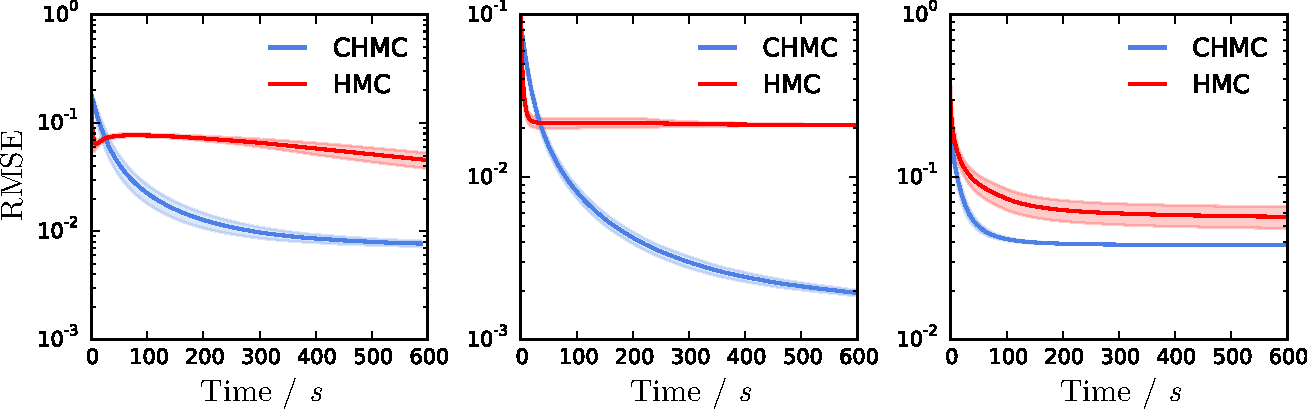
\includegraphics[width=\textwidth]{images/binocular-pose-estimates-rmse.pdf}
  \caption{}
  \label{sfig:pose-binocular-rmses}
\end{subfigure}
\\
\begin{subfigure}[b]{0.7\textwidth}
  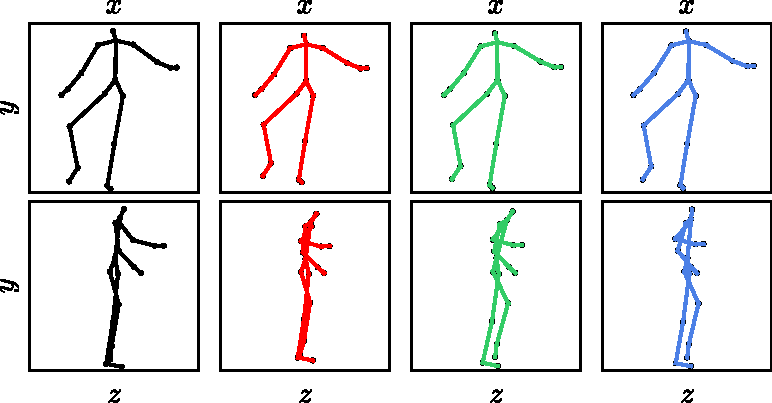
\includegraphics[width=\textwidth]{images/monocular-pose-sample-projections.pdf}
  \caption{}
  \label{sfig:pose-monocular-samples}
\end{subfigure}
\caption[Inference in human pose model.]{\textsf{Human pose}~ (a) \acp{RMSE} of 3D pose posterior mean estimates given binocular projections, using samples from our method (blue) versus running \ac{HMC} in hierarchical model (red) for three different scenes sampled from the prior. Horizontal axes show computation time to produce number of samples in estimate. Solid curves are average \ac{RMSE} over 10 runs with different seeds and shaded regions show $\pm 3$ standard errors of mean. (b) Orthographic projections (top: front view, bottom: side view) of 3D poses consistent with monocular projections. Left most pair (black) shows pose used to generate observations, right three show constrained \ac{HMC} samples.}
\label{fig:pose-inference}
\end{figure}

The experiments in this and the following section have a different emphasis than those in the preceding sections. The models considered here are learnt generative models of complex high-dimensional datasets, in particular human pose and image data. We use these models to perform inference tasks 

For our next experiment we considered inferring a three-dimensional human pose and camera model from two-dimensional projections of joint positions. We used a 19 joint skeleton model, with a learnt prior distribution over poses parametrised by 47 local joint angles $\rvct{z}_a$. The pose model was learnt from the \emph{PosePrior} motion capture data-set \citep{akhter2015pose} with a Gaussian \ac{VAE} \citep{kingma2013auto} trained to match the distribution of the motion capture joint angle data. The circular topology of the angular data is poorly matched by the Euclidean space a Gaussian \ac{VAE} typically learns a distribution on, and simply `unwrapping' the angles to e.g. $[-\pi,\pi)$ leads to unnatural discontinuities at the $\pm \pi$ cut-point, this both making the initial learning problem challenging (as there is no in-built prior knowledge of continuity across the cut-point) and tending to lead to a learned latent space less amenable to \ac{MCMC} inference as `nearby' poses with one or more joint angles on opposite sides of the cut-point will likely end up corresponding to points far apart in the latent space.

During training we therefore mapped each vector of 47 joint angles $\vct{z}_a^{(i)}$ (corresponding to a single motion capture datapoint) to a pair of 47-dimensional vectors $(\vct{r}_1^{(i)},\vct{r}_2^{(i)})$ by sampling a Gaussian random vector $\vct{n}^{(i)} \sim \nrm{\vct{0},\,\idmtx}$ and then computing $\vct{r}_1^{(i)} = \exp\vct{n}^{(i)}\,\odot\,\cos\vct{z}_a^{(i)}$ and $ \vct{r}^{(i)}_2 = \exp\vct{n}^{(i)}\,\odot\,\sin\vct{z}^{(i)}_a$ and training the \ac{VAE} to maximise (a variational lower bound) on the joint marginal density of the $\lbrace \vct{r}^{(i)}_1,\,\vct{r}^{(i)}_2\rbrace_i$ pairs. At the cost of doubling the dimension, this leads to an embedding in a Euclidean space which does not introduce any arbitary cut-points and empirically seemed to lead to better sample quality from the learned generative model compared to learning the angles directly. Given the trained model we can generate a vector of angles $\rvct{z}_a$ using the model by sampling a Gaussian code (latent representation) vector $\rvct{u}_h$ from $\nrm{\vct{0},\idmtx}$ then sampling a pair of 47-dimensional vectors $\rvct{r}_1$ and $\rvct{r}_2$ from the learnt Gaussian decoder model given $\rvct{u}_h$ (and further Gaussian random input vectors $\rvct{u}_1$ and $\rvct{u}_2$), and finally recovering an angle by computing $\rvct{z}_a = \textrm{atan2}(\rvct{r}_2,\rvct{r}_1)$. The resulting distribution on $\rvct{z}_a$ is only implicitly defined, but the overall generative model is differentiable with respect to the input vectors $\rvct{u}_h$, $\rvct{u}_1$ and $\rvct{u}_2$.

The \emph{PosePrior} motion capture data includes recordings from only a relatively small number of distinct actors and so limited variation in the `bone-lengths' of the skeleton model. Therefore a serparate log-normal model for the bone lengths $\rvct{z}_b$ was fitted using data from the \emph{ANSUR} anthropometric data-set \citep{gordon1988ansur}, due to symmetry in the skeleton thirteen independent lengths being specified. A simple pin-hole projective camera model with three position parameters $\rvct{z}_c$ and fixed focal-length was used\footnote{The camera orientation was assumed fixed to avoid replicating the degrees of freedom specified by the angular orientation of the root joint of the skeleton: only the relative camera--skeleton orientation is important.}. A log-normal prior distribution was placed on the depth co-ordinate $\rvar{z}_{c,2}$ to enforce positivity with normal priors on the other two co-ordinates $\rvar{z}_{c,0}$ and $\rvar{z}_{c,1}$. 

Given a generated triplet of joint-angles, bone length and camera parameters $\rvct{z}_a$, $\rvct{z}_b$ and $\rvct{z}_c$, a simulated two-dimensional projection of the skeleton $\rvct{x}$ is produced by first mapping the joint-angles and bone-lengths to a $4 \times 19$ matrix of joint positions $\rvct{P}$ in (homegeneous) world-coordinates by recursing through the skeleton tree. A $3 \times 4$ projective camera matrix $\rvct{C}$ is generated from $\rvct{z}_c$ and then used to project the world-coordinate joint positions to a $2 \times 19$ matrix $\rvct{X}$ of joint positions in two-dimensional image-coordinates. The projected positions matrix $\rvct{X}$ is flattened to a vector and a Gaussian vector with standard deviation $\epsilon$ added to the projected position vector to give the $19 \times 2 = 38$ dimensional observed vector $\rvct{x}$. The noise standard deviation $\epsilon$ is chosen so that the noise in the projected joint positions is non-obvious in generated projections. The overall corresponding model generator functions $\genfunc_{\rvct{x}|\rvct{z}}$ and $\genfunc_{\rvct{z}}$ are described procedurally in Algorithm \ref{alg:pose-model- generators} and a factor graph summarising the relationships between the variables in the model shown in Figure \ref{fig:pose-dgm-factor-graph}.

Although the Gaussian observed output noise is necessarily not needed to apply our proposed constrained \ac{HMC} method as the generator without the final additive noise still defines a valid differentiable generative model, using the noisy observation model means that an explicit hierarchical joint density on is defined on $\fset{\rvct{x},\,\rvct{u}_h,\,\rvct{r}_1,\,\rvct{r}_2,\,\rvct{z}_b,\,\rvct{z}_c}$ allowing comparison of our constrained \ac{HMC} method with (non-constrained) \ac{HMC} as a baseline. Further as discussed previously the adding noise to the output ensures the generator Jacobian is full-rank everywhere and also significantly simplifies the process of finding an initial $\rvct{u}$ such that the generated $\rvct{x}$ matches observations.

We first considered binocular pose estimation, with the variables defining the three-dimensional scene information $\rvct{z}_a$, $\rvct{z}_b$ and $\rvct{z}_c$, inferred given a pair of two-dimensional projections from two simulated cameras with a known offset in their positions (in this case the generator function is adjusted accordingly to output an $19 \times 2 \times 2 = 76$ dimensional observed vector $\rvct{x}$ corresponding to the concatenation of the flattened projected joint positions from both `cameras'). In this binocular case, the disparity in projected joint positions between the two projections gives information about the distances of the correspondings joints from the image plane in the depth direction and so we would expect the posterior distribution on the three-dimensional pose to be tightly distributed around the true values used to generate the observations. We compared our constrained \ac{HMC} method to running standard \ac{HMC} on the conditional density of $\fset{\rvct{u}_h,\,\rvct{r}_1,\,\rvct{r}_2,\,\rvct{z}_b,\,\rvct{z}_c}$ given $\rvct{x}$.

Figure \ref{sfig:pose-binocular-rmses} shows the \ac{RMSE} between the posterior mean estimate of the three-dimensional joint positions and the true positions used to generate the observations as the number of samples included in the estimate increases for three test scenes. For both methods the horizontal axis has been scaled by run time. The constrained \ac{HMC} method (blue curves) tends to give position estimates which converge more quickly to the true position. In this case standard \ac{HMC} performs relatively poorly despite the signficantly cheaper cost of each integrator step compared to the constrained dynamics. This is at leastin part due to the small output noise standard deviation $\epsilon$ used which requires a small integrator step to be used to maintain reasonable accept rates. Relaxing too larger $\epsilon$ values makes the non-constrained approach more competitive but with an associated cost in loss of 

 Visually inspecting the sampled poses and individual run traces (not shown) it seems that the \ac{HMC} runs tended to often get stuck in local modes corresponding to a subset of joints being `incorrectly' positioned while still broadly matching the (noisy) projections. The complex dependencies of the joint positions on the angle parameters mean the dynamic struggles to find an update which brings the `incorrect' joints closer to their true positions without moving other joints out of line. The constrained \ac{HMC} method seemed to be less susceptible to this issue.

We also considered inferring 3D scene information from a single 2D projection. Monocular projection is inherently information destroying with significant uncertainty to the true pose and camera parameters which generated the observations. Figure \ref{sfig:pose-monocular-samples} shows pairs of orthographic projections of 3D poses: the left most column is the pose used to generate the projection conditioned on and the right three columns are poses sampled using constrained \ac{HMC} consistent with the observations. The top row shows front $x$--$y$ views, corresponding to the camera view though with a orthographic rather than perspective projection, the bottom row shows side $z$--$y$ views with the $z$ axis the depth from the camera. The dynamic is able to move between a range of plausible poses consistent with the observations while reflecting the inherent depth ambiguity from the monocular projection.

\subsection{MNIST super-resolution}

\begin{figure}
\centering
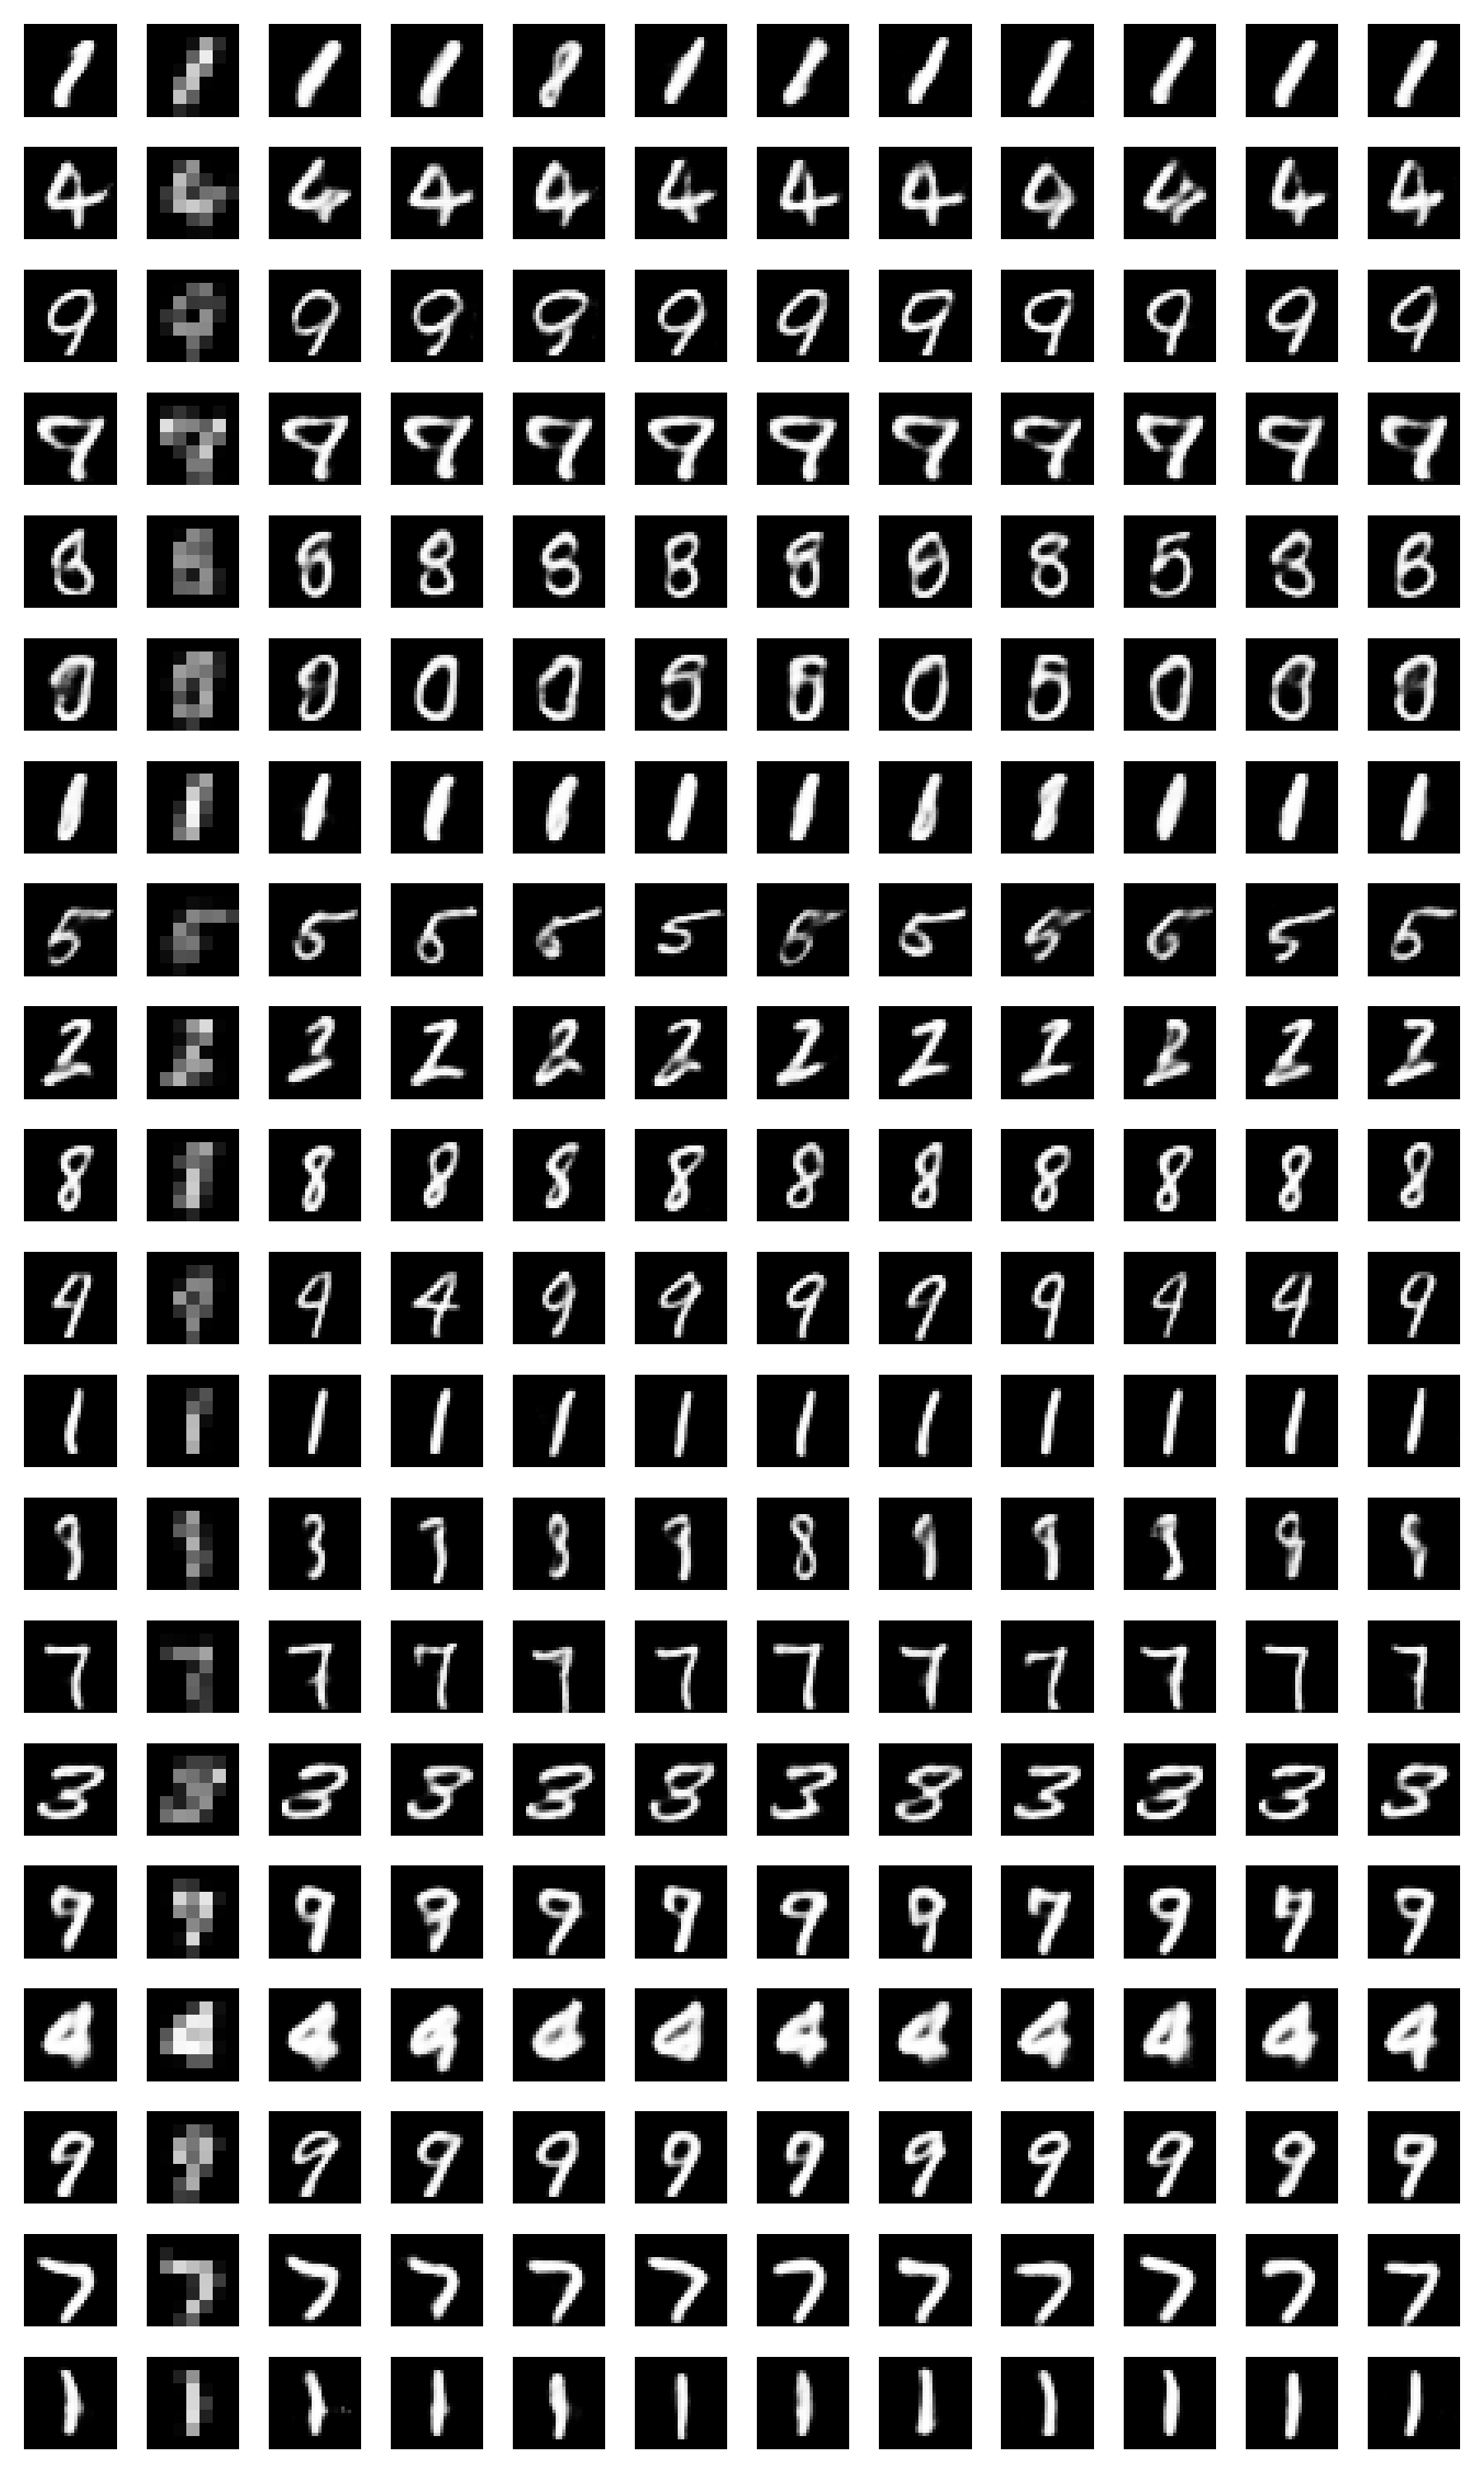
\includegraphics[width=\textwidth]{images/mnist-super-resolution-factor-4.pdf}
\caption[MNIST super-resolution samples.]{MNIST super-resolution samples. In each row the first column shows the original image and the second image the `observed' blurred and downsampled image. The remaining ten columns show sampled full-resolution reconstructions of the image.}
\label{fig:mnist}
\end{figure}

As a final task we considered inferring higher resolution reconstructions of a digit image given a blurred and downsampled observed version. For the generative model, we use a differentiable generator network trained on MNIST digit images combined with a simple observation model consisting of a blurring convolution operation and downsampling step. Though we can easily simulate downsampled images, the density on the generator output is only implicitly defined.


A Gaussian \ac{VAE} trained on MNIST was used as the generative model, with a 50-dimensional hidden code $\rvct{h}$. We compared our method to running \ac{HMC} in the known conditional distribution on $\rvct{h}$ given $\rvct{x}$ ($\rvct{z}$ can then be directly sampled from its Gaussian conditional distribution given $\rvct{h}$).

Example samples are shown in Figure \ref{fig:mnist}. In this case the constrained and standard \ac{HMC} approaches appear to be performing similarly, with both able to find a range of plausible in-paintings given the observed pixels. Without cost adjustment the standard \ac{HMC} samples show greater correlation between subsequent updates, however for a fairer comparison the samples shown were thinned to account for the approximately $40\times$ larger run-time per constrained \ac{HMC} sample. Although the constrained dynamic does not improve efficiency here neither does it seem to hurt it.

\section{Discussion}

The methods discussed in this chapter are intended to help deal with

We have presented a generally applicable framework for performing inference in differentiable generative models. Though simulating the constrained Hamiltonian dynamic is computationally costly, the resulting coherent exploration of the state space can lead to significantly improved sampling efficiency over alternative methods.

The constrained \ac{HMC} approach we propose in some cases allows asymptotically exact inference in differentiable generative models where \ac{ABC} methods might otherwise be used. We suggest an approach for dealing with two of the key issues in \ac{ABC} methods --- enabling inference in continuous spaces as $\epsilon$ collapses to zero and allowing efficient inference when conditioning on high-dimensional observations without the need for dimensionality reduction with summary statistics (and the resulting task of choosing appropriate summary statistics). As well as being of practical importance itself, this approach should be useful in providing `ground truth' inferences in more complex models to assess the affect of the approximations used in \ac{ABC} methods on the quality of the inferences.

In molecular simulations, constrained dynamics are often used to improve efficiency. Intra-molecular motion is removed by fixing bond lengths. This allows a larger time-step to be used due to the removal of high-frequency bond oscillations \citep{leimkuhler2016efficient}. An analogous effect is present when performing inference in an \ac{ABC} setting with a $\epsilon$ kernel `soft-constraint' to enforce consistency between the inputs and observed outputs. As $\epsilon \to 0$ the scales over which the inputs density changes value in directions orthogonal to the constraint manifold and along directions tangential to the manifold increasingly differ. To stay within the soft constraint a very small step-size needs to be used. Using a constrained dynamic decouples the motion on the constraint manifold from the steps to project on to it, allowing more efficient larger steps to be used for moving on the manifold.

A limitation of our method is the requirement of differentiability of the generator. This prevents applying our approach to generative models which use discontinuous operations or discrete random inputs. In some cases conditioned on fixed values of discrete random inputs the generator may still be differentiable and so the proposed method can be used to update the continuous random inputs given values of the discrete inputs. This would need to be alternated with updates to the discrete inputs, which would require devising methods for updating the discrete inputs to the generator while constraining its output to exactly match observations.

As discussed in Section \ref{sec:abc}, a common approach in \ac{ABC} methods is to define the kernel or distance measure in terms of summary statistics of the observed data \citep{prangle2015summary,marin2012approximate}. This is necessary in standard \ac{ABC} approaches to cope with the `curse of dimensionality' with the probability of accepting samples / moves for a fixed tolerance $\epsilon$ exponentially decreasing as the dimensionality of the observations conditioned on increases. Although as already noted the proposed method is better able to cope with high observation dimensions, if appropriate informative statistics are available (e.g. based on expert knowledge) and these are differentiable functions of the generator outputs, they can be easily integrated in to the proposed method by absorbing the statistic computation in to the definition of $\genfunc_{\rvct{x}}$.

\section{Related work}\label{sec:related-work}

%In our setting the gradient of the logarithm of the target density on the manifold \eqref{eq:tgt-density-on-manifold} consists of the sum of $\grad\log\rho$ and $-\frac{1}{2}\nabla\log\left|\jacobian{\genfunc_{\rvct{x}}}\jacobian{\genfunc_{\rvct{x}}}\phantom{}\tr\right|$. The former will typically be cheap compute and as shown in the Appendix the latter can be efficiently computed 

% coupled ABC
% M/G/1 queue Neal
% quantile distributions

\emph{Hamiltonian ABC} \cite{meeds2015hamiltonian}, also proposes applying \ac{HMC} to perform inference in simulator models as considered here. An {ABC} set-up is used with a Gaussian synthetic-likelihood formed by estimating moments from simulated data. Rather than using automatic differentiation to exactly calculate gradients of the generator function, \emph{Hamiltonian ABC} uses a stochastic gradient estimator. This is based on previous work considering methods for using a stochastic gradients within \ac{HMC} \citep{welling2011bayesian,chen2014stochastic}. It has been suggested however that the use of stochastic gradients can destroy the favourable properties of Hamiltonian dynamics which enable coherent exploration of high dimensional state spaces \citep{betancourt2015fundamental}. In \emph{Hamiltonian ABC} it is also observed that representing the generative model as a deterministic function by fixing the random inputs to the generator is a useful method for improving exploration of the state space. This is achieved by including the seed of the pseudo-random number generator in the chain state rather than the set of random inputs.

Also related is \emph{Optimisation Monte Carlo} \citep{meeds2015optimization}. The authors propose using an optimiser to find parameters of a simulator model consistent with observed data (to within some tolerance $\epsilon$) given fixed random inputs sampled independently. The optimisation is not volume-preserving and so the Jacobian of the map is approximated with finite differences to weight the samples. Our method also uses an optimiser to find inputs consistent with the observations, however by using a volume-preserving dynamic we avoid having to re-weight samples which can scale poorly with dimensionality. 

Our method also differs in treating all inputs to a generator equivalently; while the \emph{Optimisation Monte Carlo} authors similarly identify the simulator models as deterministic functions they distinguish between parameters and random inputs, optimising the first and independently sampling the latter. This can lead to random inputs being sampled for which no parameters can be found consistent with the observations (even with a within $\epsilon$ constraint). Although optimisation failure is also potentially an issue for our method, we found this occurred rarely in practice if an appropriate step size is chosen. Our method can also be applied in cases were the number of unobserved variables is greater than the number of observed variables unlike \emph{Optimization Monte Carlo}.
